% -*-latex-*-

%% IMPORTANT: The official thesis specifications are available at:
%%            http://libraries.mit.edu/archives/thesis-specs/
%%
%%            Please verify your thesis' formatting and copyright
%%            assignment before submission.  If you notice any
%%            discrepancies between these templates and the
%%            MIT Libraries' specs, please let us know
%%            by e-mailing thesis@mit.edu

%% The documentclass options along with the pagestyle can be used to generate
%% a technical report, a draft copy, or a regular thesis.  You may need to
%% re-specify the pagestyle after you \include  cover.tex.  For more
%% information, see the first few lines of mitthesis.cls.

%\documentclass[12pt,vi,twoside]{mitthesis}
%%
%%  If you want your thesis copyright to you instead of MIT, use the
%%  ``vi'' option, as above.
%%
%\documentclass[12pt,twoside,leftblank]{mitthesis}
%%
%% If you want blank pages before new chapters to be labelled ``This
%% Page Intentionally Left Blank'', use the ``leftblank'' option, as
%% above.

\documentclass[12pt,oneside]{mitthesis}
\usepackage{feynmp}
\usepackage{caption}
\usepackage{subcaption}
\usepackage{lgrind}
%% These have been added at the request of the MIT Libraries, because
%% some PDF conversions mess up the ligatures.  -LB, 1/22/2014
\usepackage{amsmath}
\usepackage{multirow}
\usepackage{cmap}
\usepackage[T1]{fontenc}
\usepackage{indentfirst}
\usepackage[colorlinks=true,bookmarks=true]{hyperref}
  \usepackage{bookmark}
  \hypersetup{breaklinks=true}

\usepackage{geometry}
\geometry{
    a4paper,
    left=1.5in,
    right=1.0in,
    top=1.0in,
    bottom=1.0in
}

\usepackage{fancyhdr}
\fancypagestyle{plain}{
    \fancyhf{} % clear all header and footer fields
    \fancyhead[R]{\thepage} % page number in top right
    \renewcommand{\headrulewidth}{0pt}
    \renewcommand{\footrulewidth}{0pt}
}

%%todo packages
\usepackage[colorinlistoftodos]{todonotes}

%% Addtional packages
\usepackage{lipsum}

%% This bit allows you to either specify only the files which you wish to
%% process, or `all' to process all files which you \include.
%% Krishna Sethuraman (1990).

%\typein [\files]{Enter file names to process, (chap1,chap2 ...), or `all' to process all files:}
%\def\all{all}
%\ifx\files\all \typeout{Including all files.} \else \typeout{Including only \files.} \includeonly{\files} \fi

\newcommand{\mysignrule}[0]{
    \rule{\linewidth}{0.5pt}\newline
}

%-------------------------------------------
\begin{document}

\hypersetup{pageanchor=false}
\pagenumbering{roman}
\title{Measurement of Neutron Radius of $^{208}$Pb Through Parity Violation in Electron Scattering}

\makeatletter
\author{Siyu Jian} \let\Author\@author
\newcommand{\hometown}{Shandong, China}

\prevdegrees{M.S., China Institute of Atomic Energy, China, 2012}
\prevdegrees{B.S., Shandong University, China, 2012}

\department{Department of Physics}
\degree{Doctor of Philosophy}
\degreemonth{Apr}
\degreeyear{2023} \let\Year\@degreeyear
\thesisdate{Apr 30, 2023}
\makeatother

\supervisor{Nilanga Liyanage}{Professor}
\chairman{Kent Paschke}{Professor}

\makeatletter
\def\maketitle{\begin{titlepage}
\doublespacing
\vspace{0.0in}
\large
{\LARGE\bf \@title \par}
\@author \\
\hometown
\par
\@prevdegrees
\par
A Dissertation Presented to the Graduate Faculty \\
of the University of Virginia in Candidacy for the Degree of \\
\@degree
\par
\@department \\
University of Virginia \\
\@degreemonth, \@degreeyear \\
\vspace{1.0in}

\begin{flushright}
\begin{minipage}{0.45\linewidth}
\mysignrule{}
\mysignrule{}
\mysignrule{}
\mysignrule{}
\end{minipage}
\end{flushright}

\end{titlepage}}
\makeatother
\maketitle

% Copyright page
\pagenumbering{roman}
\pagestyle{plain}
\newpage
\vspace*{\fill}
\noindent \textcopyright Copyright by \Author {} \Year \\
All Rights Reserved

\cleardoublepage

% Abstract page
\vspace{0.8in}
\pdfbookmark[0]{Abstract}{Abstract}
\section*{\center Abstract}
\input{abstract}

\cleardoublepage

% Acknowledgemnt page
\pdfbookmark[0]{Acknowledgments}{Acknowledgments}
\section*{Acknowledgments}
This is the acknowledgement section.

Para. 1

adv
\begin{itemize}
    \item GEM 
    \item tremendous help
    \item flexibility of the course
    \item importance of the course in my career
\end{itemize}


Para. 2 
clg
\begin{itemize}
    \item 
\end{itemize}

Para. 3
\begin{itemize}
    \item 
\end{itemize}

\hypersetup{pageanchor=true}

\hypersetup{linkcolor=black}
\pagestyle{plain}
\include{contents}
\hypersetup{linkcolor=red}

\pagenumbering{arabic}
\chapter{Introduction (10)}

In 1961, Robert Hofstadter wins Nobel Price for his pioneering studies of the structure of nucleons with electron scattering. Accelerated electron beams have been widely used to study the inner structure of the nucleons (and neutrons) since then. That experiment can provide different level structure information of nucleons given different incident electron energy. At the range where the energy of electrons is deficient, $\lambda \gg r_p$, here $r_p$ is the proton's radius, $\lambda$ is the electron wavelength, the scattering is equivalent to scattered over point like spin-less object. At a low electron energy range where $\lambda ~r_p$, the scattering is equivalent to scattering over the charged object. When the electron wavelength $\lambda < r_p$, the electron scattering will be able to see the substructures. At a very high energy range where $\lambda \ll r_p$, the electrons are equivalent to scattering over the sea of quarks and gluons of the protons. 

Para. nucleus structure

Para. 
\begin{itemize}
    \item Hofstadter initiates work
    \item our current understanding of the nucleus structure
\end{itemize}

Para.

\begin{itemize}
\item history of the nuclear structure
    \item nucleus structure, how to understand it
    \item charge radius measurement [merge with chapter 2?]
    \item scatter is used for nuclear structure probe, charge radius 
\end{itemize}


Para. 

\begin{itemize}
    \item EM force, nuclear force
    \item neutron density and assumptions
\end{itemize}


\begin{itemize}
    \item neutron charges 0, poorly measured
    \item historical measurement 
    \item parity violation measurement of the neutron density
\end{itemize} 

\section{Rich Physics Behind the PRex Experiment}
\subsection{Neutron density of neutron-rich matter}
\subsection{neutron density theory and corrections to APV}
\subsection{neutron radius measurements}
\subsection{Gravity waves, EOS, and neutron stars}
\subsection{Atomic Parity Non-Conservation Experiment}

\section{Previous Experiment}
\subsection{current theory of the neutron density}

\section{Historical measurement[to be added, move to chapter 1]}
\subsection{Pb charged radius measurement and its result }

\section{Impact of the experiment, result based on PRex-II experiment [move to chapter 6 conclusion]}

\subsection{calculate with Coulomb energy differences Phys. Lett 29B 396 (1969)}
\subsection{L. Ray and G.W.Hoffmann Physics Rev C 31. 538 (1985)}
\subsection{ Parity Violating Measurements of the Neutron Density, C.J. Horowitz, etc}
\subsection{PRex-I experiment}
\chapter{The Theory of PRex Experiment(~20)}
% \todo[inline]{Separate the theory and the experiment part into two chapters}
\begin{itemize}
    \item history of the nuclear structure
    \item scatter is used for nuclear structure probe, charge radius 
    \item neutron charges 0, poorly measured
    \item historical measurement 
    \item parity violation measurement of the neutron density
\end{itemize}

The RMS radius of the  neutron distribution in a heavy nucleus  $R_N$ provides an important test of nuclear theory. Furthermore,   $R_N$ is used in the determination of  the density dependence of symmetry energy of neutron-rich matter; this dependence is an  important input in   neutron star structure, heavy iron collision and atomic parity violation experiment calculations. In the past hadron scattering experiments with pion, proton or anti-proton beams have been used to determine the neutron radii of heavy nuclei. However, these measurements suffer from uncertainties associated with the probe particle and the target nucleus. Electron scattering provides a model-independent probe of nuclear radii.  However, in electron scattering, the measurement of neutron distribution in a nucleus  is much harder than the measurement of the proton distribution  since the neutron is uncharged. 
\section{current theory and limitations}
\section{theory aspect}
\subsection{apv}
\section{Electromagnetic scattering via $\gamma$ exchange}
\section{Proton density}
\subsection{form factor}
\subsection{EM interaction with the exchange of photon}
\subsection{weak interaction with exchange of $Z^0$ Boson}
\section{Parity Violation}
\section{Parity Violation Asymmetry}
\section{Measure neutron density with Parity Violating electron scattering}


% \section{electron scattering}

% In 1961, Robert Hofstadter wins Nobel Price for his pioneering studies of the structure of nucleons with  electron scattering. Accelerated electron beams are widely used for study the inner structure of the nucleons (and neutrons) since then. That experiment can provide different level structure information of nucleons given different incident electron energy. At the range where the energy of electrons are very low, $\lambda \gg r_p$, here $r_p$ is the radius of the proton, $\lambda$ is the electron wavelength, the scattering is equivalent to scattered over point like spin-less object. At low electron energy range where $\lambda ~r_p$, the scattering is equivalent to scattering over charged object. When the electron wavelength $\lambda < r_p$, the electron scattering will be able to see the substructures. At very high energy range where $\lambda \ll r_p$, the electrons is equivalent to scattering over the sea of quarks and gluons of the protons. 

% In one photon exchange approximation, the  transition current for nucleon can be write as:

% $$
% J^\mu = e\bar{\mu}\Gamma^\mu(p)e^{i\vec{q}\vec{x}}$$
% $$

% \todo[inline]{Add the Feynman diagram}

% In one photon exchange approximation, the cross section of electron scattered over spin-0 particle would be:

% $$
% \frac{d\sigma}{d\Omega} = \frac{d\sigma}{d\Omega}|F(Q^2)|
% $$

% \todo[inline]{current result of proton radius (PRad)}

% \subsection{e-p scattering with exchange of photon}
% \subsection{weak interation with exchange of $Z^0$ Boson}
% \subsection{form factor}


% \section{Parity Violation}
% \section{Parity Violation Asymmetry}
% \section{Rich Physics Behind the PRex Experiment}
% \subsection{EOS of Neutron rich matter}
\chapter{Experiment Setup ~20}

\section{Jefferson Lab CEBAF}

The PRex and CREx experiments are conducted at the Continuous Electron Beam Accelerator Facility (CEBAF) housed within Jefferson Lab. Since its inception in the early 1990s, CEBAF has been a global pioneer, forging paths in nuclear physics research.

The heart of CEBAF is its linear accelerators (linacs), specifically the North and South linacs. These linacs serve as the key elements where electrons amass energy, essential for the facility's experimental proceedings. Connecting these two linacs are the Recirculation Arcs, which are magnetic systems designed to curve the electron beam, redirecting it back into the linacs for additional energy enhancement during successive passes. An added function of the Recirculation Arcs is to facilitate the separation of electron beams of varying energy levels, post their multiple circulations through the linacs. This structural alignment and the operational interplay between the components ensure precision and efficacy in executing complex nuclear physics experiments like PRex and CRex.


% Para. 2
% \begin{itemize}
%     \item 12GeV upgrade
%     \item RF separator
%     \item RF cavities, cooled 
%     \item Beam energy and current ability
%     \item accelerated up to 5 times though both linacs, producing a nominal energy of 10.9GeV. 
%     \item 1497MhZ split into three 499MHz.
%     \item north and south linacs each can gen 1.1GeV 
%     \item East/West Arc bend the beam to accelerate again 
%     \item Hall ABC, 10.9GeV 
%     \item Hall D 12GeV
% \end{itemize}

The Jefferson Lab's CEBAF upgrade project, completed in 2014, introduced a number of significant enhancements. The modifications included the addition of five cryomodules to each Linac section, each housing 7-cell cavities capable of handling a higher RF field, courtesy of advanced surface treatments.

Each of these upgraded linacs can now facilitate an energy gain of 1.1 GeV, enabling the electron beam to achieve 2.2 GeV during each circulation. Post traversing the south linac, the electron beam can be partitioned into three distinct 499 MHz beams.

The facility's design allows for the electron beam to be accelerated up to five times through both linacs, producing a nominal energy output of 10.9 GeV. Experimental Halls A, B, and C each can receive a beam carrying energy that is one-fifth of the full 5-pass energy. Additionally, the beam directed to Hall D can be re-accelerated in the north linac, reaching energy levels as high as 12 GeV. This upgrade has elevated the capacity and flexibility of the CEBAF, further enhancing its research potential.

% Para. 3
% \begin{itemize}
%     \item PRex requires high polarized beam 
%     \item high current to be able to get enough statistics to be able to measure 
%     \item PRex experiment choose CEBAF
%     \item high current
%     \item polarize beam ability
% \end{itemize}

The PRex-II and CREx experiments aim to quantify the thickness of the neutron skin by analyzing parity-violated asymmetry. To achieve a reliable measurement with a sufficient confidence interval, a significant volume of statistical data is required. This necessity is met by the capabilities of CEBAF, which can generate a polarized electron beam with a current reaching up to $200 uA$ and a polarization level in the range of $80-90\%$. Such robust performance plays a pivotal role in enabling the execution and success of the PRex and CREx experiments.


\begin{figure}
     \centering
     \begin{subfigure}[b]{0.45\textwidth}
         \centering
         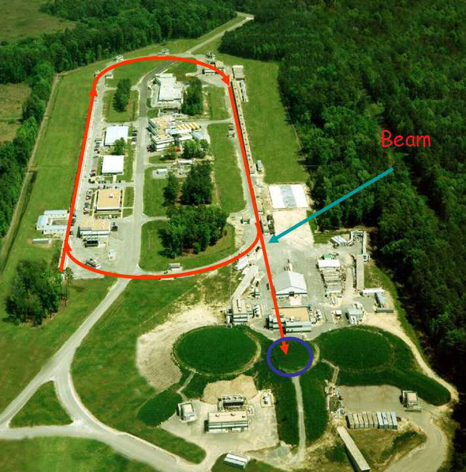
\includegraphics[width=\textwidth]{images/chap3/JLab_cebaf_photo.png}
         \caption{Photo of CEBAF}
         \label{Photo of CEBAF}
     \end{subfigure}
     \hfill
     \begin{subfigure}[b]{0.45\textwidth}
         \centering
         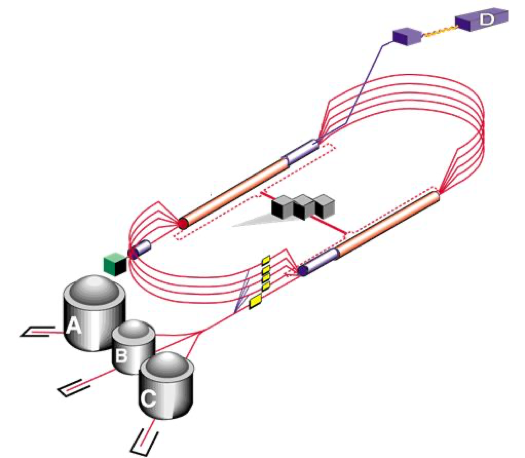
\includegraphics[width=\textwidth]{images/chap3/JLab_cebaf.png}
         \caption{JLAB CEBAF}
         \label{JLAB CEBAF}
     \end{subfigure}
\end{figure}

\section{Beam injection}
% Para. 1 & 2
% \begin{itemize}
%     \item key componet to generate polarized beam
%     \item GaAs photocathode
%     \item three different structure $30-40\%$, $50\%$, $100\%$ which is using now. Engy band plot
%     \item plot/structure of the GaAs photocathode
% \end{itemize}

The polarized electron source at Jefferson Lab comprises a specialized polarized laser system and gallium arsenide (GaAs) photocathodes. This integral apparatus permits the generation of a polarized, or spin-aligned, electron beam. This feature is indispensable for a broad range of experiments conducted at our facility, particularly those probing spin-dependent phenomena.

The GaAs photocathode is irradiated with circularly polarized laser light possessing energy exceeding the bandgap energy. This triggers the emission of electrons that exhibit specific spin polarization, a process attributable to the photoelectric effect.

\begin{figure}[!htbp]
    \centering
    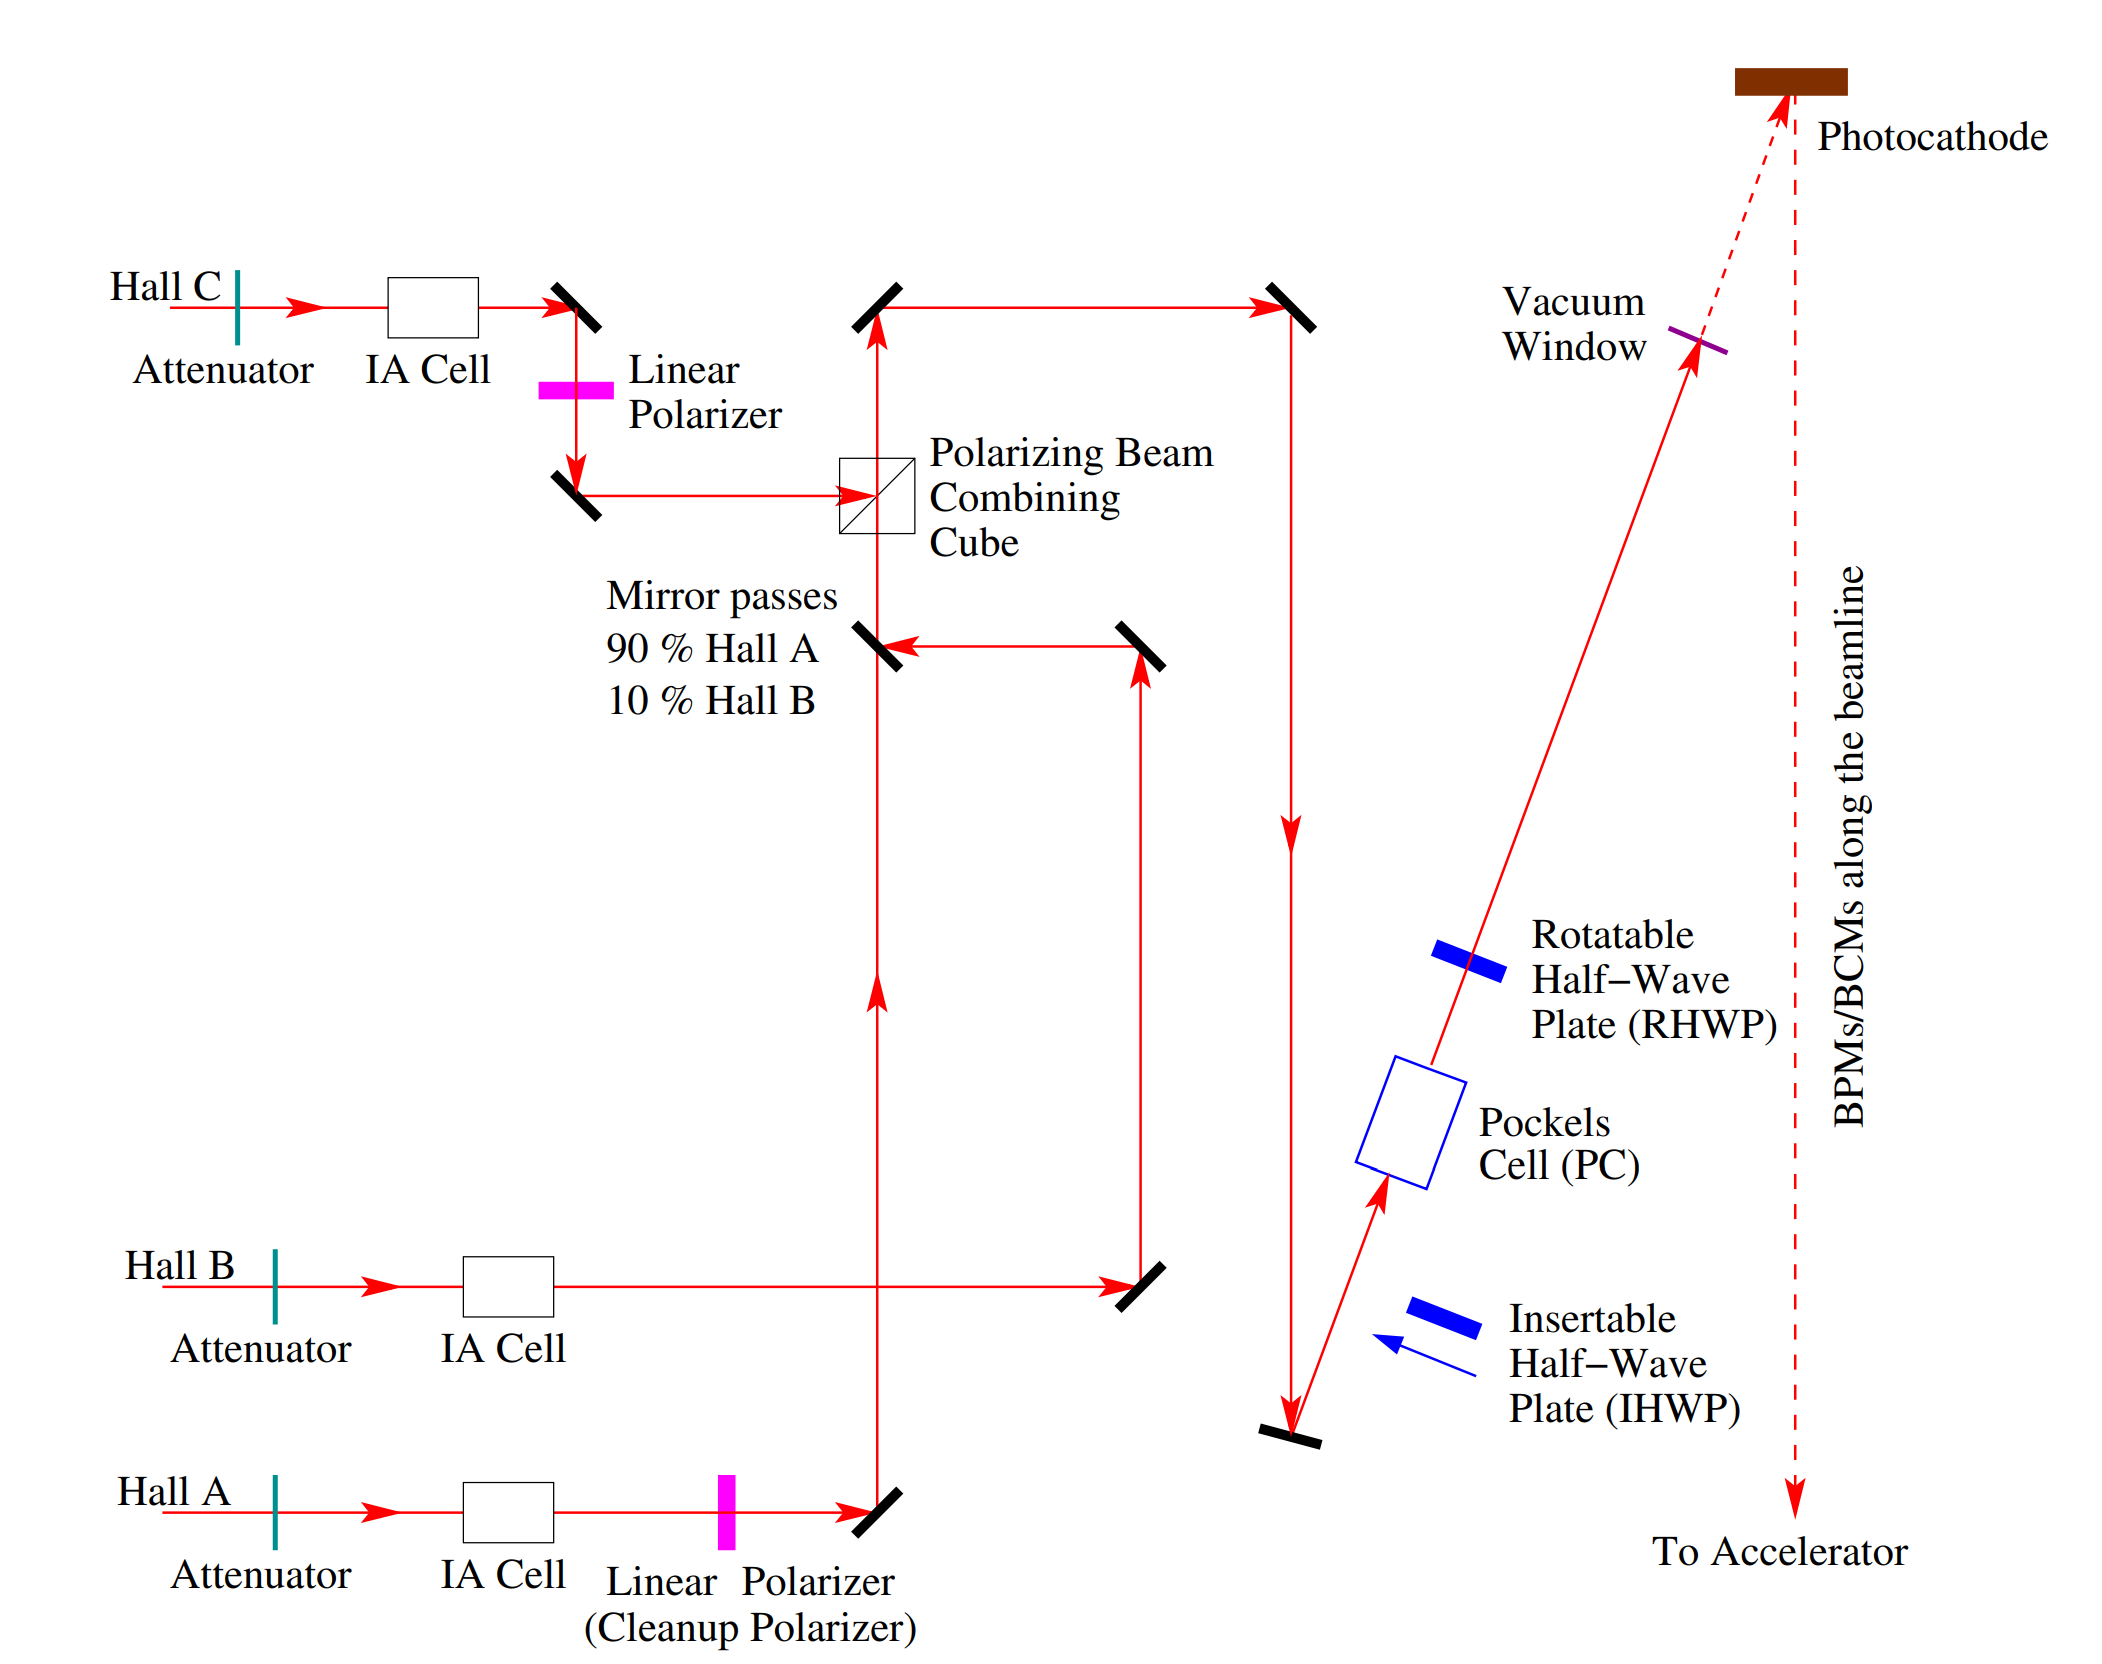
\includegraphics[width=\textwidth]{images/chap3/jlab_polarized_source.png}
    \caption{Schema of the Polarized Laser system in the injector. add REF}
    \label{fig:cebaf_polarize_laser_system}
\end{figure}
\subsection{Polarized Beam Source}

The polarization of the electron beam is quantified by the following equation:

\begin{equation}
p = \frac{N{\uparrow} - N{\downarrow}}{N{\uparrow} + N{\downarrow}}
\end{equation}

Here, $N$ represents the number of electrons in the conduction band of each corresponding spin state. 

The generation of polarized electrons in our source is underpinned by the photoemission process from negative-electron-affinity III-V semiconductor materials, notably Gallium Arsenide (GaAs). The electron spin polarization observed arises from the unique crystal symmetry of GaAs, which governs transitions from the fully occupied valence band to the normally vacant conduction band, akin to transitions from a state with total angular momentum j=3/2 to one with j=1/2. For bulk GaAs as showed in the plot [todo ADD THE energy plot], permits two transitions between the valence band and the conduction band. For every given excitation, three times as many electron spins are anti-parallel to the photon spin than parallel to it. as a result, in theory the maximum polarization can achieve is $50\%$. But in practice, the polarization is around $30-40\%$. 


Addressing this limitation, T. Maruyama and colleagues at the Stanford Linear Accelerator (SLAC) pioneered the use of strained GaAs to increase the polarization rate, \cite{PhysRevLett.66.2376}. This approach achieved an enhanced polarization rate of approximately $70\%$. The technique of strained GaAs involves the epitaxial growth of an InGaAs surface layer on GaAs. The resulting crystal-lattice mismatch between these two compounds introduces an axial strain. This strain effectively breaks the degeneracy of the $P_{3/2}$ valence band energy levels, thereby providing a mechanism to restrict optical excitation from the undesired valence-band spin state. This advancement represents a significant stride in the optimization of electron beam polarization. However, strained GaAs has its own challenges, notably a lower quantum efficiency (QE), which is typically on the order of $0.1\%$. Efforts to augment the QE, for instance, by increasing the thickness of the strained layer, tend to result in a concomitant decrease in polarization, presenting a trade-off that must be carefully managed in practical applications.

The modern photocathodes employ a superlattice structure, composed of numerous thin-layer pairs of lattice-mismatched materials. This design amalgamates the advantages of numerous thin strained layers to simultaneously achieve high polarization and high QE. The photocathode uses in Jefferson Lab achieves approximately $90\%$ polarization while maintaining a quantum efficiency of about $1\%$. \cite{PhysRevB.13.5484}, \cite{ADDERLEY2023167710}


[bulk GaAs figure]

[strain GaAs figure]

[super-lattice GaAs figure]

[add energy level figure]

\subsection{Helicity Control}
Helicity plays a pivotal role in the PRex/CRex experiments. For the minimization of systematic errors, it is imperative to quickly and consistently flip the helicity, or spin direction, of the electron beam. The Pockels Cell (PC) is instrumental in facilitating this helicity reversal. This device is indeed crucial for the PRex experiment as it enables rapid, precise control over the electron beam's helicity, a vital requirement for measuring neutron distribution.

The heart of the Pockels cell consists of two piezoelectric crystals made of Rubidium Titanyl Phosphate. When voltage is applied to these crystals, they can transform linearly polarized laser light into either left or right circularly polarized light. This polarization alteration directly affects the helicity of the electron beam. By modulating the voltage applied to the crystals, the beam's helicity can be swiftly adjusted. For the PRex-II experiment, the helicity flip rate was set at 240Hz.[REF pockels cell board paper] 

\section{Beam monitor}

Numerous beam monitors operate within CEBAF (Continuous Electron Beam Accelerator Facility) to ensure its functionality aligns with the experimental requirements. Among these monitors, the polarimeter, beam position monitor, and beam current monitor play significant roles in the success of the PRex/CRex experiments. This section provides a concise introduction to these vital monitoring systems, offering an insight into their operations and their importance in maintaining the integrity of the experiment.

\subsection{polarimeters}

\subsubsection{Mott Polarimeter}



\subsubsection{Compton Polarimeter}

The Compton polarimeter in Jefferson Lab's Continuous Electron Beam Accelerator Facility (CEBAF) Hall A is another essential instrument used to measure the polarization of the electron beam. Unlike the Møller polarimeter, which relies on electron-electron interactions, the Compton polarimeter operates based on the principle of Compton scattering.

Compton scattering involves the interaction between a beam of electrons and a photon, typically originating from a laser. The electrons scatter off the photons and experience a change in energy and direction depending on the incident photon's energy and the scattering angle. The change in energy of the scattered electrons (or alternatively, the scattered photons) is directly related to the polarization of the incident electron beam.


In the Compton polarimeter in Hall A, the beam is directed into the optical cavity by two dipole magnets. A high-powered, circularly polarized laser is strategically positioned inside the cavity to intersect the electron beam. This encounter leads to Compton scattering, thereby generating scattered photons and electrons. However, only a minute fraction of the electron beam interacts with the polarized photons. Post-scattering, the beam is deflected back to the beam line. The scattered electrons are detected using electron detectors, which comprise plates of synthetic diamonds developed through chemical vapor deposition. Compton-scattered photons are identified within an array of lead tungstate (PbWO4) crystals.

A unique advantage of the Compton polarimeter is its capacity to assess the beam's polarization without disrupting its operation. This feature facilitates uninterrupted, real-time monitoring of the beam's polarization during experiments. The disparity in count rates between the two helicity states serves as an indicator of the beam's polarization, thereby enhancing the accuracy and reliability of the measurements.


\begin{figure}[!htbp]
    \centering
    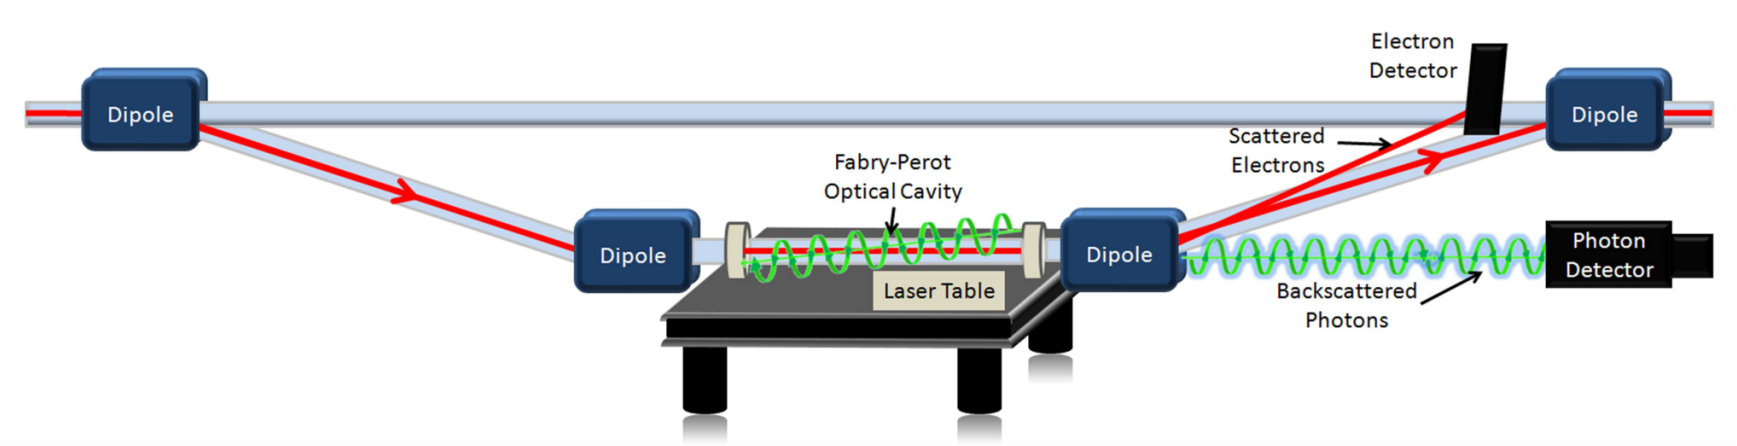
\includegraphics[width=\textwidth]{images/chap3/compton.png}
    \caption{Caption}
    \label{fig:enter-label}
\end{figure}


% \begin{equation}
%     A_{exp} = \frac{n^+-n^-}{n^++n^-} = P_{\gamma}P_e<A_{th}>
% \end{equation}

\subsubsection{Moller Polarimeter}

The Møller polarimeter operates by detecting the electrons scattered from a polarized target, leveraging the phenomenon known as Møller scattering. This type of electron-electron scattering happens when two electrons interact, and the outcome of this interaction is measured. Significantly, the probability of scattering is deeply influenced by the relative spin orientations of the interacting electrons. This property makes Møller scattering particularly beneficial for gauging beam polarization. Unlike the Compton polarimeter, however, the Møller polarimeter cannot operate simultaneously with the production run.

In the ultra-relativistic limit, the Møller asymmetry can be expressed as:

\begin{equation}
A_{exp} = P_{beam}P_{targ}<A_{zz}>
\end{equation}

In this equation, $<A_{zz}>$ represents the average analysis power over the captured cross-section, given by:

\begin{equation}
A_{zz} = \frac{\sin^2{\theta(7 + \cos^2{\theta})}}{(3 + \cos^2{\theta})^2}
\end{equation}

\begin{figure}[!htbp]
    \centering
    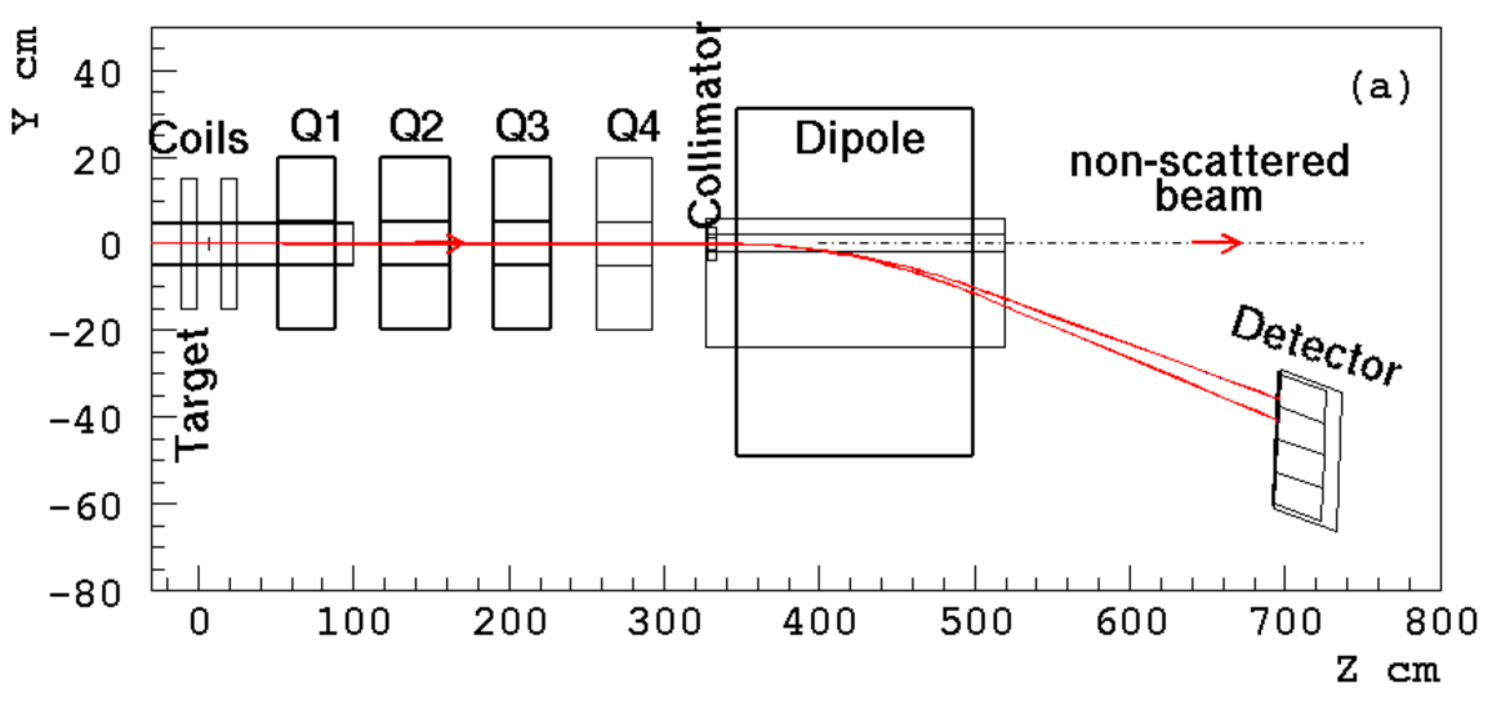
\includegraphics[width=\textwidth]{images/chap3/moller.png}
    \caption{moller, need to re-plot}
    \label{fig:enter-label}
\end{figure}

\subsection{Beam Position Monitor}

The beam position is a critical parameter for calculating the kinematics of electron scattering. Various Beam Position Monitors (BPMs) are installed throughout CEBAF to ensure the beam operates optimally. In the PRex-II/CRex experiment, two types of BPMs are mainly employed: one suited for high current beam position measurements, and a low current cavity monitor used when the beam current is low.

Each BPM features a four-wire antenna, placed diagonally along the beamline and denoted as $V_+$, $V_-$, $U_+$, and $U_-$. As the beam traverses the BPM, it induces a current in the antenna, the amplitude of which is proportional to the beam's position and intensity. Figure \ref{fig:cebaf_beam_position_monitor} illustrates the BPM's structure.

The position of the beam along the BPM's antenna-rotated coordinate system can be expressed as:

\begin{equation}
x' = c_x\frac{V_+ - V_-}{V_+ + V_-}
\end{equation}
\begin{equation}
y' = c_y\frac{U_+ - U_-}{U_+ + U_-}
\end{equation}

In these equations, $c_x$ and $c_y$ denote calibration constants. The hall coordinate system is rotated from the BPM's wire direction by $45^\circ$. With the rotation matrix, the position measured by the BPM in the hall coordinate system can be represented as:

\begin{equation}
x_{bpm} = x'\cos{\theta} - y'\sin{\theta}
\end{equation}
\begin{equation}
y_{bpm} = x'\sin{\theta} + y'\cos{\theta}
\end{equation}

Here, the rotation angle $\theta = 45^\circ$. Beam Position Monitor A (IPM1H03A, BPMA) is situated $7.524m$ upstream of the target, and Beam Position Monitor B(IPM1H03B, BPMB) is $1.286m$ upstream of the target.



\begin{itemize}
    \item cavity for low current measurement 
    \item harp for bpm collaboration
\end{itemize}

\subsection{Beam current monitor}

In the PRex-II and CRex experiments conducted at Jefferson Lab, the Beam Current Monitor (BCM) is used for the precise measurements of beam current and beam charge. Engineered for stability, minimal noise, and non-intrusive operation, the BCM is strategically situated about 25 meters upstream of the target.

At its core, the BCM features a Parametric Current Transformer (PCT) sensor, commonly known as an Unser monitor, and a pair of RF cavity monitors. The PCT toroid is designed to be responsive to the direct current (DC) component of the magnetic field, generated by the beam current as it encircles the beam pipe.

To mitigate the impact of parasitic currents, a ceramic gap interrupts the conductivity of the beam pipe within the toroid. Moreover, the system employs three magnetic shields—two comprised of iron and the innermost one of µ metal—to counteract offset drifts induced by fluctuating external magnetic fields.

The entire assembly is encased in a thermoregulated enclosure that further curtails PCT offset drifts. An electrical shield is implemented to prevent high frequencies in the beam spectrum from escaping the monitor via the ceramic gap. Additionally, materials with high absorption capacity are used to shield the sensor from RF noise, ensuring that the BCM consistently delivers accurate and reliable measurements.

\begin{figure}[!htbp]
    \centering
    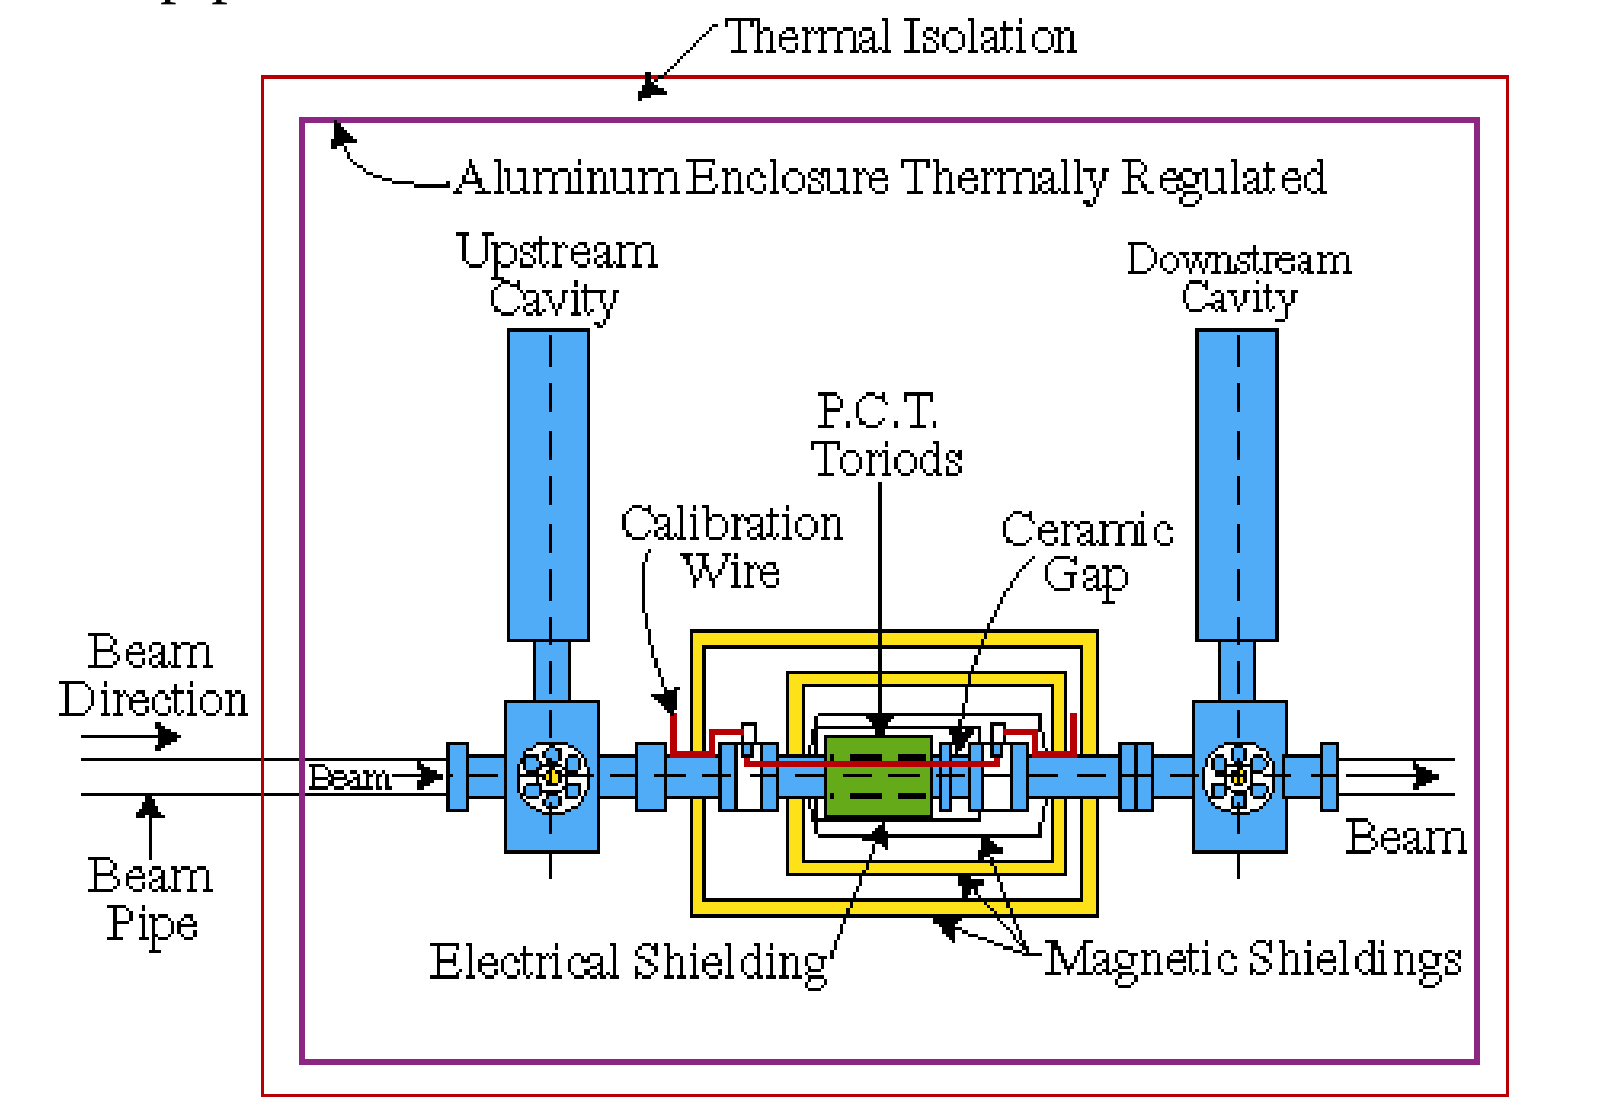
\includegraphics[width=\textwidth]{images/chap3/beam_current_monitor.png}
    \caption{Caption (SOURCE)}
    \label{fig:enter-label}
\end{figure}


\subsection{Raster}

Generally speaking, the beam size in Jefferson Lab's CEBAF is typically on the order of hundreds of micrometers (${\mu}m$) in diameter. This is a quite small size, which is why the beam can deposit a large amount of energy in a small area and why rastering is necessary when delicate or thin targets are used in experiments to avoid damage to the target.

In Hall A, the raster system includes two sets of air-core dipoles positioned upstream of the Compton polarimeter. Each set of dipoles is driven by an independent power supply, which allows for independent control of the horizontal and vertical dimensions of the rastered beam spot. In the PRex experiment, the rastered beam sport are set to $2cm \times 2 cm$ or $4cm \times 4cm$.

[....... to be added]

Para. to be added
\begin{itemize}
    \item spot++ [used to get the beam plot]
    \item rostered beam plot [find the slides]
    \item calibration of the raster on the beam position which will affect the momentum calibration HRS calibration [slides]
\end{itemize}

\subsection{Beam energy monitor, Tiefenhach measurement}

[..... to be added]

\section{Target System}

The experiments conducted in Jefferson Lab employ two separate target ladders, each hosting different types of targets for specific purposes. The production ladder is equipped with the main targets used for the experiments, while the optics ladder carries calibration targets.

Each target ladder is independently affixed to a motion system and can be controlled separately from the counting-house. As required, these targets can be positioned accurately along the central beamline during the experiment.

\begin{figure}[!htbp]
    \centering
    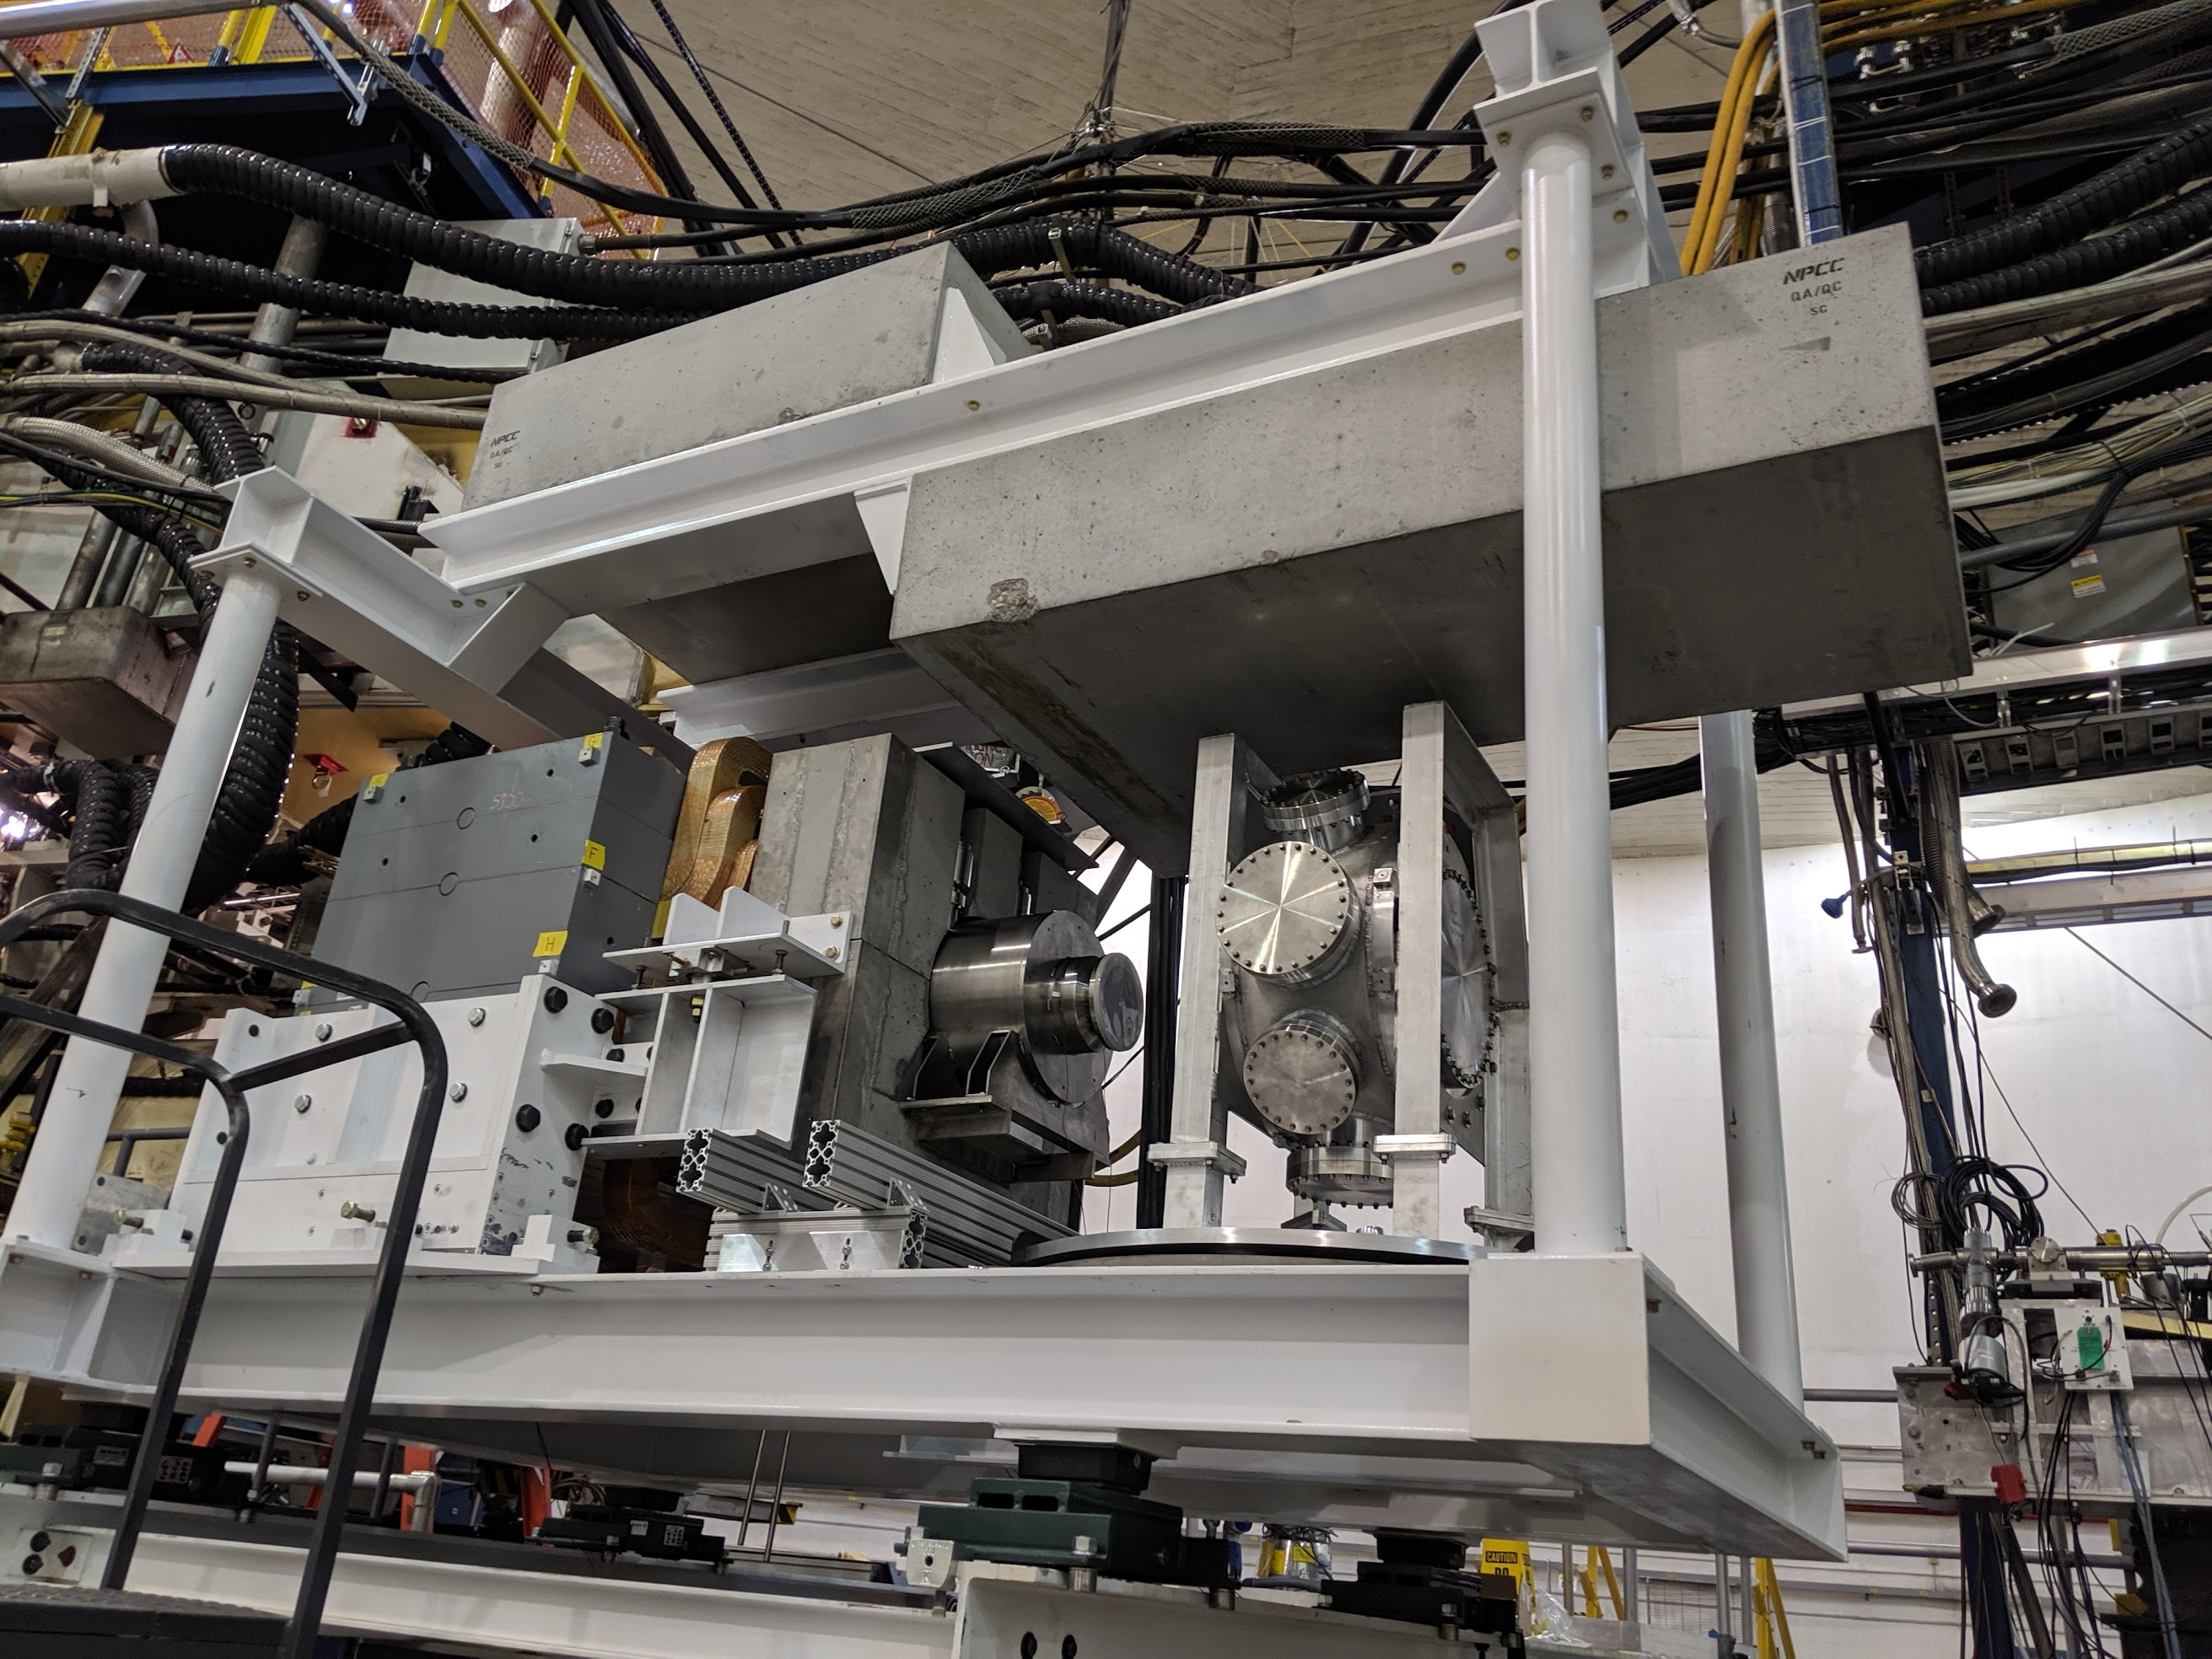
\includegraphics[width=\textwidth]{images/chap3/target_chamber.jpg}
    \caption{Target Chamber used in PRex-II/CRex experiment}
    \label{fig:target_chamber_photo}
\end{figure}

The production target ladder comprises ten 208Pb-D targets, a Carbon target at $1\%$ density, a Carbon hole target designed for alignment purposes, and a Ca48 target. To maintain their performance under high-intensity beam conditions, the targets on the production ladder are cooled with liquid helium at 15K. Of particular note for the PRex experiment are the 208Pb targets. These targets are approximately 0.5mm thick and sandwiched with diamond foils to enhance thermal conductivity, thereby helping to dissipate the power deposited by the beam.

The optics ladder, on the other hand, houses five targets used for High-Resolution Spectrometer (HRS) optics calibrations. These targets, cooled by water, include a natural Pb target, tungsten target, carbon foil target, carbon hole target, and a falling water target developed by INFN. Among them, the Carbon foil is employed for HRS optics calibration and the water target is for pointing measurements. These measurements enable the accurate determination of the HRS angles. The detailed procedures related to these calibration processes will be thoroughly discussed in Chapter 5.

[... more]

\begin{itemize}
    \item Ca target
    \item carbon hole 
\end{itemize}


\section{High Resolution Spectrometer}

The High-Resolution Spectrometers (HRSs) in Hall A of Jefferson Lab are integral components designed specifically for precision measurements of scattering processes. Capable of high-precision particle detection, these instruments allow scientists to delve into the exploration of subatomic matter structures.

Hall A is equipped with two such HRSs, each capable of measuring momentum with an exceptional resolution of up to $0.01\%$. These spectrometers maintain a broad horizontal angular acceptance of ±28 milliradians (mr) and a vertical acceptance of ±60 mr. Strategically positioned on either side of the beamline, each spectrometer can rotate within a plane perpendicular to the beamline, accommodating angles between 12.5 to 150 degrees. This extensive angular range permits the spectrometers to capture scattered particles across a diverse spectrum of kinematic conditions.

In the context of the PRex and CRex experiments, both spectrometers are adjusted to detect scattered electrons at an angle of 5 degrees to maximizes the number of events collected during the experiment. To complement the minimum acceptance angle of the HRSs, an additional spectrometer magnet is incorporated to pre-bend the particles prior to their entry into the HRS.

Positioned within a shield house, the detector package is composed of a range of detectors, each designed for a specific role in measuring the attributes of scattered particles. The detectors are equipped to assess position, angle, and timing of incoming particles. This trio of information is pivotal in determining their momentum and classification, thus forming a comprehensive overview of the particle's properties.

[.... to be added, the HRS plot]

\subsection{collimeter}
[... merge with the sieve slit collimator]

The collimator, a crucial component in the PREx-II and CREx experiments, is strategically positioned between the target chamber and the septum magnet. It is designed with three holes: the central hole permits the unscattered beam to proceed toward the beam dump, while the two uniquely curved holes on the left and right guide and shape the spectrometer's acceptance.

The design of these spectrometer holes is meticulously optimized to enhance the High-Resolution Spectrometer's (HRS) acceptance for the figure of merit. Another significant part of the collimator is the Sieve slit, as depicted in the plot, which plays a critical role in calibrating the optics.

The collimator features a remote actuation capability, which allows for positioning the Sieve optics collimator between the 'beam out' and 'beam in' positions as required. This design allows for precise adjustments in real time during experiments, providing great control and flexibility in achieving optimal results.

[... add the detailed structure of the collimator]

[figure .... collimator in the beamline]

[figure .... sieve in the beamline]


\begin{figure}
     \centering
     \begin{subfigure}[b]{0.45\textwidth}
         \centering
         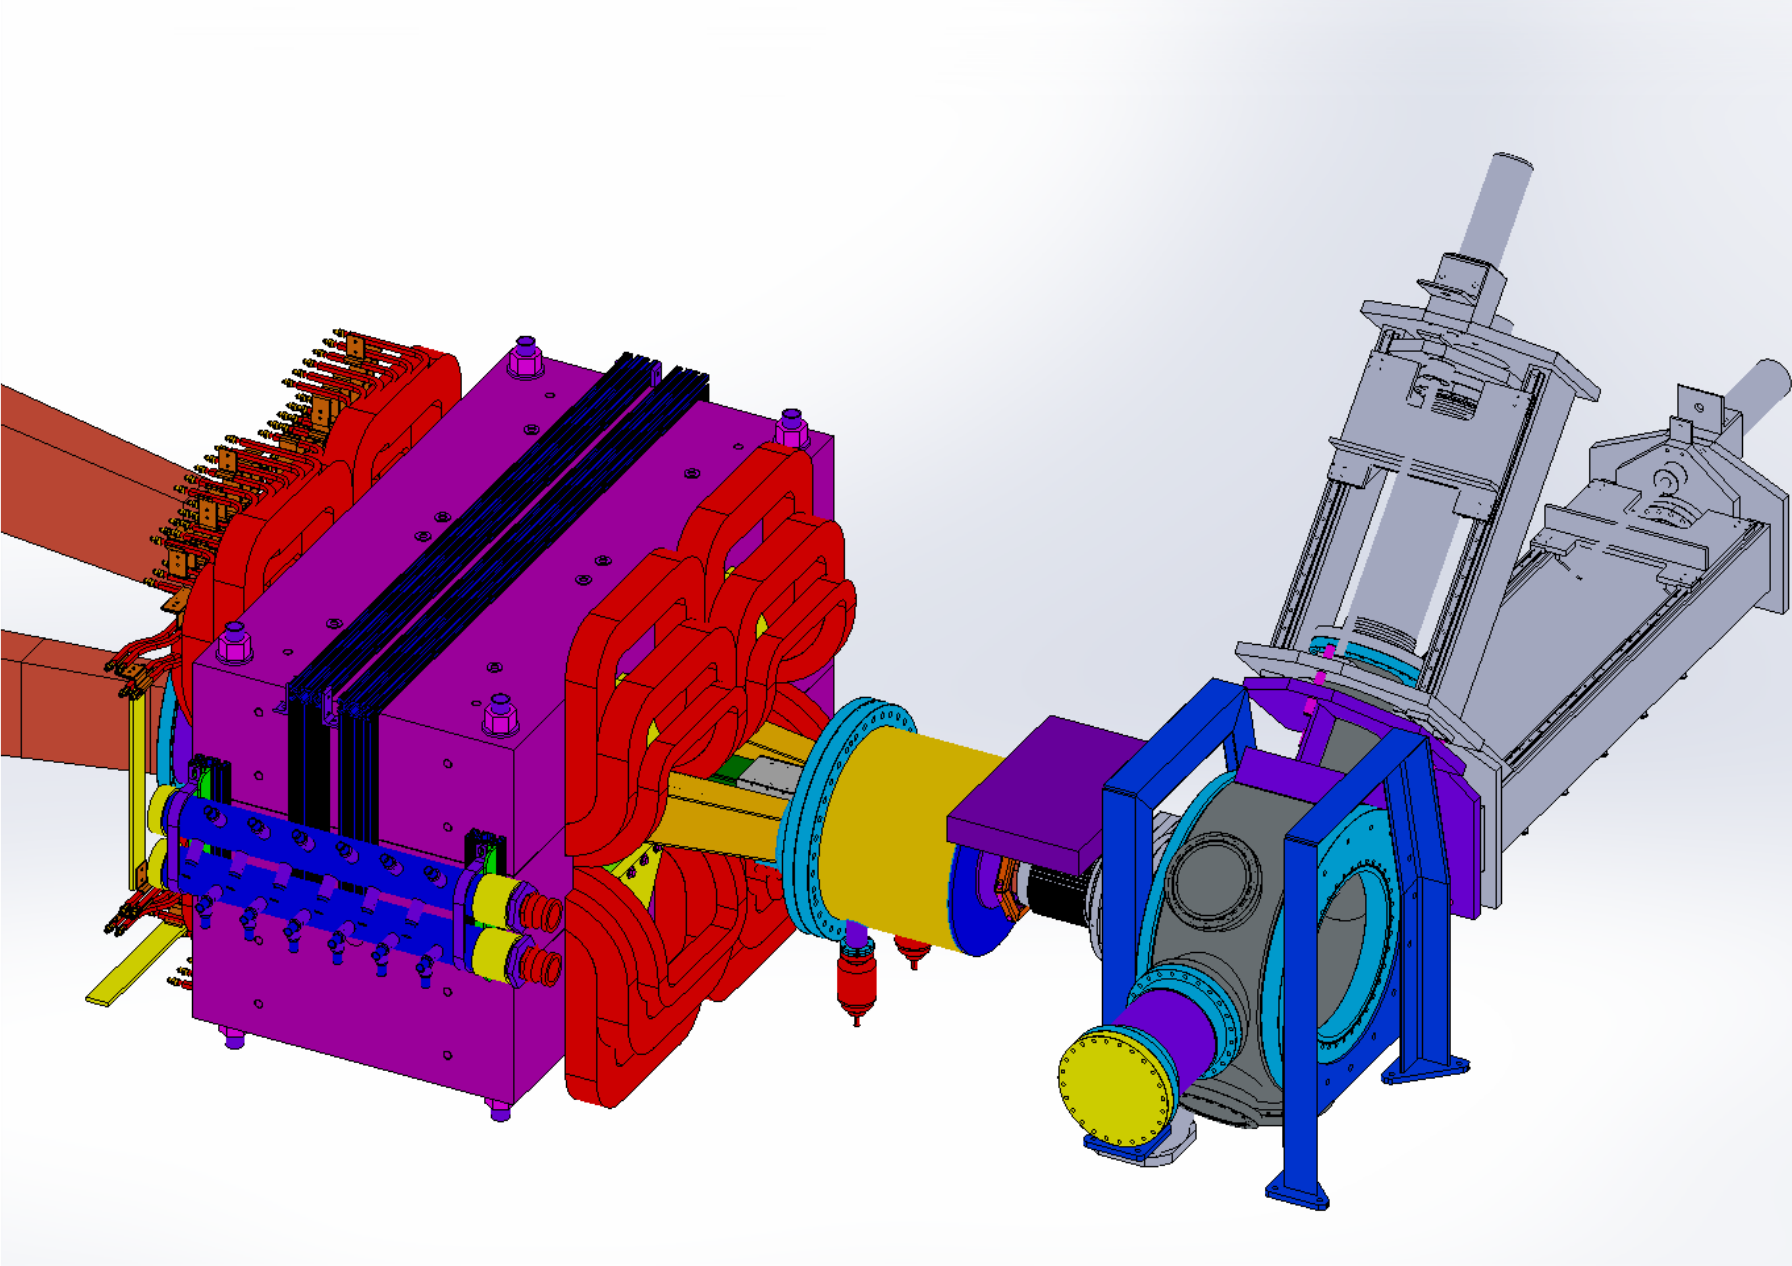
\includegraphics[width=\textwidth]{images/chap3/beam_line_target_pivot.png}
         \caption{beam target pivot}
         \label{Photo of CEBAF}
     \end{subfigure}
     \hfill
     \begin{subfigure}[b]{0.45\textwidth}
         \centering
         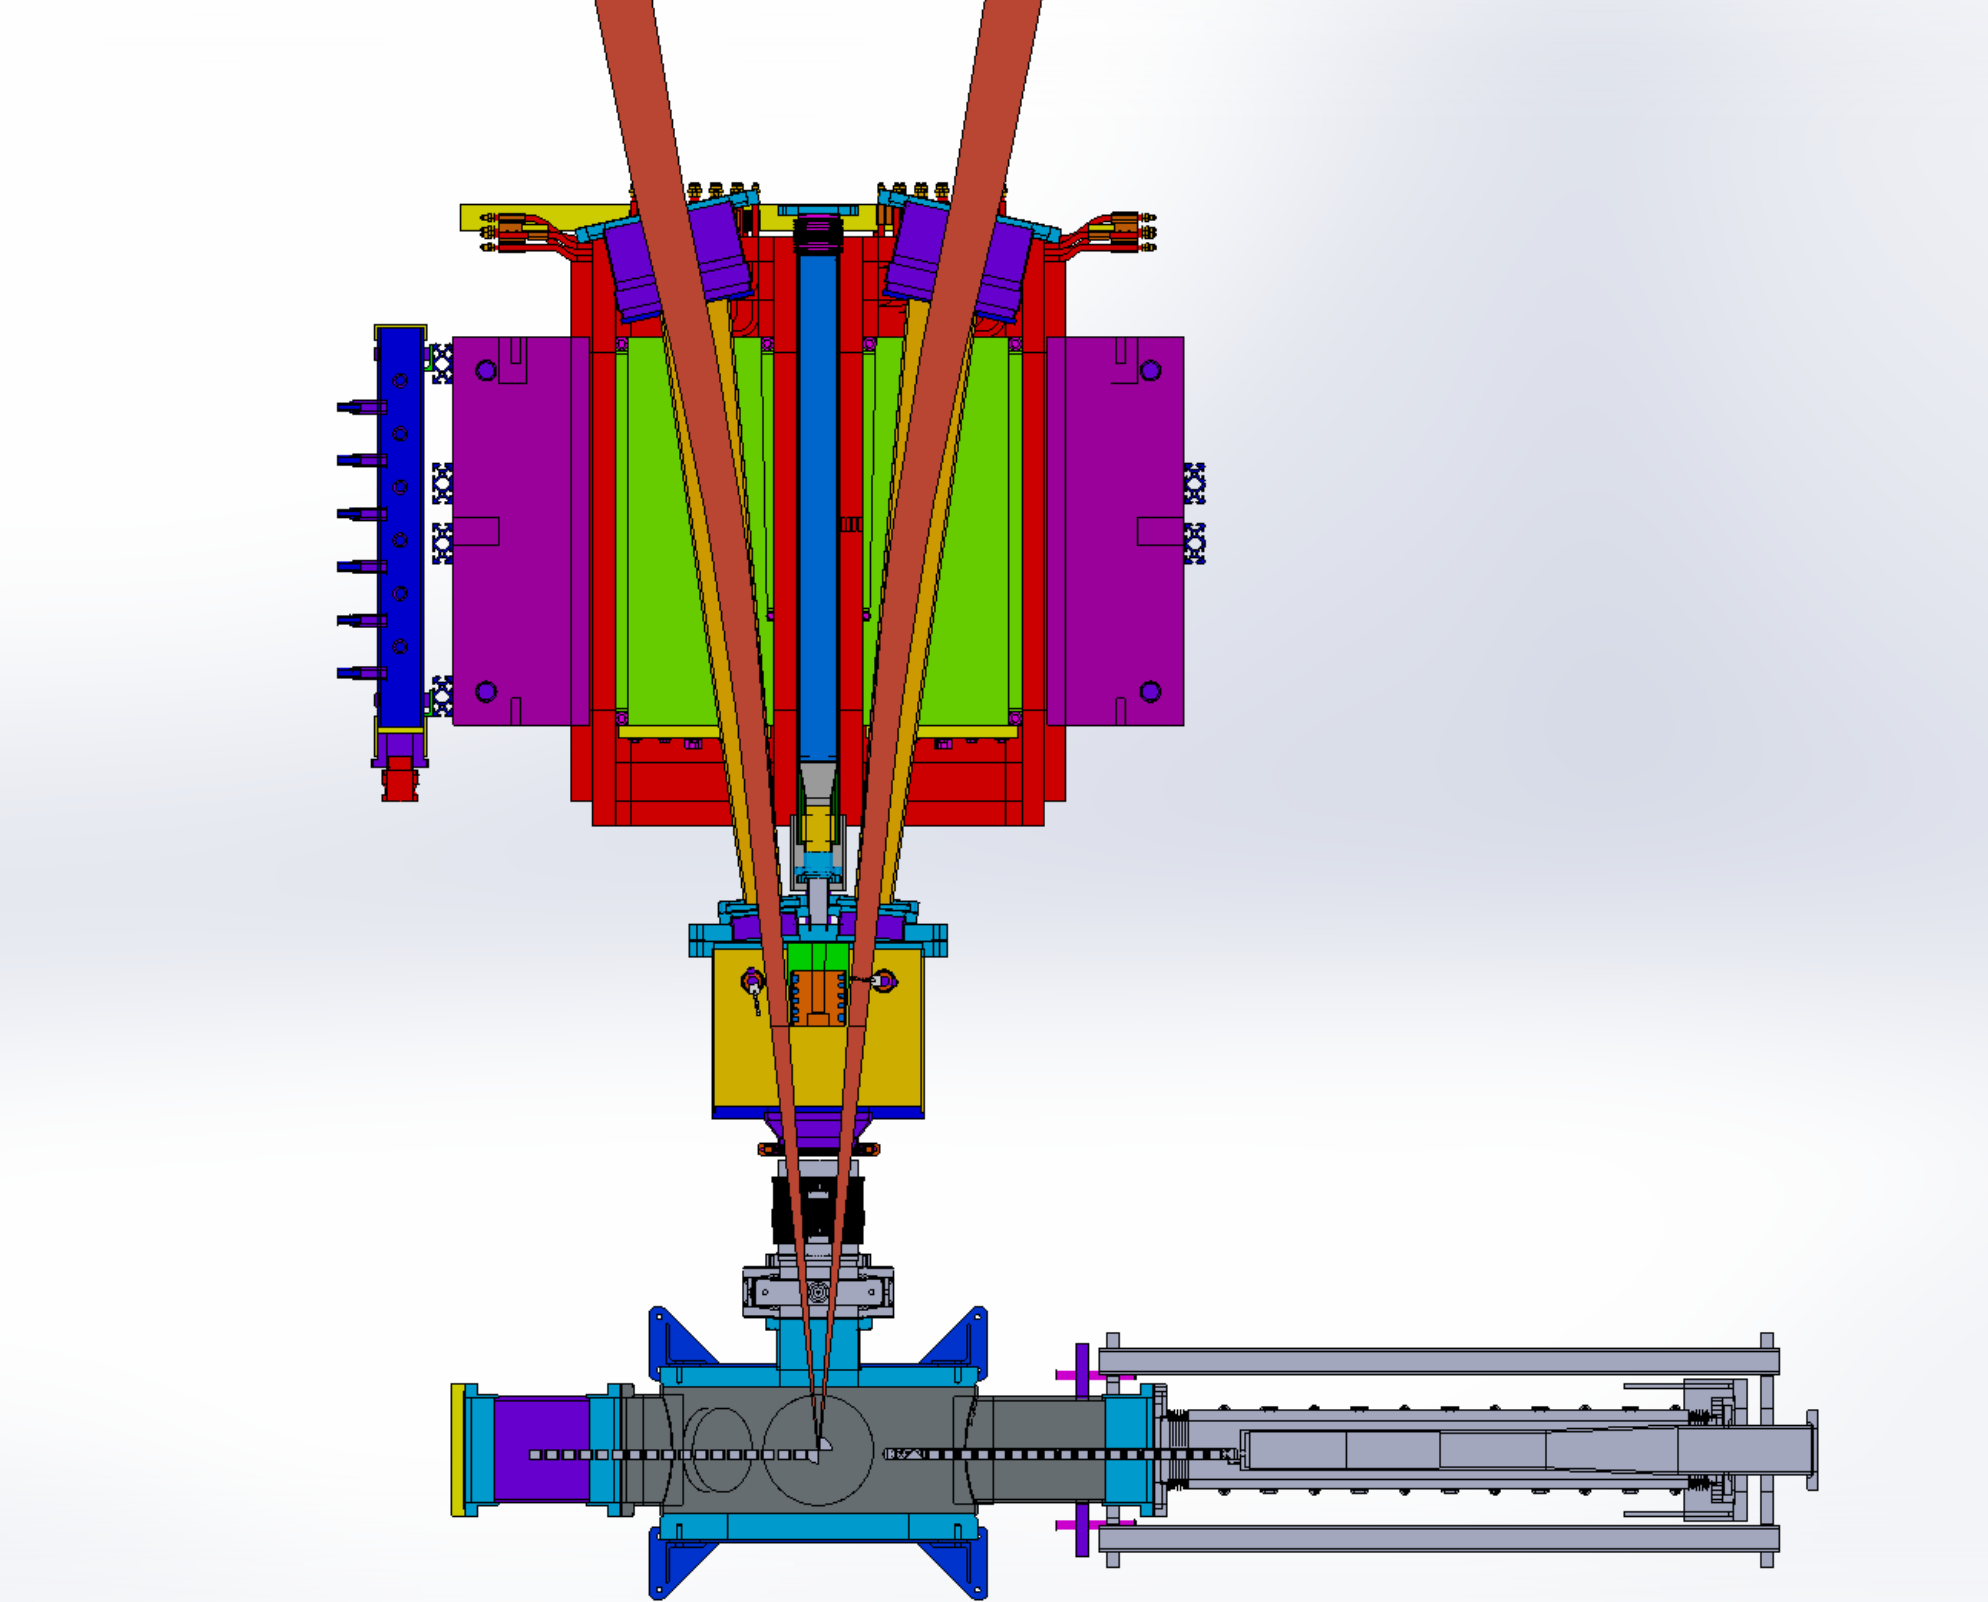
\includegraphics[width=\textwidth]{images/chap3/hrs_colli_corss_diag.png}
         \caption{disagr[from slides]}
         \label{gem_structure}
     \end{subfigure}
\end{figure}

\begin{figure}[!htbp]
    \centering
    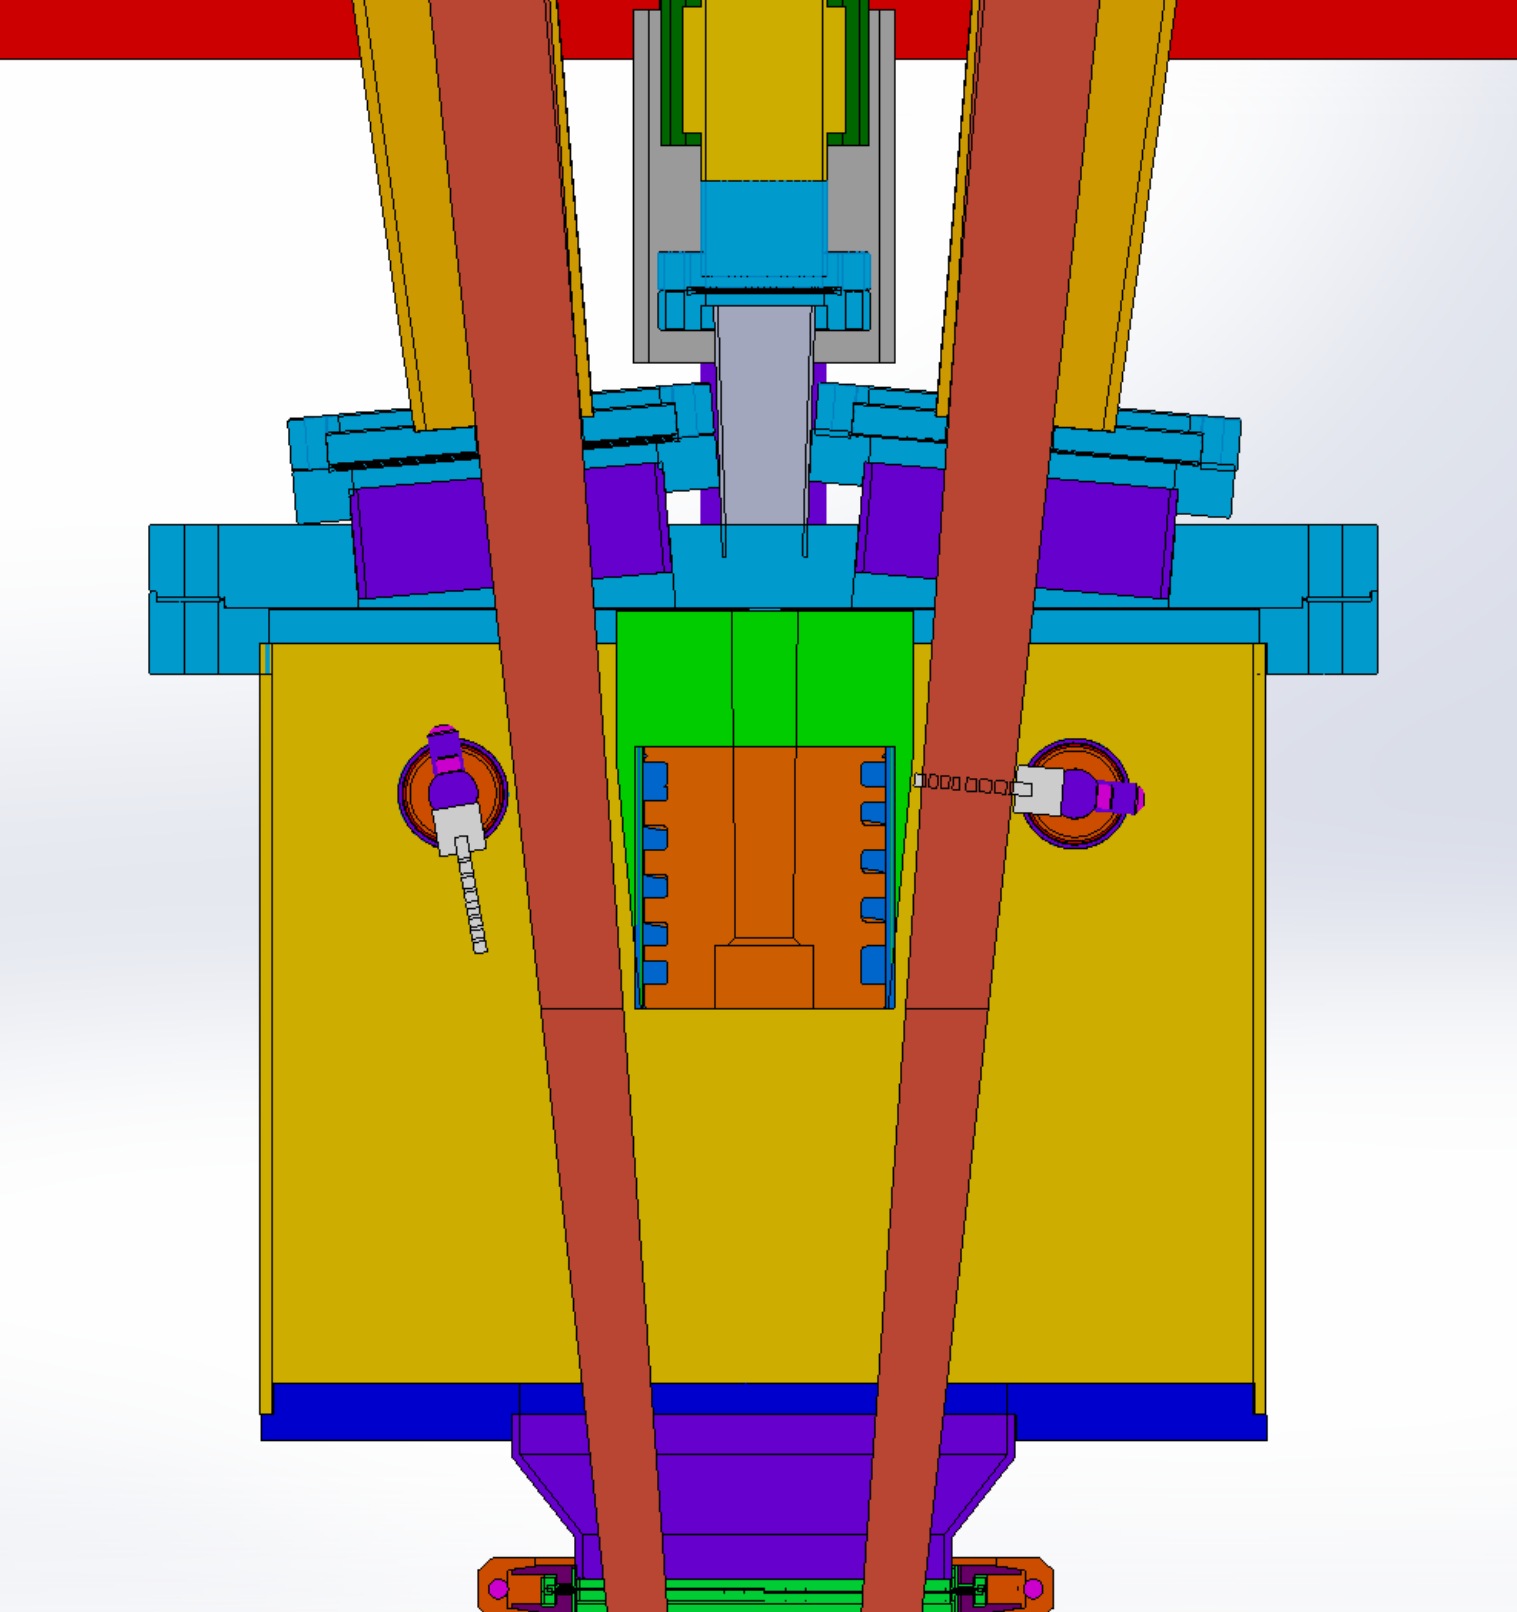
\includegraphics[width=0.8\textwidth]{images/chap3/hrs_pivot_detailed.png}
    \caption{detailed, need to add the labels}
    \label{fig:enter-label}
\end{figure}

\subsection{Sieve slit Collimators}

The sieve slit collimators used in Jefferson Lab's Hall A High Resolution Spectrometers (HRS) are 0.2-inch-thick tungsten plates, precisely drilled with a regular pattern of holes. Each hole measures 0.05 inches in diameter, except for three larger holes that are 0.106 inches across, which are utilized to aid in the accurate location of the collimator holes.
\begin{figure}[!htbp]
    \centering
    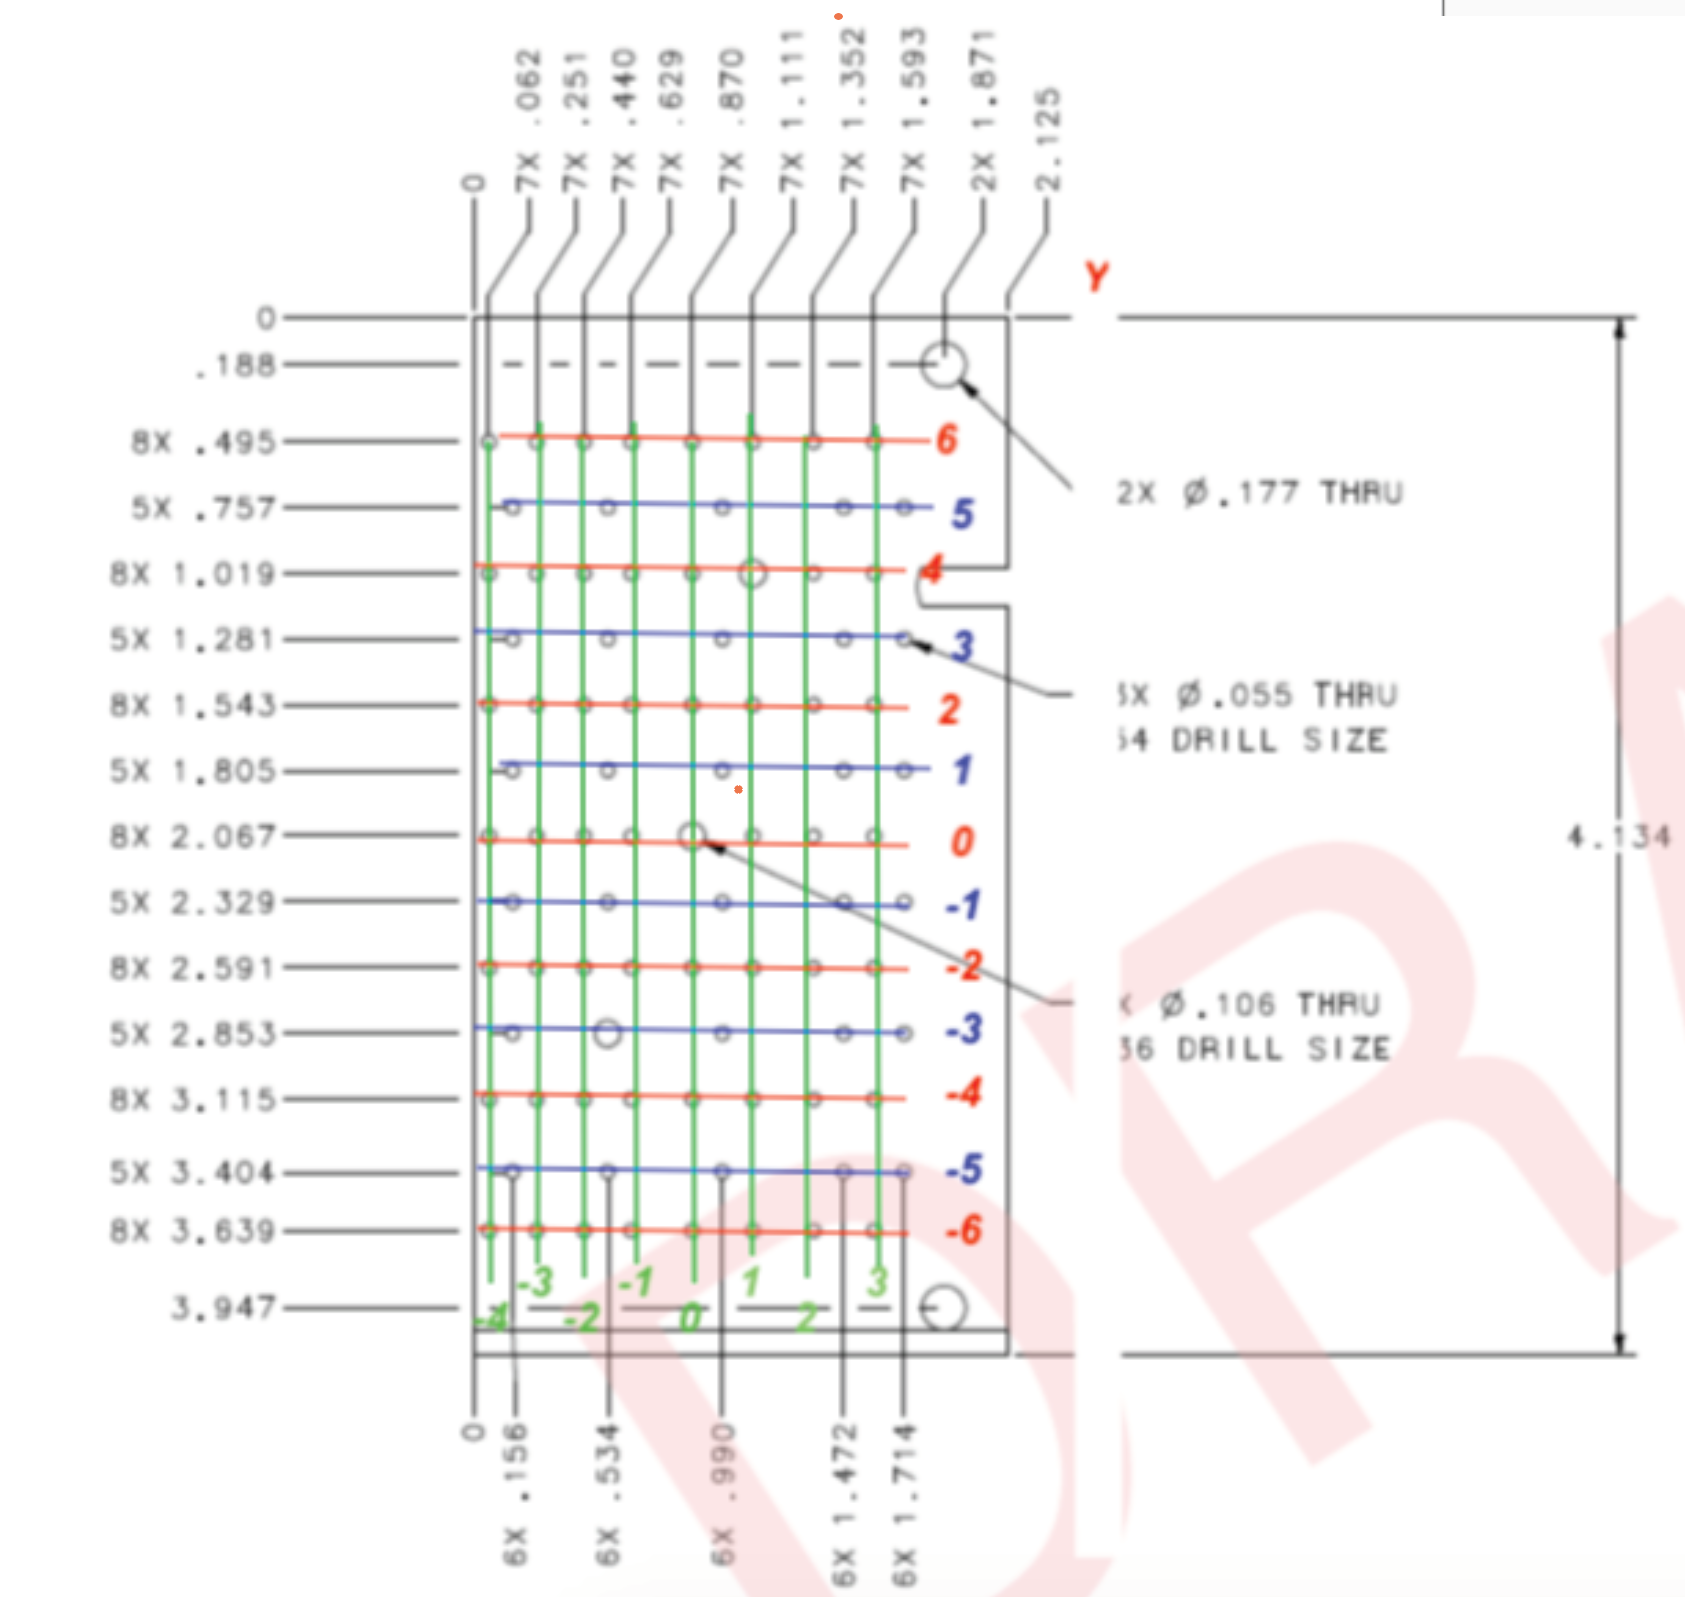
\includegraphics[width=0.8\textwidth]{images/chap3/sive_slit.png}
    \caption{Sieve slit used for PRex-II/CRex experiment [need to redraw]}
    \label{fig:enter-label}
\end{figure}
Each side of the HRS beamline is equipped with one sieve slit positioned at the beamline's entrance. The manufacture of these sieve slits involves high-precision Computer Numerical Control (CNC) machining and a thorough surveying process using laser technology, ensuring the utmost accuracy before the commencement of any experiment. The momentum of electrons passing through each sieve hole can be computed precisely, providing a robust reference for spectrometer calibration. Further details regarding the HRS calibration with sieve slits will be discussed in the subsequent chapter.

When the sieve slits are in place, only the electrons passing through these holes can reach the HRS. Each sieve slit is linked to a control unit, enabling manual placement or removal of the slit. During the production runs, the sieve is typically removed and only reinserted during optics runs. To ascertain the accuracy of this system, multiple optics runs were carried out throughout the experiment. 

\subsection{Magnet Chain of the HRS}

[ intro to be added]

\subsubsection{Septum Magnet}

The High-Resolution Spectrometers (HRS) in Jefferson Lab's Hall A possess a size constraint which establishes a minimum measurement angle of $12.5^\circ$. However, the requirements of the PREx-II and CREx experiments necessitate measurements to be conducted at an angle of $5^\circ$. To reconcile this discrepancy, a septum magnet is strategically placed between the collimator and the Q1 quadrupole magnet. This arrangement allows the septum magnet to pre-bend the scattered beam, thus aligning with the minimum angle constraint of the HRS.

\begin{figure}
    \centering
    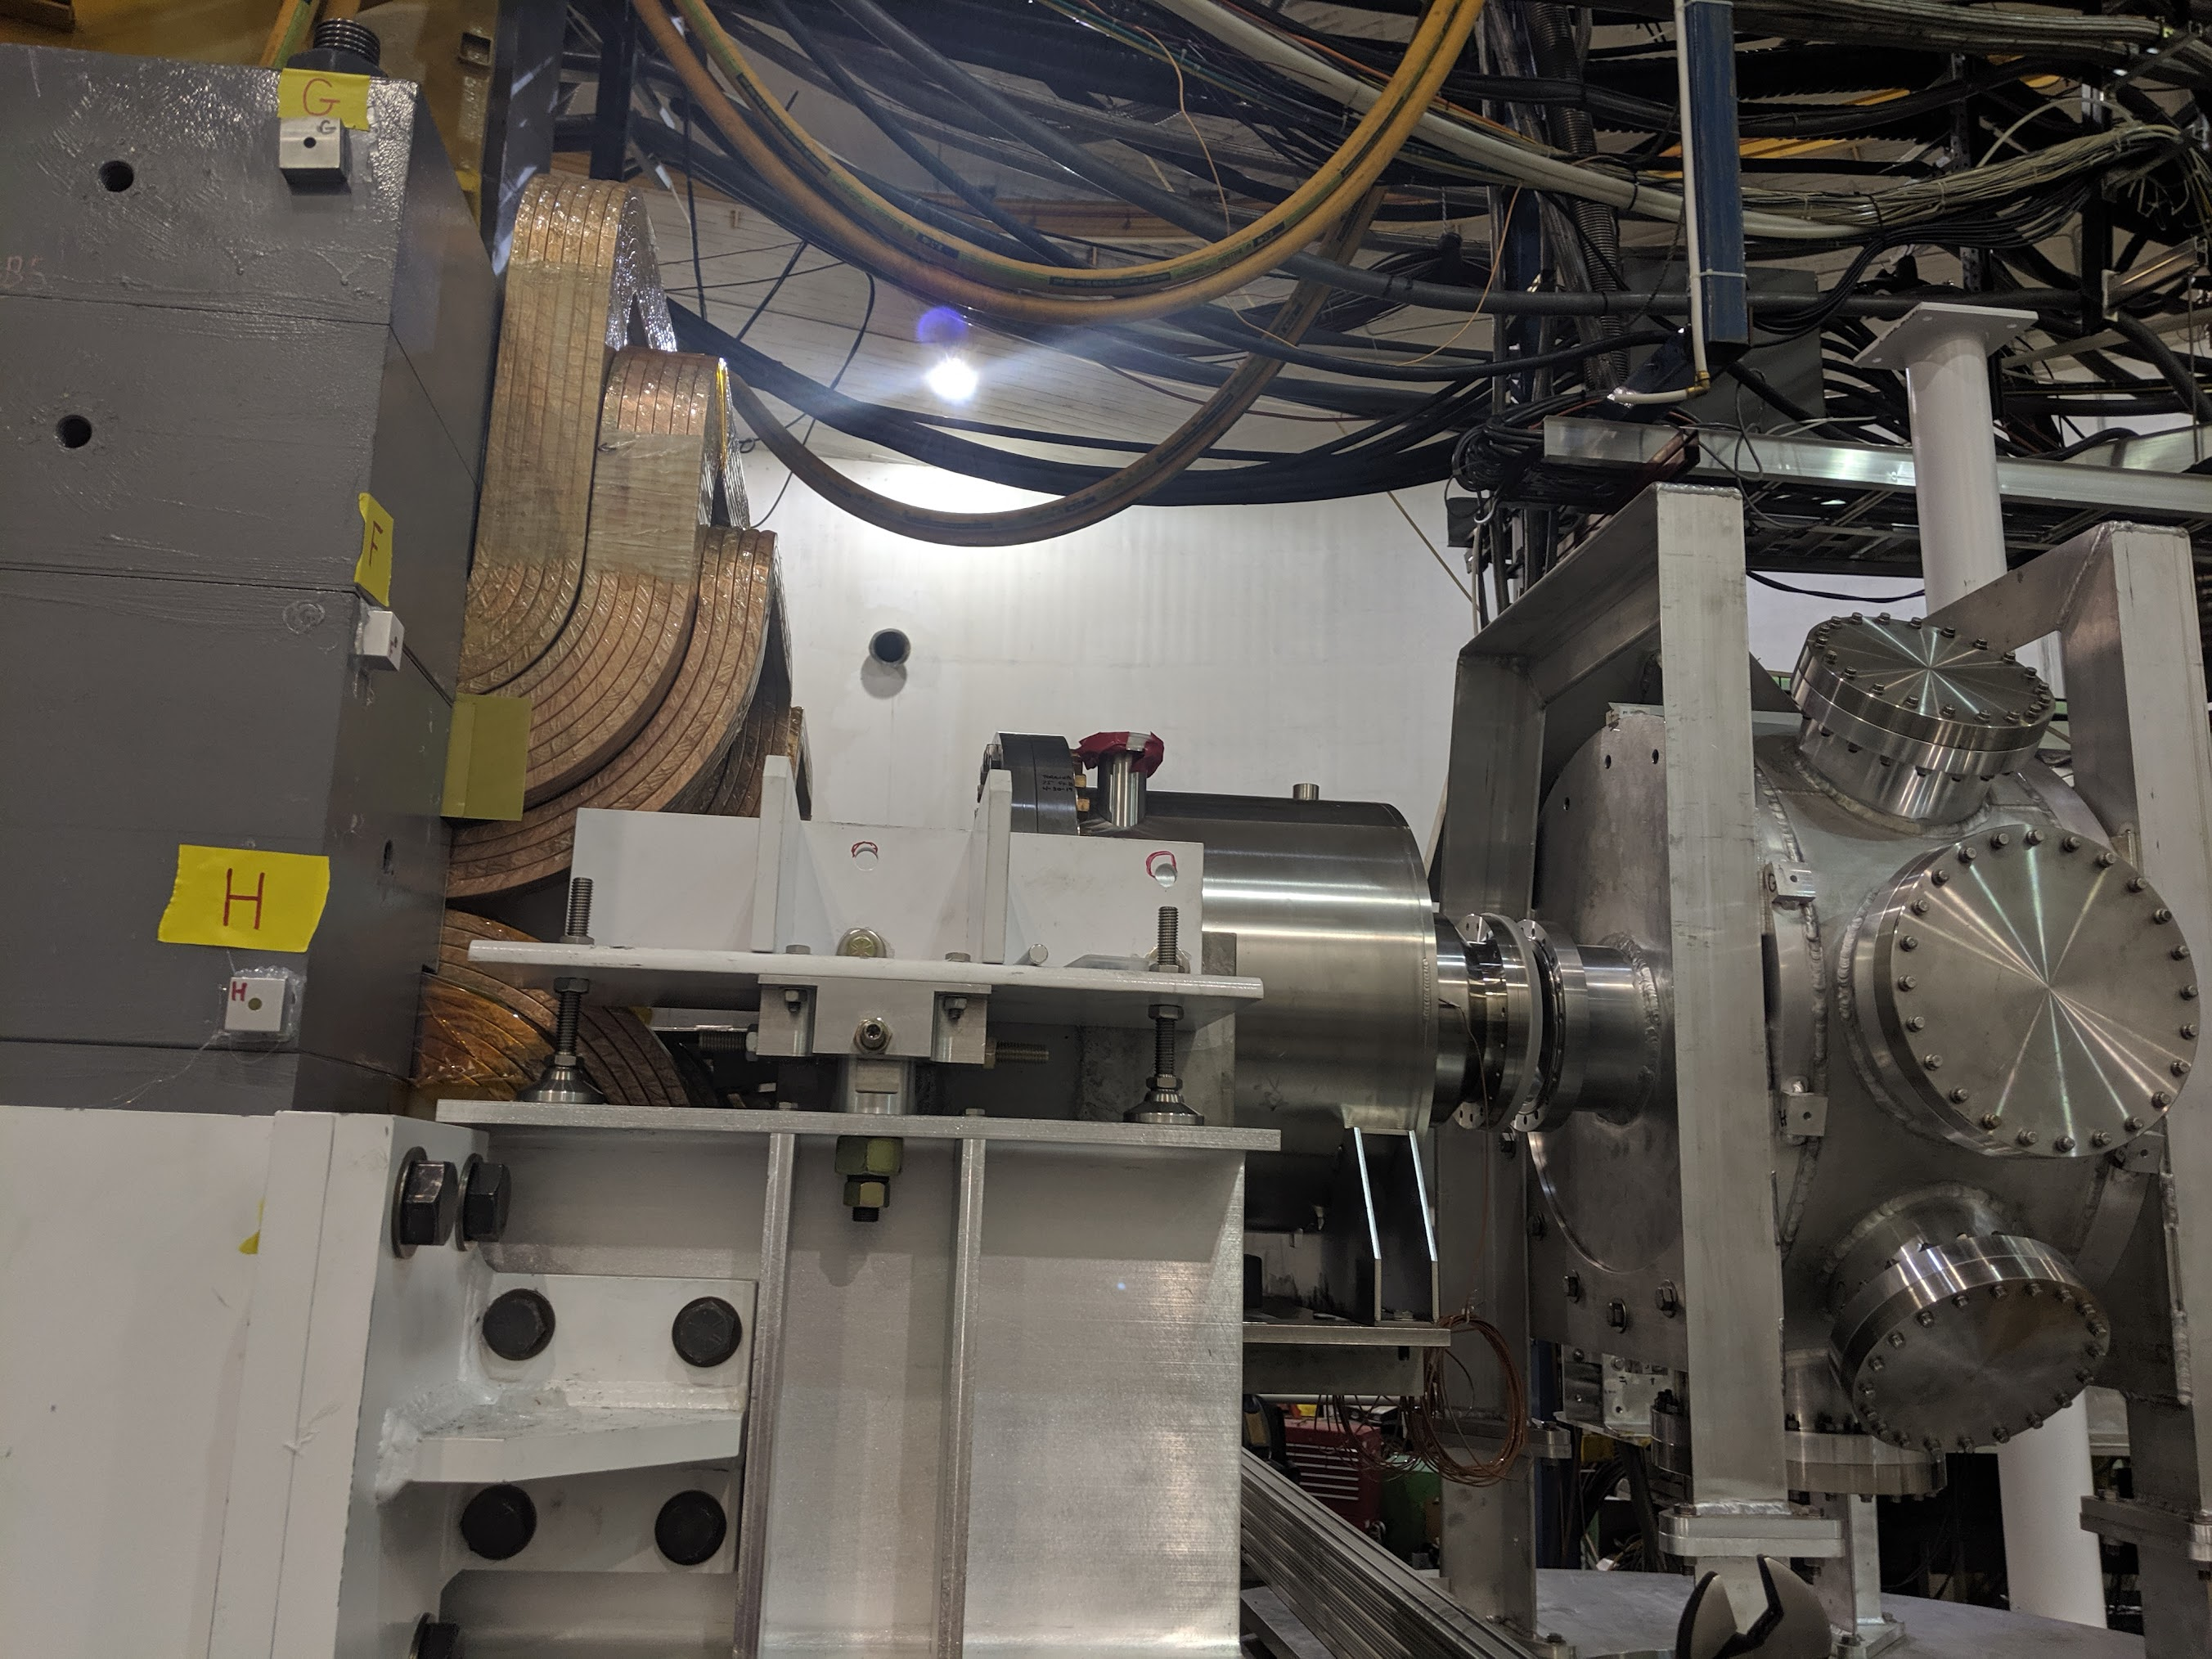
\includegraphics[width=0.8\textwidth]{images/chap3/septum_colli_targ_photo.jpg}
    \caption{Caption}
    \label{fig:enter-label}
\end{figure}

The septum magnet utilized in these experiments is a conventional, non-superconducting magnet. As depicted in the figure (to be added), the magnet is composed of coils positioned on the left and right beamlines. The magnetic field created by these coils is oriented vertically, causing the scattered electrons to be deflected towards the HRS while the unscattered beam continues along the central beamline towards the beam dump.

The Septum Magnet utilizes a 3-coil configuration, which offers two significant benefits. Firstly, it minimizes the vertical bore dimension, which is vital due to the confined spatial conditions. Secondly, this configuration reduces the coil current, which in turn decreases the thermal power relative to the required field integral. 


\subsubsection{QQDQ magnet package}

[from gpt, whether need to add?]

[.... plot, HRS QQDQ layout plot]

The High-Resolution Spectrometer (HRS) in Jefferson Lab's Hall A employs a quadrupole-quadrupole-dipole-quadrupole (QQDQ) magnetic configuration as the primary component of its particle tracking system.

The QQDQ magnetic package is designed to provide high-resolution momentum analysis and precise particle tracking, crucial for the HRS's function. It consists of two quadrupole magnets (Q1 and Q3), one dipole magnet (D), and another quadrupole magnet (Q2), arranged sequentially in the stated order.

The role of the quadrupole magnets is to focus the particle beam onto the plane of the detector. Specifically, the first and third quadrupole magnets (Q1 and Q3) act as vertical focusing lenses, while the second quadrupole magnet (Q2) serves as a horizontal focusing lens.

The dipole magnet (D) lies between the Q2 and Q3 quadrupoles. This magnet has a significant role in the QQDQ configuration as it deflects the particle beam through a particular angle, thereby separating the particles based on their momentum. This momentum dispersion feature of the dipole magnet allows the HRS to discern and analyze particles of differing momenta.

The unique combination of the quadrupoles and dipole in the QQDQ configuration grants the HRS excellent momentum resolution, precise trajectory determination, and a large angular acceptance. As such, this makes the Jefferson Lab's HRS an incredibly versatile and precise instrument for a wide range of nuclear physics experiments.

\begin{figure}
    \centering
    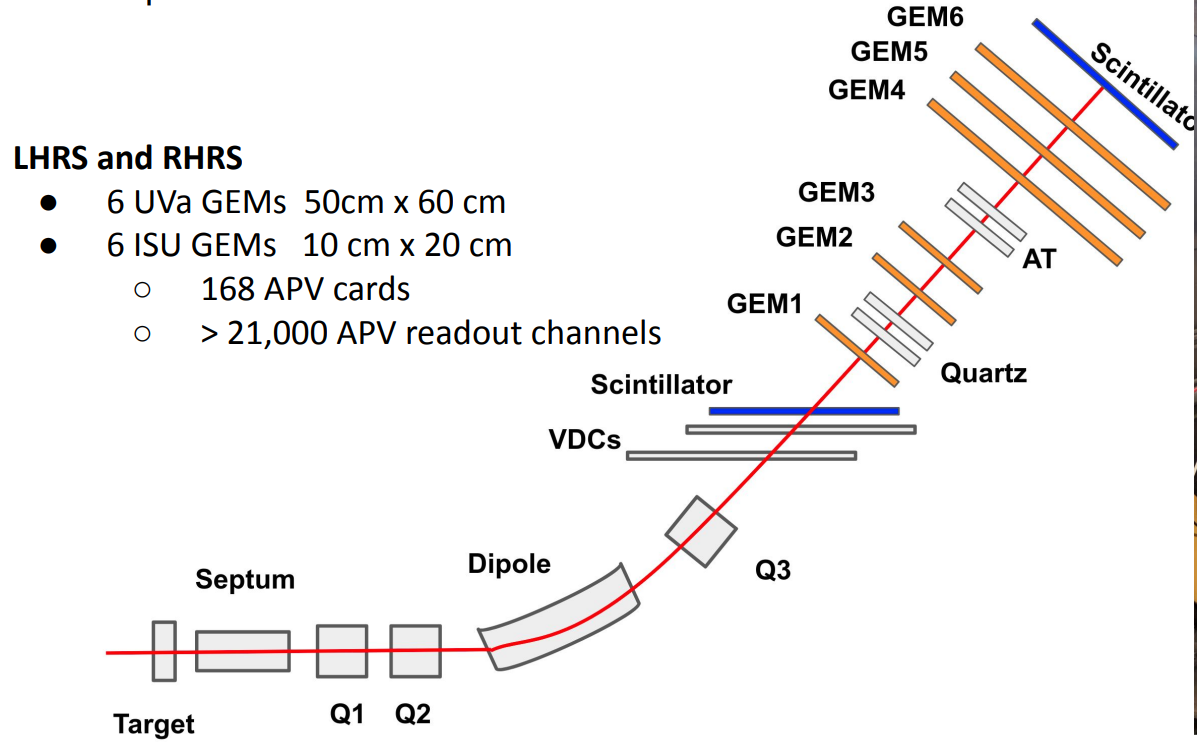
\includegraphics[width=0.8\textwidth]{images/chap5/gem_apparatus_in_hrs_2d.png}
    \caption{HRS QQDQ chain, to be replaced}
    \label{fig:enter-label}
\end{figure}

\subsection{detector package}

The detector package serves as a fundamental component of the spectrometer, specifically engineered for proficient particle detection, identification, and momentum assessment. It comprises an array of detection devices, each imparting unique capabilities, that collectively facilitate a thorough particle detection and analysis.

In the context of the PRex-II/CRex experiment, the detector package incorporates S0 and S3 scintillators. These provide trigger mechanisms for the counting mode of Data Acquisition, enabling efficient event recording. The Vertical Drift Chambers are included for precise particle tracking, facilitating the determination of particle trajectories within the spectrometer. Quartz integrating detectors is the main detector used in production mode to measure the parity violation asymmetry. Gas Electron Multiplier (GEM) detectors are integrated into the package, supplementing the tracking capacities of the detector assembly. 

\subsection{Vertical Drift Chamber}

The Vertical Drift Chambers (VDCs) play a pivotal role in discerning the trajectory of particles observed within the spectrometer. Constructed as multi-wire proportional chambers, these VDCs offer meticulous assessments of both the position and angles of the charged particles traversing them. Each VDC within the HRS is generally composed of two wire planes, set at an angle relative to one another. This strategic arrangement facilitates the accurate determination of a charged particle's two-dimensional position as it moves through the chamber.

Additionally, the use of two chambers enables the VDCs to deliver comprehensive spatial data, including the position $(x,y)$ and orientation $(\theta, \phi)$ of the particle. This wealth of information makes possible the intricate measurement of the kinematics of the scattered electrons.

A more in-depth exploration of the VDC, and the process of reconstructing kinematic data based on VDC measurements, will be provided in Chapter 4. This elaboration will further illuminate the essential role these devices play within the experimental apparatus.

\begin{itemize}
    \item structure of the VDC 
    \item readout electronics (to be added, move to chapter 4)
\end{itemize}

\subsection{S0, S3 scintillator}

The PRex-II/CRex experiment incorporates two scintillator packages, labeled S0 and S3, in each High-Resolution Spectrometer (HRS). These packages furnish triggers for the counting mode of Data Acquisition (DAQ), a critical function in optics calibration, $Q^2$ measurements, and Spot++ routines.

The first scintillator package contains two scintillators, S0, is strategically positioned between the Vertical Drift Chambers (VDC) and the Gas Electron Multiplier (GEM) detectors, enabling the initial phase of particle detection.

The second scintillator package, S3, comprises three plastic scintillator paddles. It is situated above the GEM detectors and is oriented at a $45^\circ$ angle. This placement is perpendicular to the scattered beamline. 


\subsection{Quartz detectors and AT detectors}



\subsection{GEM detector}

In the PRex-II experiment, 6 GEM detectors are installed in each HRS to provide supplemental tracking capability. 12 GEM detectors are used in total in the experiment. Half of them are GEM detectors with size of $20\times 10$ centimeter manufactured in IDU, and half of the GEM detectors with the size of $60\times 50$ centimeters are manufactured in the University of Virginia design for Super BigBite Experiment which performance in 2022. The PRex experiment provides a unique opportunity to test the GEM detectors in the real experimental environment before the SBS experiment. In the next section, we will introduce more about the GEM detectors and their DAQ systems. 

In the CRex experiment, to reduce the scattering caused by the GEM detector, two(check check??) of the IDU GEM detector are removed from the data acquisition. 


\section{GEM detector for the PRex/CRex experiment}

Gas Electron Multiplier (GEM) detectors are an important type of detector used in high-energy physics and various other fields for detecting charged particles, X-rays, and other ionizing radiation. The GEM detector was invented by Fabio Sauli at CERN in 1997 and has since become a crucial tool in the field of particle physics.

The GEM detector operates based on the principle of gas ionization and subsequent avalanche multiplication. It is essentially a thin, metal-clad polymer foil chemically pierced by a high density of holes. This foil is typically sandwiched between two electrode plates. When a voltage is applied across the electrodes, an electric field is generated in the holes, resulting in strong gas amplification of the ionization electrons produced in the detector gas by the traversing radiation.

When a charged particle passes through the detector, it ionizes the gas atoms, generating primary ion-electron pairs. These electrons are then drifted toward the GEM foils due to the electric field. When they enter the high-field region within the holes of the GEM foil, they trigger an avalanche multiplication, leading to a significant increase in the number of electrons.

\begin{figure}
     \centering
     \begin{subfigure}[b]{0.45\textwidth}
         \centering
         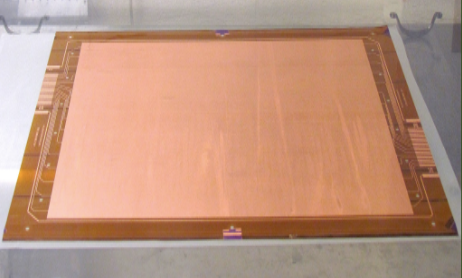
\includegraphics[width=\textwidth]{images/chap3/gem_foil_photo.png}
         \caption{Photo of GEM}
         \label{Photo of CEBAF}
     \end{subfigure}
     \hfill
     \begin{subfigure}[b]{0.45\textwidth}
         \centering
         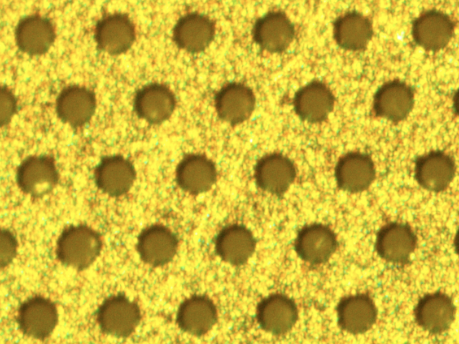
\includegraphics[width=\textwidth]{images/chap3/gem_foil_micro.png}
         \caption{JLAB GEM to be replaced}
         \label{gem_structure}
     \end{subfigure}
\end{figure}

[ plot ..... GEM detector Garfield Simulation EM field plot, my master thesis]

This multiplication process occurs in a confined geometry, reducing the likelihood of photon-mediated feedback and increasing the detector's gain, rate capability, and stability. The resulting electron avalanche then induces a signal on the readout electrode, which can be processed to give the position and amount of ionizing radiation.

GEM detectors are known for their high spatial resolution, good time resolution, and capability of handling high particle rates, making them an ideal choice for many experiments. Furthermore, they are robust, non-ageing, and relatively easy to construct and operate, making them a practical choice for many applications.

In the PRex-II experiment, each HRS have 6 GEM detectors, three of them are UVa GEM detector made for Super bigBite Experiment with active area of $60\times 50$ centimeter, the rest three GEM detector are made in Idohle University with area of $20 \times 10$ centimeters. All the 6 GEM detector can detector particle separately and with the 6 GEM detectors it could pride high accurate tracking of the particles in the spectrometer.  

[ plot, GEM detector installation in the detector hub]
\begin{figure}
    \centering
    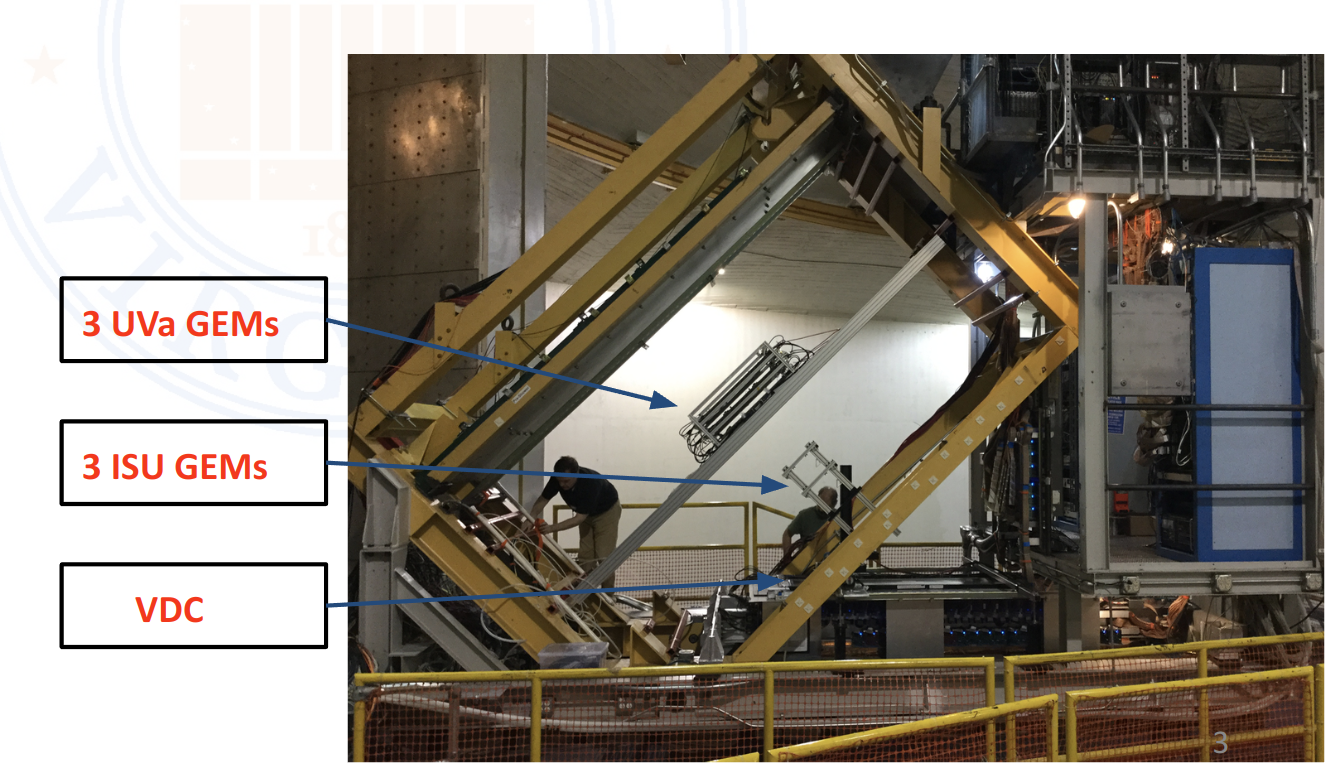
\includegraphics[width=0.8\textwidth]{images/chap3/gem_in_hrs.png}
    \caption{Caption}
    \label{fig:enter-label}
\end{figure}

\subsection{GEM detector Structure}

The GEM detectors are constructed with a layered design to ensure sufficient electron amplification. As illustrated in Figure [ref], Below the three layers of GEM foil, readout strips are secured to a honeycomb board. The use of a honeycomb structure minimizes the material present in the beamline, thus reducing its influence on scattered electrons and lessening potential noise.

Underneath the honeycomb board, there exists an additional chamber circulating air to prevent the board from warping. Above the three layers of GEM foil, a cathode is installed. This cathode is covered with a single layer of copper-coated polyimide that connects it to the high-voltage power supply.

The cathode layer is covered by a polyimide window. Positioned above it, an aluminum-coated layer is installed. This layer is connected to the same high voltage as the cathode. This design will depolarize the polyimide window. Through this detailed structure, the GEM detectors ensure efficient detection and measurement of charged particles.


\begin{figure}
     \centering
     \begin{subfigure}[b]{0.2\textwidth}
         \centering
         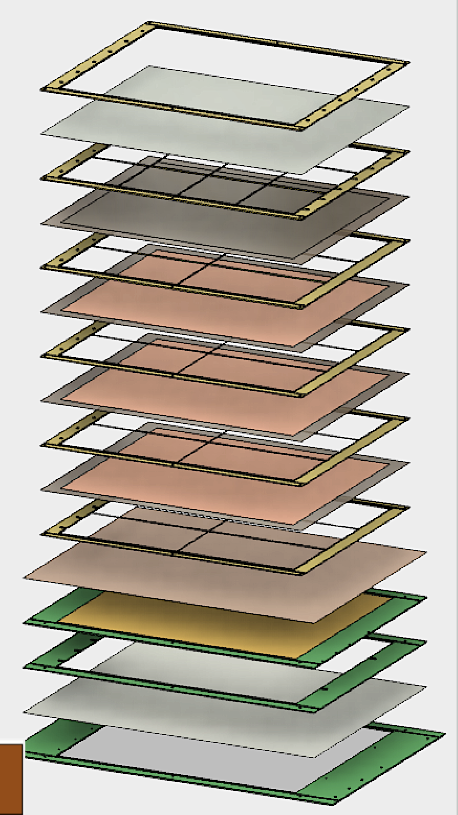
\includegraphics[width=\textwidth]{images/chap3/gem_structure.png}
         \caption{Photo of GEM [to be replaced]}
         \label{Photo of CEBAF}
     \end{subfigure}
     \hfill
     \begin{subfigure}[b]{0.45\textwidth}
         \centering
         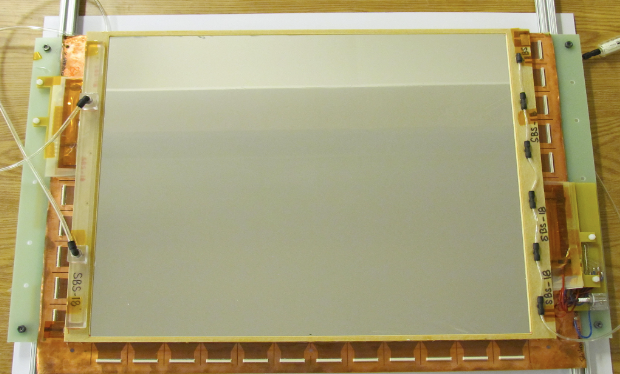
\includegraphics[width=\textwidth]{images/chap3/gem_chamber.png}
         \caption{JLAB GEM to be replaced}
         \label{gem_structure}
     \end{subfigure}
\end{figure}

\subsection{GEM detector High Voltage}

The voltages applied to the GEM foils are regulated by resistor chains. Figure [ref] depicts the specific resistors utilized in the PRex/CRex experiment. The depolarizing window at the top of the GEM chamber shares the same high voltage as the cathode layer. The voltage at the top of the GEM detector is slightly higher than that at the bottom because there are fewer avalanche electrons at the top. This voltage distribution helps to protect the GEMs from potential damage.

Each of the GEM detectors is safeguarded by resistors of $10M\Omega$ to limit the current passing through the GEM. This precautionary measure helps to prevent short circuits or the occurrence of a large drift current within the GEM, ensuring the overall safety and performance of the detector.


\begin{figure}
    \centering
    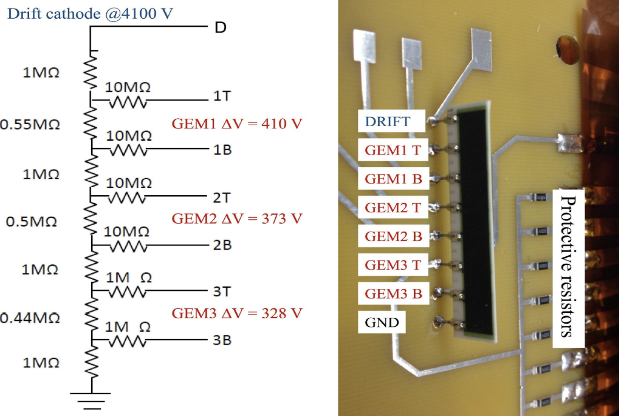
\includegraphics[width=\textwidth]{images/chap3/GEM_register_chain.png}
    \caption{Caption}
    \label{fig:enter-label}
\end{figure}


The high voltage is powered with two CEAN high voltage modules. Each module has 8 channels, 6 of which are used to power the GEM detectors, each GEM detector is connected to one high voltage channel.  Both of the modules can be controlled remotely in the counting-house. 

\begin{figure}[!htbp]
    \centering
    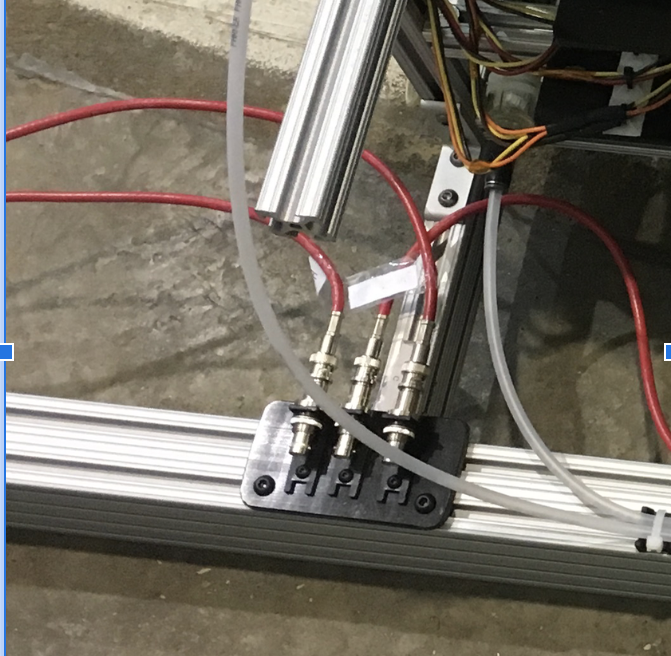
\includegraphics[width=0.45\textwidth]{images/chap3/gem_hv_connector.png}
    \caption{Caption}
    \label{fig:enter-label}
\end{figure}

[GEM .... GEM detector HV module]


The operational voltage of the GEM detector is selected as the lowest possible voltage that still fulfills the experimental efficiency requirements. When the high voltage is elevated, the potential within the GEM holes increases, which leads to a larger number of avalanche electrons and subsequently higher detection efficiency. However, a higher voltage also elevates the risk of GEM trips, which can potentially damage the GEM detector.

On the contrary, a lower high voltage leads to diminished efficiency. The operational voltage is thus chosen based on the results of a high-voltage scan. This scan evaluates the efficiency of the GEM detector across a range of high voltages to identify the optimal operating condition that balances efficiency and the safety of the device.

[GEM detector efficiency scan]

\subsection{Gas Flow}

In the Gas Electron Multiplier (GEM) detector, the working gas is a mixture of Argon (Ar) and Carbon Dioxide (CO2) in a proportion of 75:25. The primary component, Argon, serves as the ionization medium. Incident radiation interacts with the Argon atoms upon entering the detector, ionizing them and liberating electrons. To prevent the formation of Argon ions after the initial ionization process, which could cause distortions in the electric field, Carbon Dioxide is included in the mixture. As an electronegative gas, CO2 captures and neutralizes these ions, mitigating potential field distortions.

The gas supply is managed via the Hall A gas system. After passing through the gauge valve, the gas is divided into six channels and directed to a bubbler. Post-bubbler, the gas proceeds through a dehumidifier valve before being fed into the GEM chambers. This process ensures an optimal, controlled gas environment within the detectors for precise experimental conditions.

\subsection{GEM detector Readout Electronics}

The GEM detector used in the PRex-II/CRex experiment utilizes a strip readout method. Following the amplification cascade, the electrons are collected by readout strips. Each of these strips is directly linked to a charge-sensitive frontend amplifier. Subsequently, the signals are transformed into LVDS (Low-Voltage Differential Signaling) format and dispatched to a digitizer, where they are converted into digital signals. A schematic diagram of the readout electronics is shown in Figure [ref]. The upcoming sections will offer an in-depth description of each part of the electronics system.

[... to be added, add the readout electronics diagram]

\subsubsection{Front End}

[... to be added, GEM detector with APV]

The GEM detector utilizes APV25, a low-noise charge-sensitive preamplifier for readout operations\cite{Jones:1069892,Jones:432224}. Initially designed for reading silicon microstrip detectors in the CMS tracker at the LHC, APV25 is a 128-channel analogue pipeline chip. Each channel consists of a low-noise amplifier, a 192-cell analogue pipeline, and a deconvolution readout circuit. Data output is transmitted via a single differential current output through an analogue multiplexer.

The dimensions of the GEM detectors are 60 cm by 50 cm. The longer side, equipped with 1536 channels, is read out by twelve APV25 cards. All twelve cards are connected to a single 12-slot backplane that provides power, control, and readout functionality to the APV25. On the other hand, the shorter side, with 1280 channels, is read out by ten APV25 cards. These cards are linked to two 5-slot backplanes. The APV25 is powered by a low voltage regulator that can provide 2.5V and 1.25V to energize the APV25 frontend cards.

Two distinct patch panels are utilized within the data acquisition (DAQ) system. The digital patch panel serves the purpose of distributing digital signals to two different backplanes. On the other hand, the analog patch panel is specifically designed to convert a 5-channel HDMI signal into a 4-channel HDMI signal. This conversion is essential to facilitate the signal's compatibility with the MPD.


[... fig, cooling] \\

[... fif, GEM with APV]


\subsubsection{MPD and Data Transfer}

The Multi-Purpose Digitizer (MPD) board is designed to seamlessly manage up to 16 APV front-end cards. It reads out the associated analog data streams and transmits both the control and configuration signals. Each MPD comes with 4 analog HDMI input ports, each capable of digitizing 4 APV front-end cards (128 channels). The MPD can sample the signal at a rate of 40MHz. After digitization, the signals are forwarded to [??? figure name?] before being transferred to the database. (This needs to be double-checked.)

\section{production DAQ system}


\chapter{Data Analysis}

PRex-II Experiment was operated on Jefferson Lab High-Resolution Spectrometer(JLab). The kinematics of the scattered electrons have to be measured on the Vertical Drift Chambers which are installed after the magnetic chains. All the measurements have to be converted back to the target coordination system in order to get the result. This chapter will discuss the detail of JLab HRS calibration, the calculation of the 4-momentum transfer square, and the GEM detector analysis. 

\section{Vertical Drift Chamber $T_0$ calibration}

\subsection{correction the initial drift time $T_0$}

Each HRS spectrometer is equipped with a package of four Vertical Drift Chambers (VDCs) that are oriented in the UV direction. The VDCs are filled with Argon (Ar) and flammable ethane, which is bubbled through alcohol. The gas filling is routed and delivered using the Hall A Gas System. Each wire in the VDCs is connected to a 3.5 kV high-voltage source.

[The electronics of the VDC, TO BE ADDED]

When a charged particle passes through the VDC chamber, it ionizes the gas atoms, creating a trail of ionized electrons along its path. The ionized electrons drift along the electric field lines due to the high voltage between the high voltage plane and signal wires. This ionization produces a pulse on the signal wires. Each VDC chamber contains 368 wires, and each wire is connected to a pre-amplifier. The amplified pulse signal is then passed through a discriminator and used to trigger the Time-Digital Converter (TDC). The TDC is stopped by the Hall overall event trigger.

After the particle trespass into the chamber, normally it will fire a cluster that contains 4-6 wires. As shown in Fig \ref{fig:vdc_wire_ionization_cluster}, the cross point between the trajectory of the particle and the VDC plane could be measured by measuring the drift distance between each wire. The drift distance is measured with the drift time that gets from the Time-Digital-converter. An accurate start time would be critical to get an accurate drift distance to get an accurate position on VDC.  If the threshold is set too high or too low, the VDC drift distance would be biased. An example of an improper setting of $T_0$ is shown in the plot, where a large number of 'wire shadows' can be observed. These shadows are caused by measurement bias.

[add more detail of the the ADC plot]

\begin{figure}
    \centering
    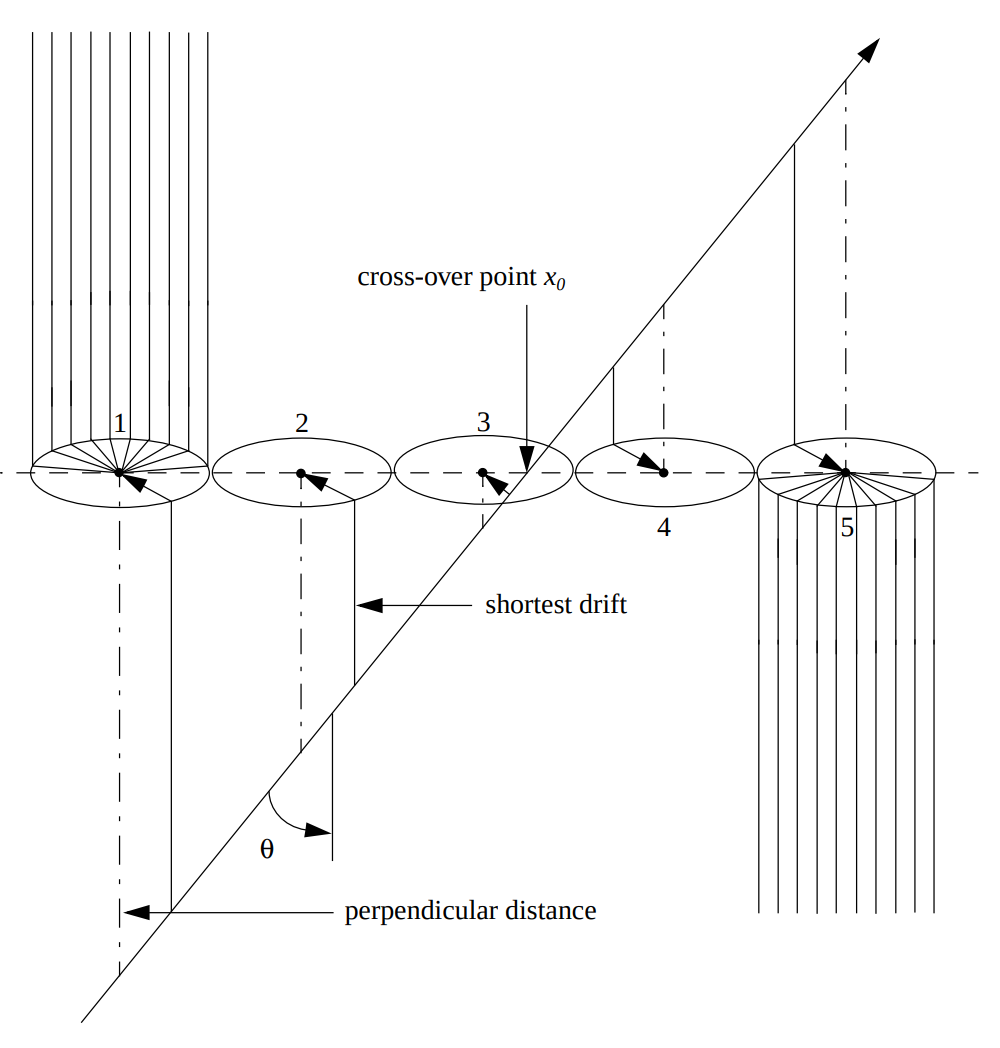
\includegraphics[scale = 0.25]{images/chap4/vdc_wire_ionize.png}
    \caption{Vertical Drift Chamber Ionization (need to redraw)}
    \label{fig:vdc_wire_ionization_cluster}
\end{figure}

\begin{figure}
    \centering
    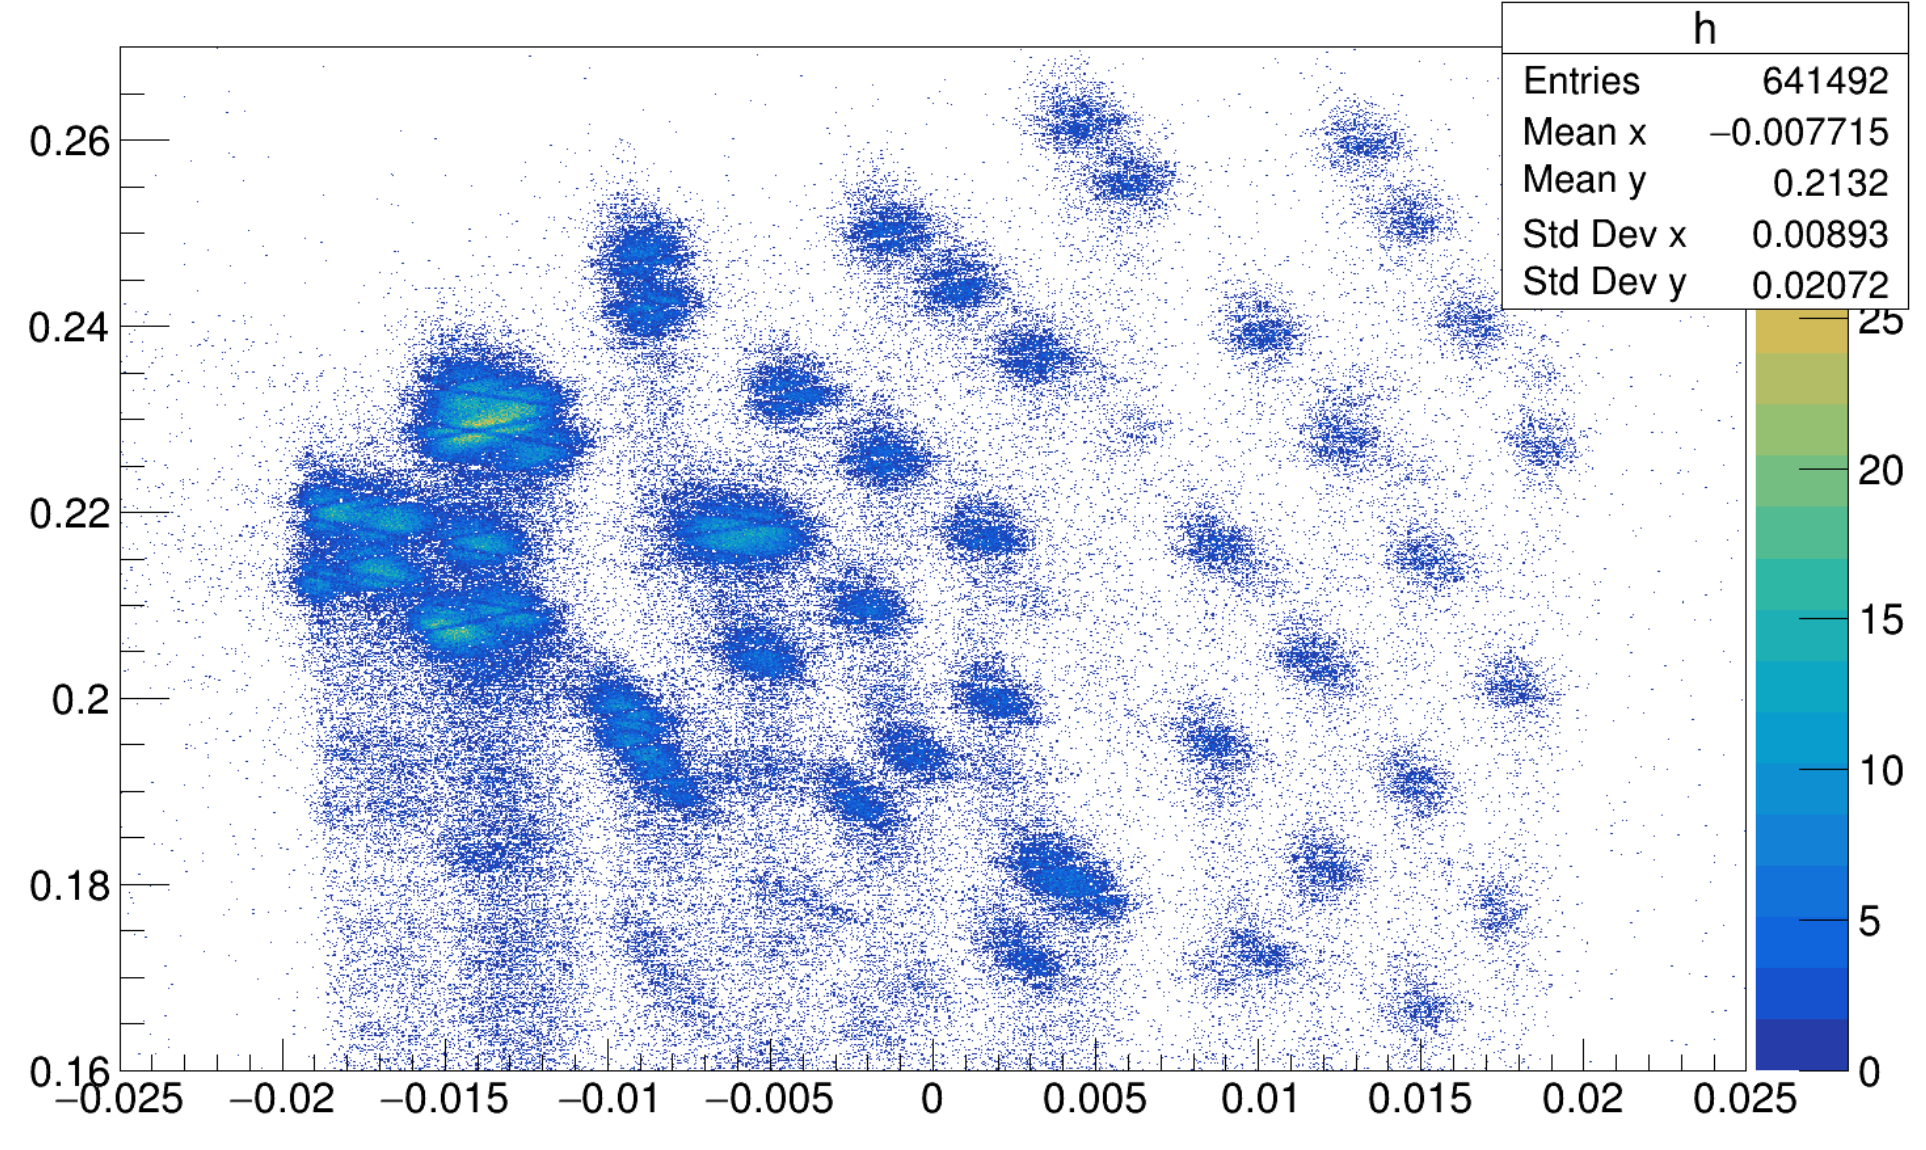
\includegraphics[width=\textwidth]{images/chap4/vdc_t0_before_correction.png}
    \caption{vdc $x$ vs $y$ on vdc detector plane before $T_0$ correction}
    \label{fig:vdc_t0_before_correction}
\end{figure}


\begin{figure}
    \centering
    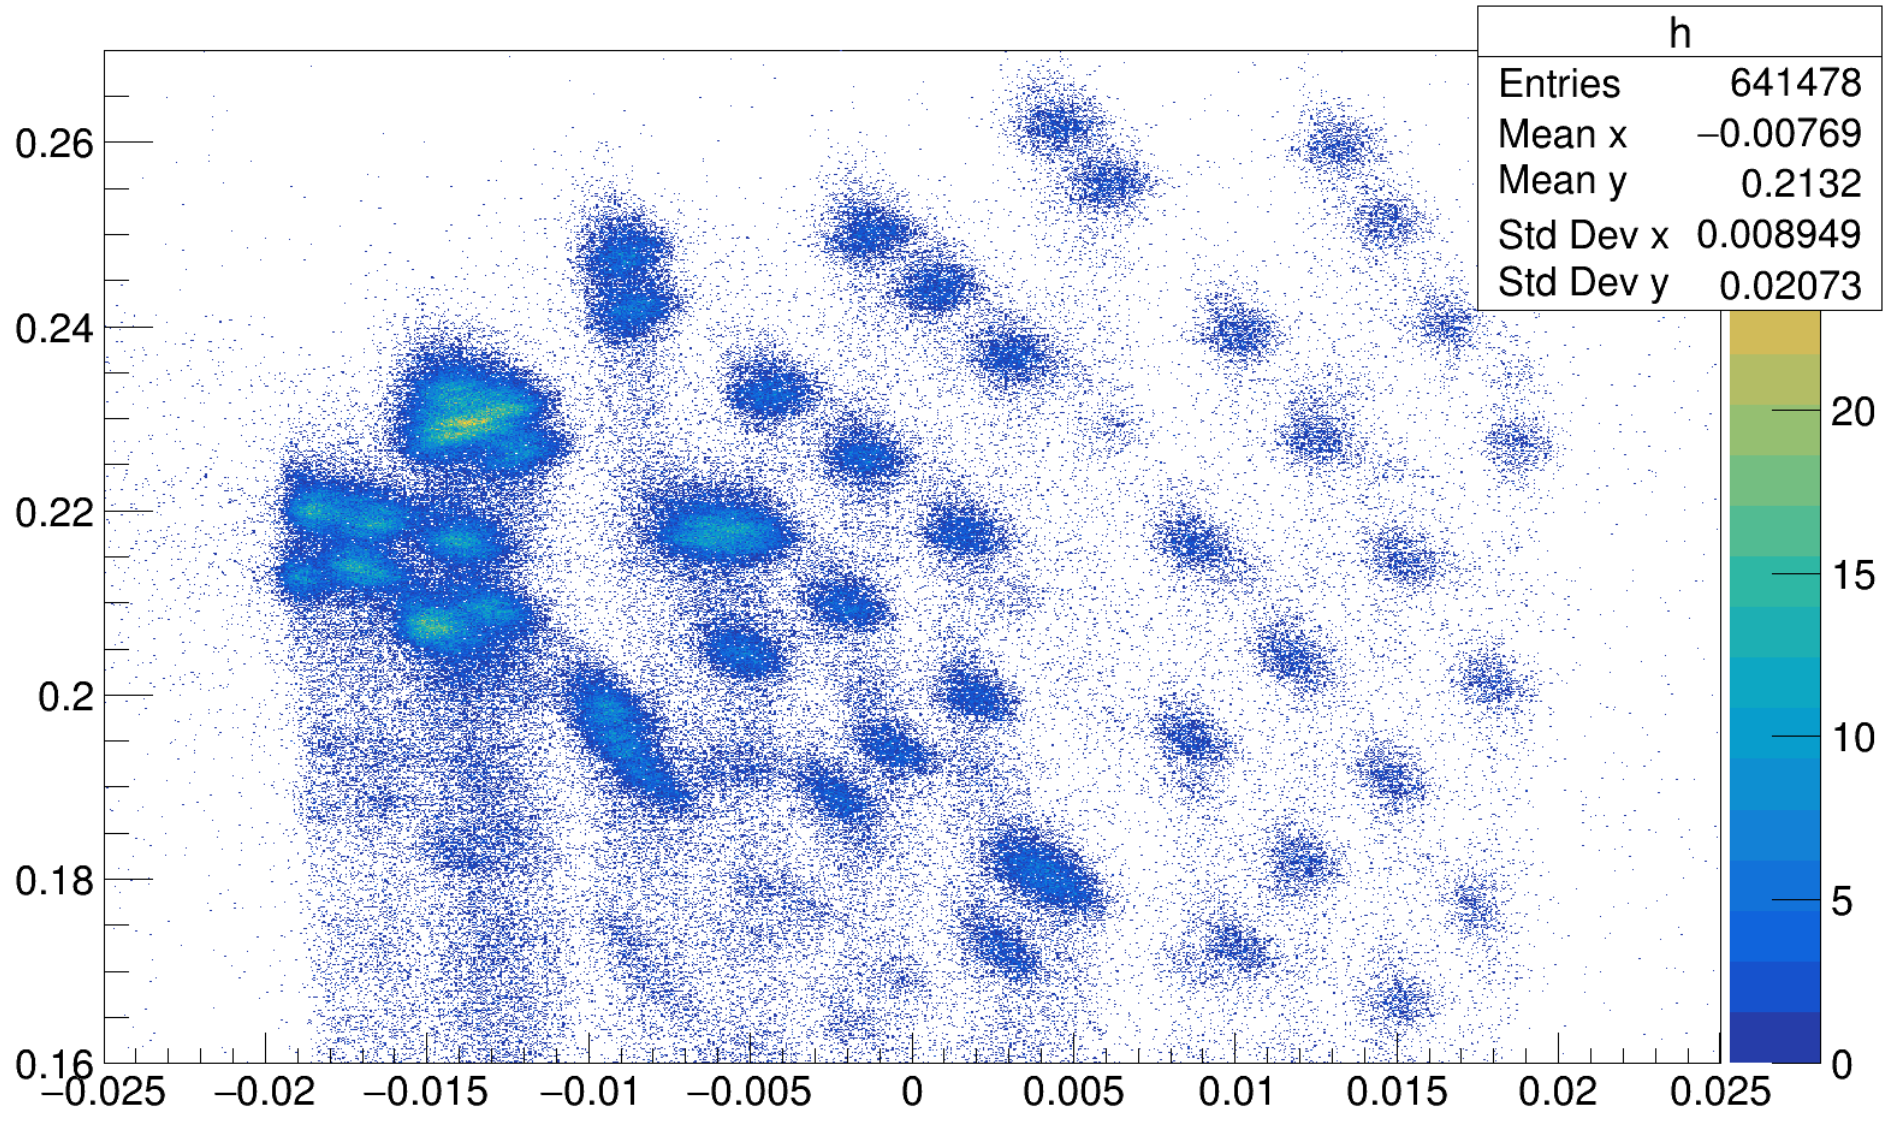
\includegraphics[width=\textwidth]{images/chap4/vdc_t0_after_correction.png}
    \caption{vdc $x$ vs $y$ on vdc detector plane after $T_0$ correction}
    \label{fig:vdc_t0_after_correction}
\end{figure}

The $t_0$ could be calibrated by adjusting the time offset of each TDC channel. In order to calibrate the TDC for all the VDC range, the data should be white spectrum runs that covers all focal plane range with high statistics. 

Here is a procedure of calibration of the TDC $T_0$: [need to check again.]
\begin{enumerate}
    \item Fit the failing tail of the spectrum. 
    \item take the 1.4 $\sigma$ before the peak time
\end{enumerate}

The calibration code can be found in this \hyperlink{https://github.com/Jiansiyu/GeneralScripts/tree/master/VDC_T0_Cali}{GitHub repository}  


\section{High-Resolution Spectrometer Coordinate System}


The Vertical Drift Chamber provides the HRS spatial resolution capability. Each of the two HRS spectrometers contains two Vertical Drift Chamber(VDC). each chamber has 750 wires in two (U, V) planes, position resolution of 100 um per plane. Four VDC chamber layers of wires can provide partial spatial location $x$, $y$ together with particle angle $\theta$ and $\phi$. The kinematics, like scattered angle and scattered momentum, need to derive from the four direct measurable parameters(VDC $x$, $y$,$\theta$,$\phi$). The calibration procedure can be categorized into three steps:

\begin{itemize}
    \item VDC geometry constant calibration 
    \item spatial and angular calibration
    \item momentum calibration
\end{itemize}

Vertical Drift Chamber measures the spatial position by measuring the particle drift time. $t_0$ serves as the starting time of the VDC counter. Carefully calibrated $t_0$ is critical to the spatial and angular resolution of the VDC. To simplify the regression model and easily converge, the spatial, angular, and momentum parameters are calibrated from the focal plane. The VDC geometry constants are used to convert the direct measurements on the VDC plane to the focal plane. Before going into the detail of the calibration, here first introduce the coordination system used in the following contest. 

\subsection{coordinate system}


To simplify the calculation, couples of different coordinate systems are used. In this section, five coordinate systems and their directive relations are briefly introduced. A more detailed coordinate system of Jefferson Lab Hall A can be found in the ESPACE User Manual\cite{espace2002manual}.  

\subsubsection{Hall Coordinate System}
The center of the Hall Coordinate system is defined as the intersection of the electron beam and the vertical symmetry axis of the target system. $z$ is along the beam dump direction. $y$-axis is pointing vertically up against gravity.

[add HCS coordination plot]

\subsubsection{Target Coordinate System}

Each High-Resolution Spectrometer(HRS) has its own target coordinate system. Ideally, the center of the target coordinate system coincides with the center of the Hall A coordinate system. The distance from the hall A center to the midpoint of the center of the sieve slit hole is defined as $Z_0$ ($Z^{HRSE}_0 = 1.181 m$, $Z^{HRSH}_0 = 1.178 m$). The center of the target coordinate system is defined as $Z_0$ distance from the sieve slit(ref to chapter xx section xx) with $z$-axis perpendicular to the center of the sieve slit plane pointing to the beam direction. The $x$-axis is parallel to the sieve slit surface with $x$ pointing vertically down. The $\theta$ and $\phi$ angle is defined as $\frac{dx_{tg}}{Z_0}$ and $\frac{dy_{tg}}{Z_0}$ respectively.

[add TCS plot]


\subsubsection{Detector Coordinate System}

Each of the VDC chambers has 368 wires placed at $\pm 45 ^{\circ} u/v$ direction. The center of the detector coordinate system is defined as the intersection of wire 184 of the VDC1 U1 plane and the perpendicular projection of wire 184 in the VDC1 V1 plane onto the VDC1 U1 plane. $x$-axis is along the long edge of the VDC plane, while y is along the short edge of the VDC plane and $z$ is perpendicular to the VDC plane and pointing upwards. 

Let's take $p_{vdc,n}$ (where ${n=1-4}$)to be the cross position of a particle with each VDC plane. The vertex can be calculated with the following equation. 

\begin{equation}
    \tan \eta_{1} = \frac{p_{vdc,3} - p_{vdc, 1}}{d1}    
\end{equation}
\begin{equation}
    \tan \eta_{2} = \frac{p_{vdc,4} - p_{vdc, 2}}{d1}    
\end{equation}

For ideal experimental configurations, we take the following assumptions:
\begin{enumerate}
    \item All the VDC wires are positioned on a 2D VDC plane
    \item All the VDC wires are oriented in $45\circ$ angle
    \item there is no distortion with the VDC wires
    \item all the VDC frames a perfect parallel to each other 
    \item the center of each VDC plane is known with no error
\end{enumerate}

Given the above assumption, The trajectory position and vertex angles in the detector plane coordinate system can be derived with the following equation 

\begin{equation}
    \theta_{det} = 
\end{equation}
    
\begin{equation}
    \phi_{det} = 
\end{equation}

\begin{equation}
    x_{det} =
\end{equation}

\begin{equation}
    y_{det} =
\end{equation}

Even though the VDC could not be ideal, the distortions would be very small and through HRS Optics, those un-idea errors could be corrected. 

In Hall A analyzer, the VDC result will be given in the detector plane coordinate system.

[add vdc, DCS plot]

\subsubsection{Transport Rotation Coordinate System at the focal plane}
The transport coordinate system at the focal plane is defined as rotating the detector coordinate system by $45^{\circ}$ along the y-axis. Ideally the z-axis along the central beam ray. 

Given the particle position at the detector coordinate system, the transport rotation coordinate system can be derived as:

\begin{equation}
    \theta_{tra}  = 
\end{equation}

\begin{equation}
    \phi_{tra} =
\end{equation}

\begin{equation}
    x_{tra} =
\end{equation}

\begin{equation}
    y_{tra} = 
\end{equation}


[add the plot of the transport coordinate system plot]


\subsubsection{Focal plane Coordinate System}

The focal plane coordinate system used for HRS analysis is a rotated coordinate system, obtained by rotating the Detector Coordinate System (DCS) around its y-axis by an angle. This angle is determined by the angle between the local central ray and the z-axis of the DCS, and as a result, the z-axis of the Focal Plane Coordinate System (FCS) rotates as a function of the relative momentum p. Because of the focusing of HRS magnet system,  particle from different scattering angles with same momentum will be focused at the focal plane. therefore, the relative momentum to the central momentum of the spectrometer which defined as 
\begin{equation}
    \delta = \frac{p-p_0}{p_0}
\end{equation}

this factor approximately only depends on $x_{tra}$ and $p_0$.

To ensure easy convergence, the HRS Optics Tensor is calibrated with respect to the angles $\theta$ and $\phi$, the vertical position $y$, and the relative momentum $dp$ on the Focal Plane Coordinate System.

\begin{equation}
    x_fp = x_{tra}    \label{eq:cpt3_fps_1}
\end{equation}

\begin{equation}
    y_{fp} = y_{tra} - \sum y_{i000}x^i_{fp}  
\end{equation}

\begin{equation}
\theta_{fp} = \frac{\theta_{det} + \tan\rho}{1 - \theta_{det}\tan\rho}
\end{equation}


\begin{equation}
    \phi_{fp} = \frac{\phi_{det} - \sum p_{i000}x^i_{fp}}{cos \rho - \theta_{det} sin\rho}
\end{equation}

here  in the equation:

\begin{equation}
    \tan\rho  = \sum t_{i000}x^i_{fp} \label{eq:cpt3_fps_5}
\end{equation}


the code used for calibration of the focal plane constant can be found on this GitHub repository: \hyperlink{https://github.com/Jiansiyu/GeneralScripts/blob/master/vdcConstantOpt}{GitHub Repository Link}


[need to add the Focal plane coordination system plot]

\section{focal plane constant calibration}

The HRS Spectrometer Focal Plane Coordinate System is a rotated system, with the Z-axis being the projection of the local central ray on the x-z plane. The origin of this coordinate system is shared with the detector coordinate system. To correct the coordinate system, we use a criterion based on the ideal case of the central beam passing through the central sieve hole, where the beam position is (0,0). Specifically, we look at the equation of the focal plane coordinate system, where a parameter is used to project the coordinate system. To achieve high accuracy, each parameter is optimized to the 3rd order.

In the Hall A analyzer, the correction constant can be found in the first three rows of the x.vdc.matrixelem variable:

\begin{center}
    \captionof{focal plane correction constant}
    \begin{tabular}{c c c c c c c c}
        t & 0 & 0 & 0 & -1.001135e+00 & -3.313373e-01 & -4.290819e-02 & 4.470852e-03 \\
        y & 0 & 0 & 0 & -8.060915e-03 & 1.071977e-03 & 9.019102e-04 & -3.239615e-04 \\
        p & 0 & 0 & 0 & -2.861912e-03 & -2.469069e-03 & 8.427172e-03 & 2.274635e-03
    \end{tabular}
    
\end{center}

Here, the first column indicates the parameter name, followed by the orders of $\theta$, $\phi$, and $dp$ (all 0s in this case), and the constant factors of $x^0$, $x^1$, $x^2$, $x^3$.

According to the focal plane coordinate system definition, for the central beam passing through the central sieve hole, we have $\theta_{focal}=0$, $\phi_{focal}=0$, and $y_{focal}=0$.

To optimize the correction constant, we follow these steps:

\begin{enumerate}
    \item Gather as many runs as possible at any central P runs.
    \item Select the events that pass through the central sieve hole.
    \item Calculate the detector plane parameters for all the events.
    \item Define the loss function as the square residual of the focal plane calculated using the detector coordinate variables (given by equations \ref{eq:cpt3_fps_1} to \ref{eq:cpt3_fps_5}) and the theoretical value of 0.
    \item Optimize the loss using a linear regression model, and obtain the constants $t_{i000}$, $y_{i000}$, and $p_{i000}$.
\end{enumerate}


\begin{figure}
    \centering
    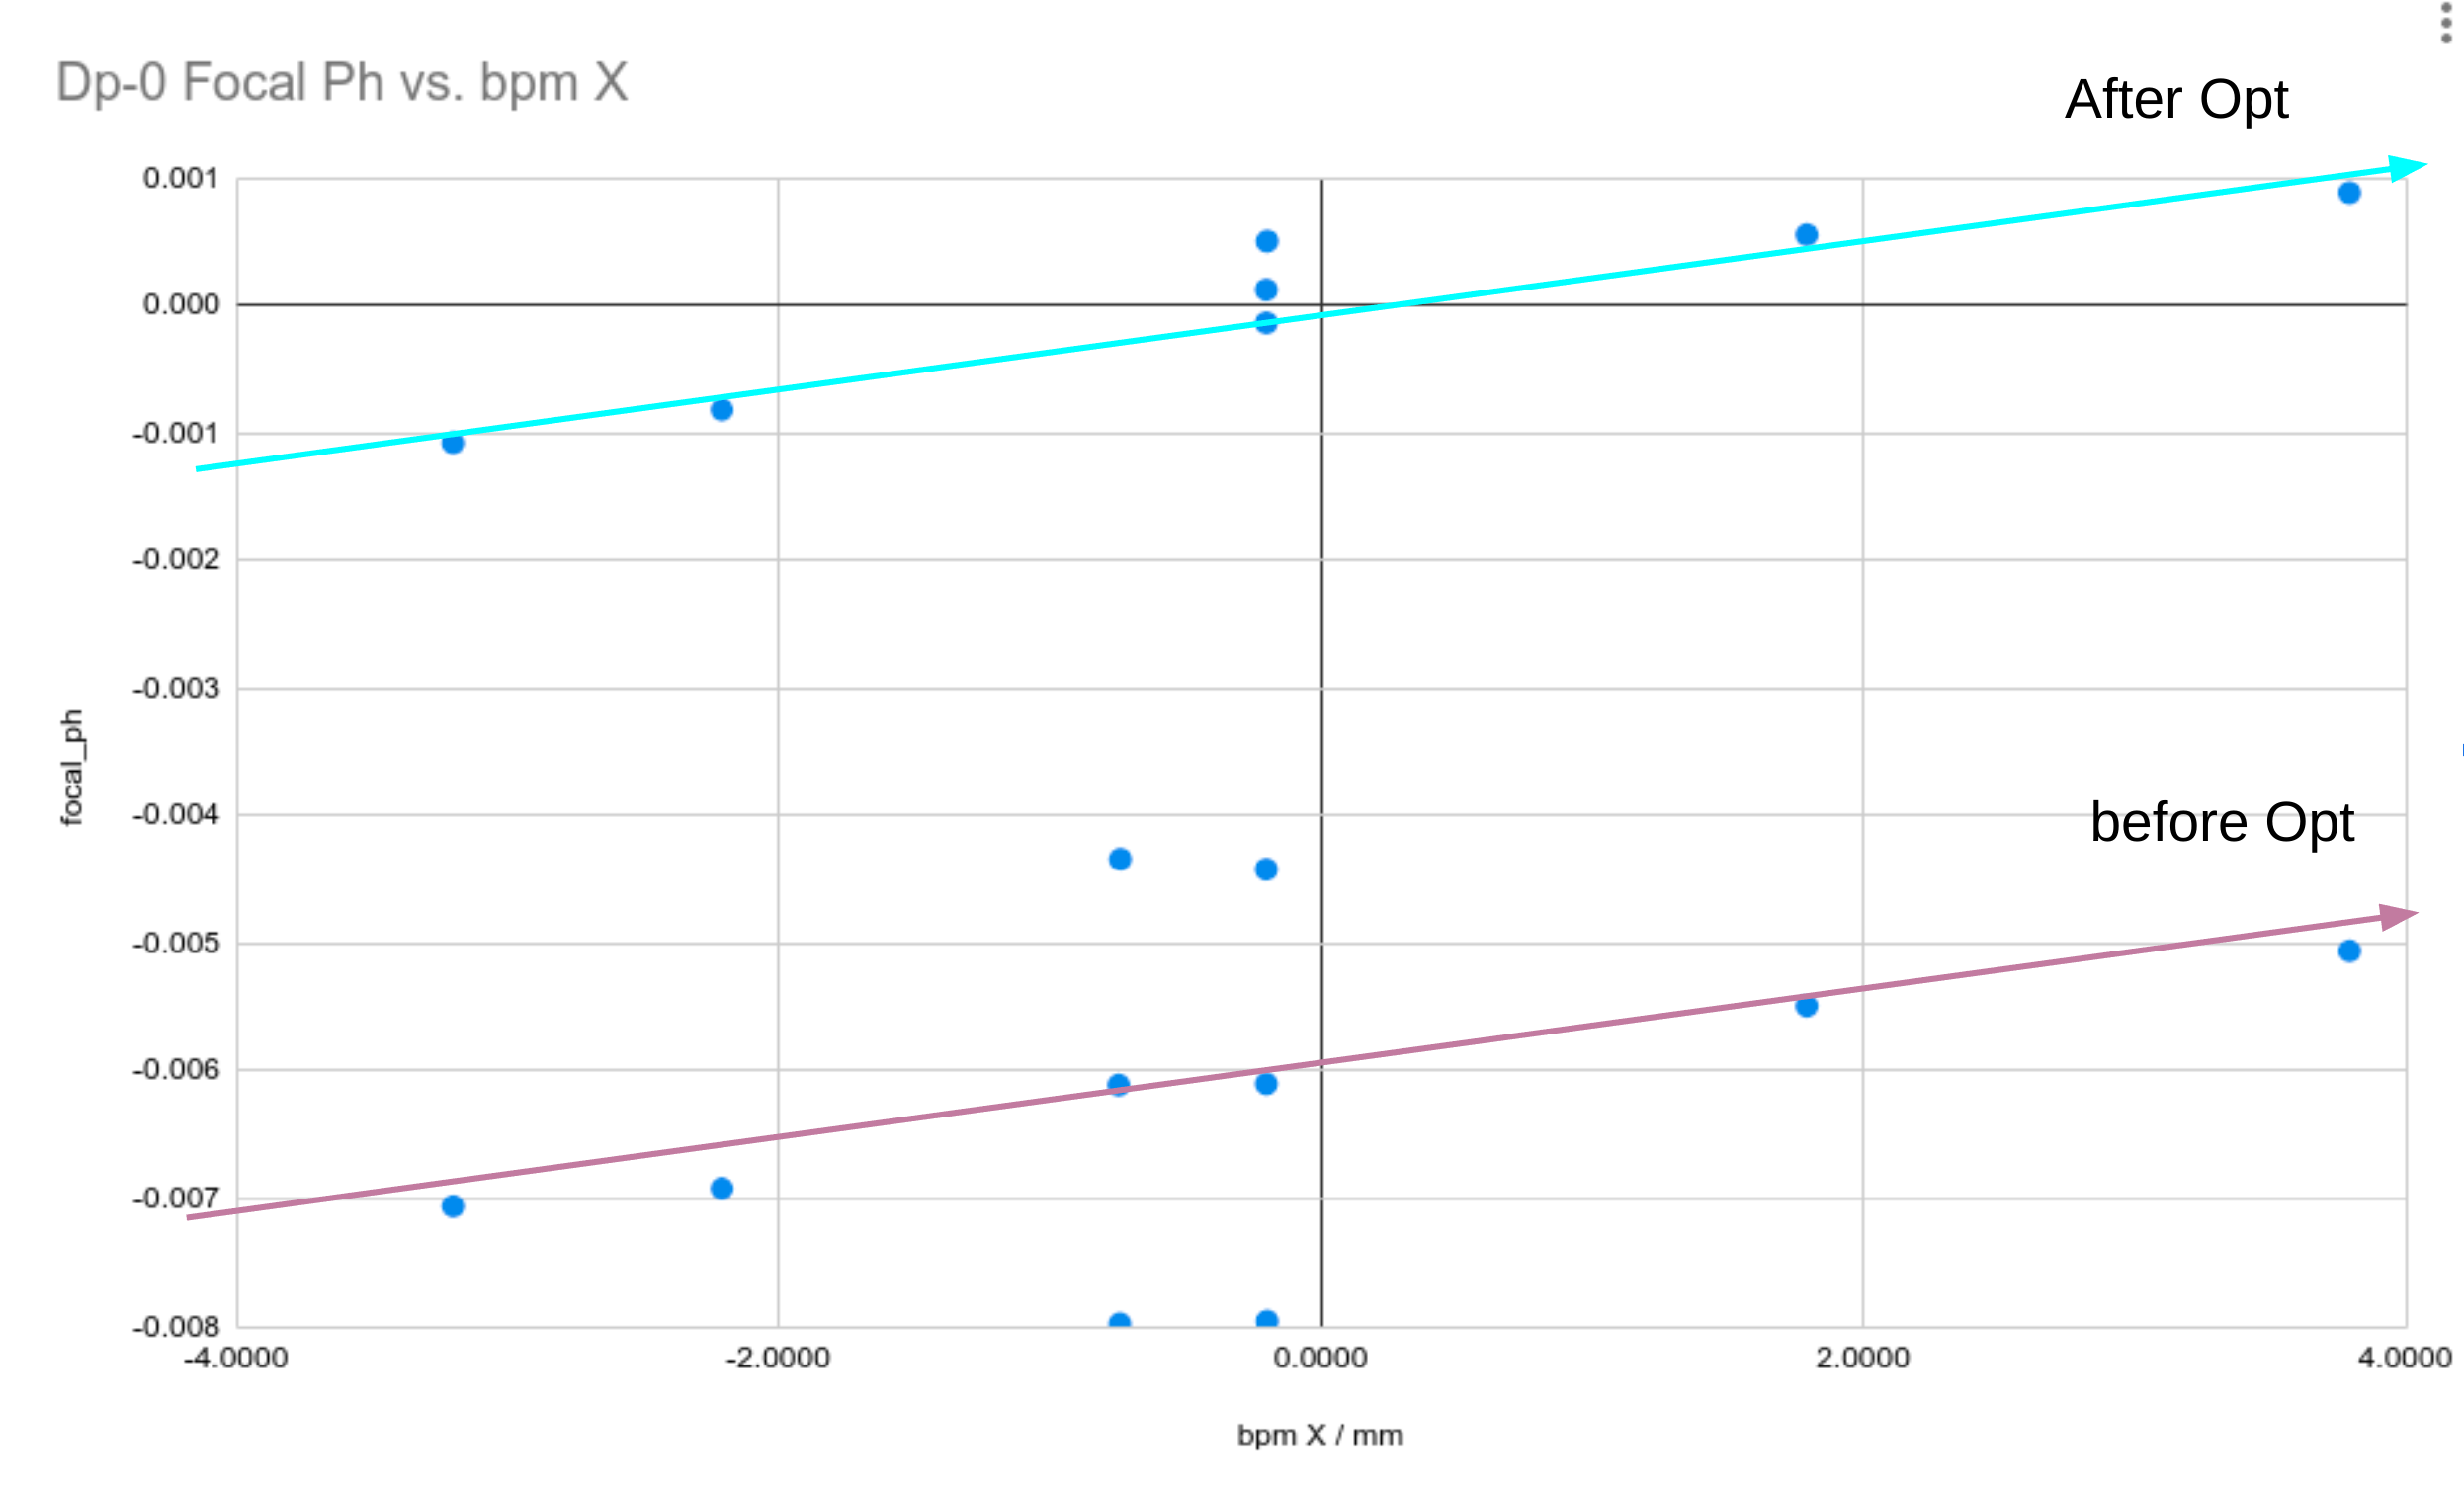
\includegraphics[width =\textwidth]{images/chap4/vdcconstant_focal_bpmx.png}
    \caption{$\phi_{focal}$ vs. $x_{bpm}$ before and after focal plane constant correction [to be replaced]}
    \label{fig:focal_ph_bpm_x_constant_correction_plt}
\end{figure}


\begin{figure}
    \centering
    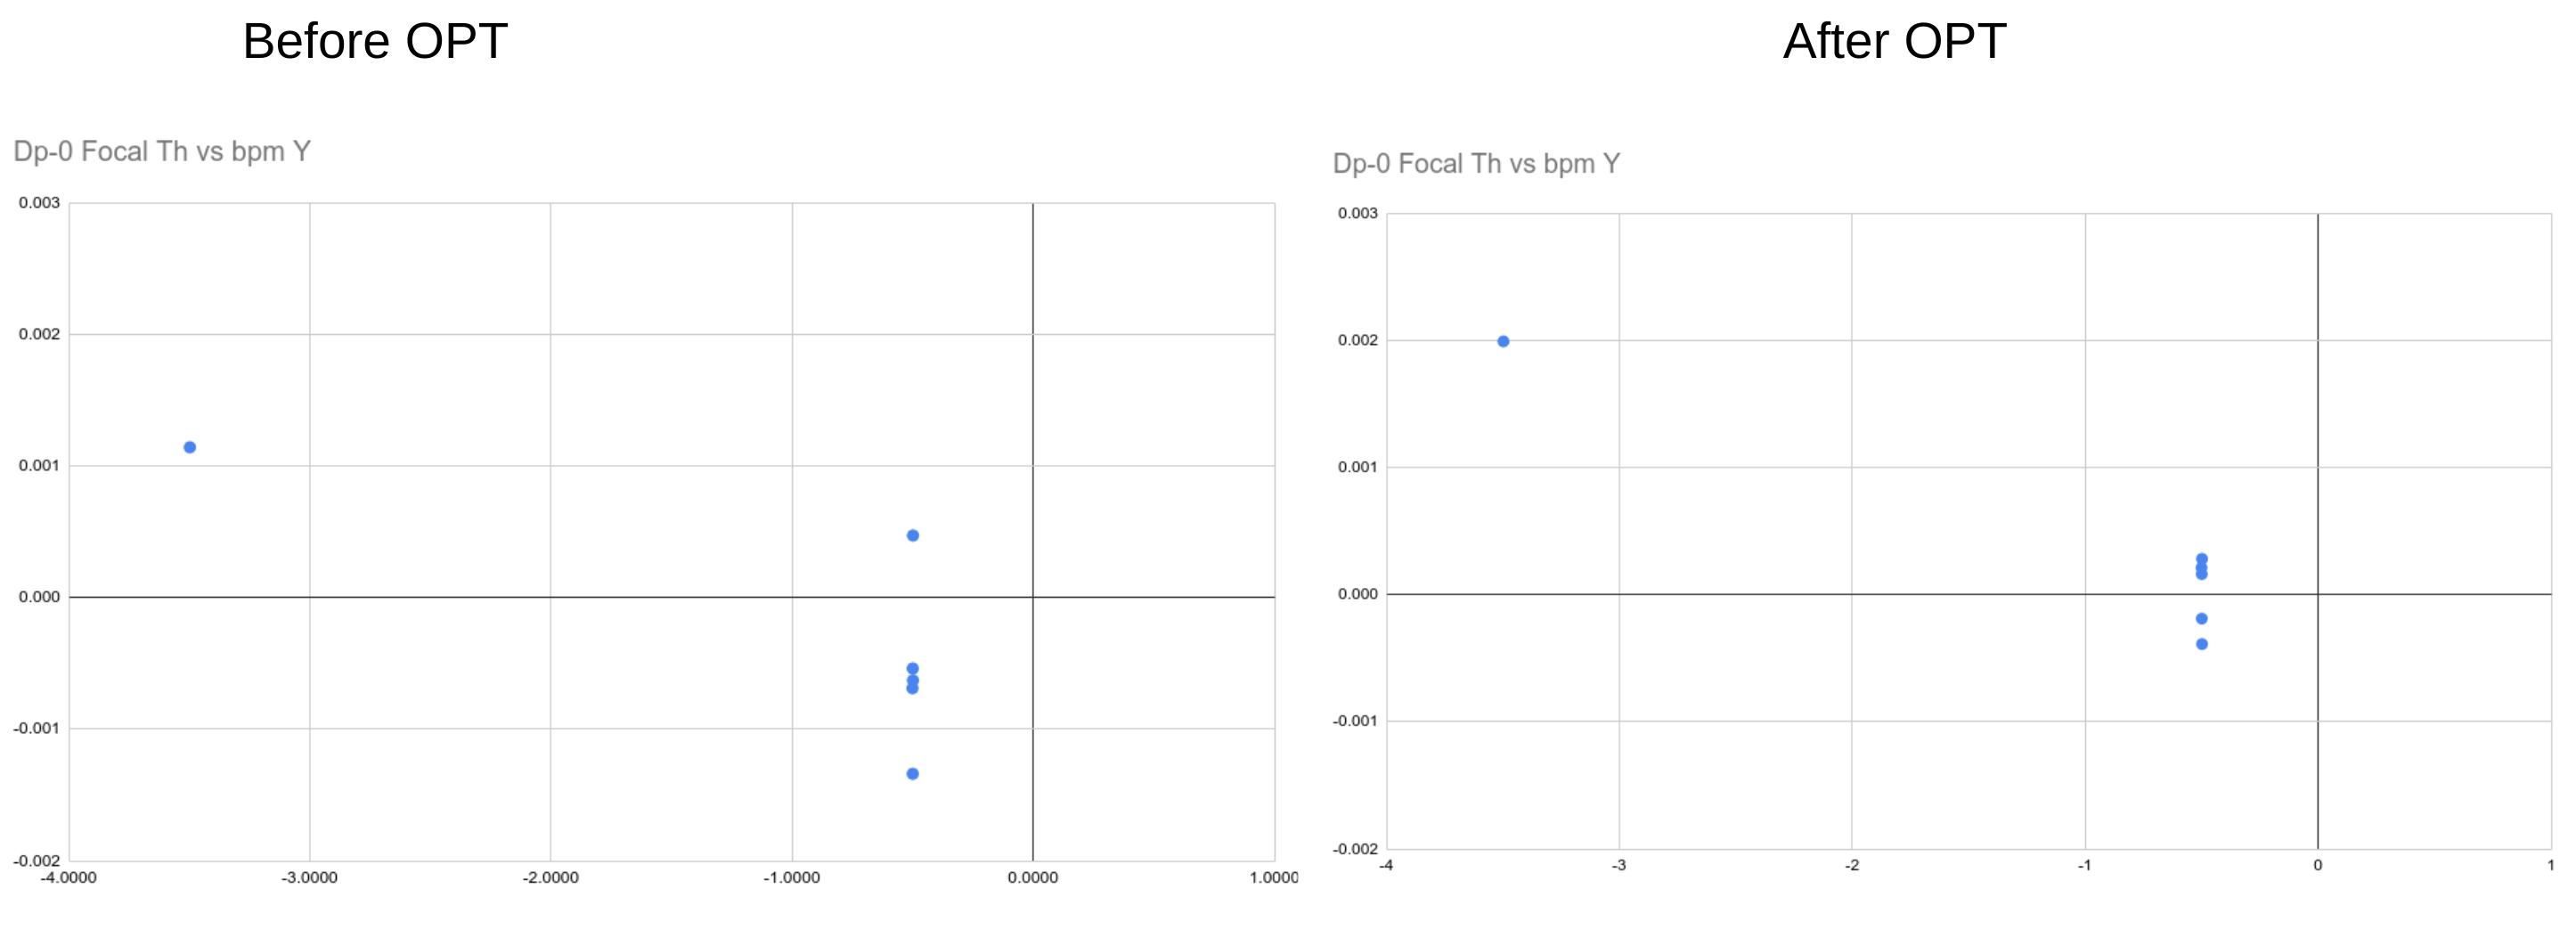
\includegraphics[width =\textwidth]{images/chap4/vdcconstant_focal_th_bpmy.png}
    \caption{$\theta_{focal}$ vs. $y_{bpm}$ before and after focal plane constant correction [to be replaced]}
    \label{fig:my_label}
\end{figure}

\begin{figure}
    \centering
    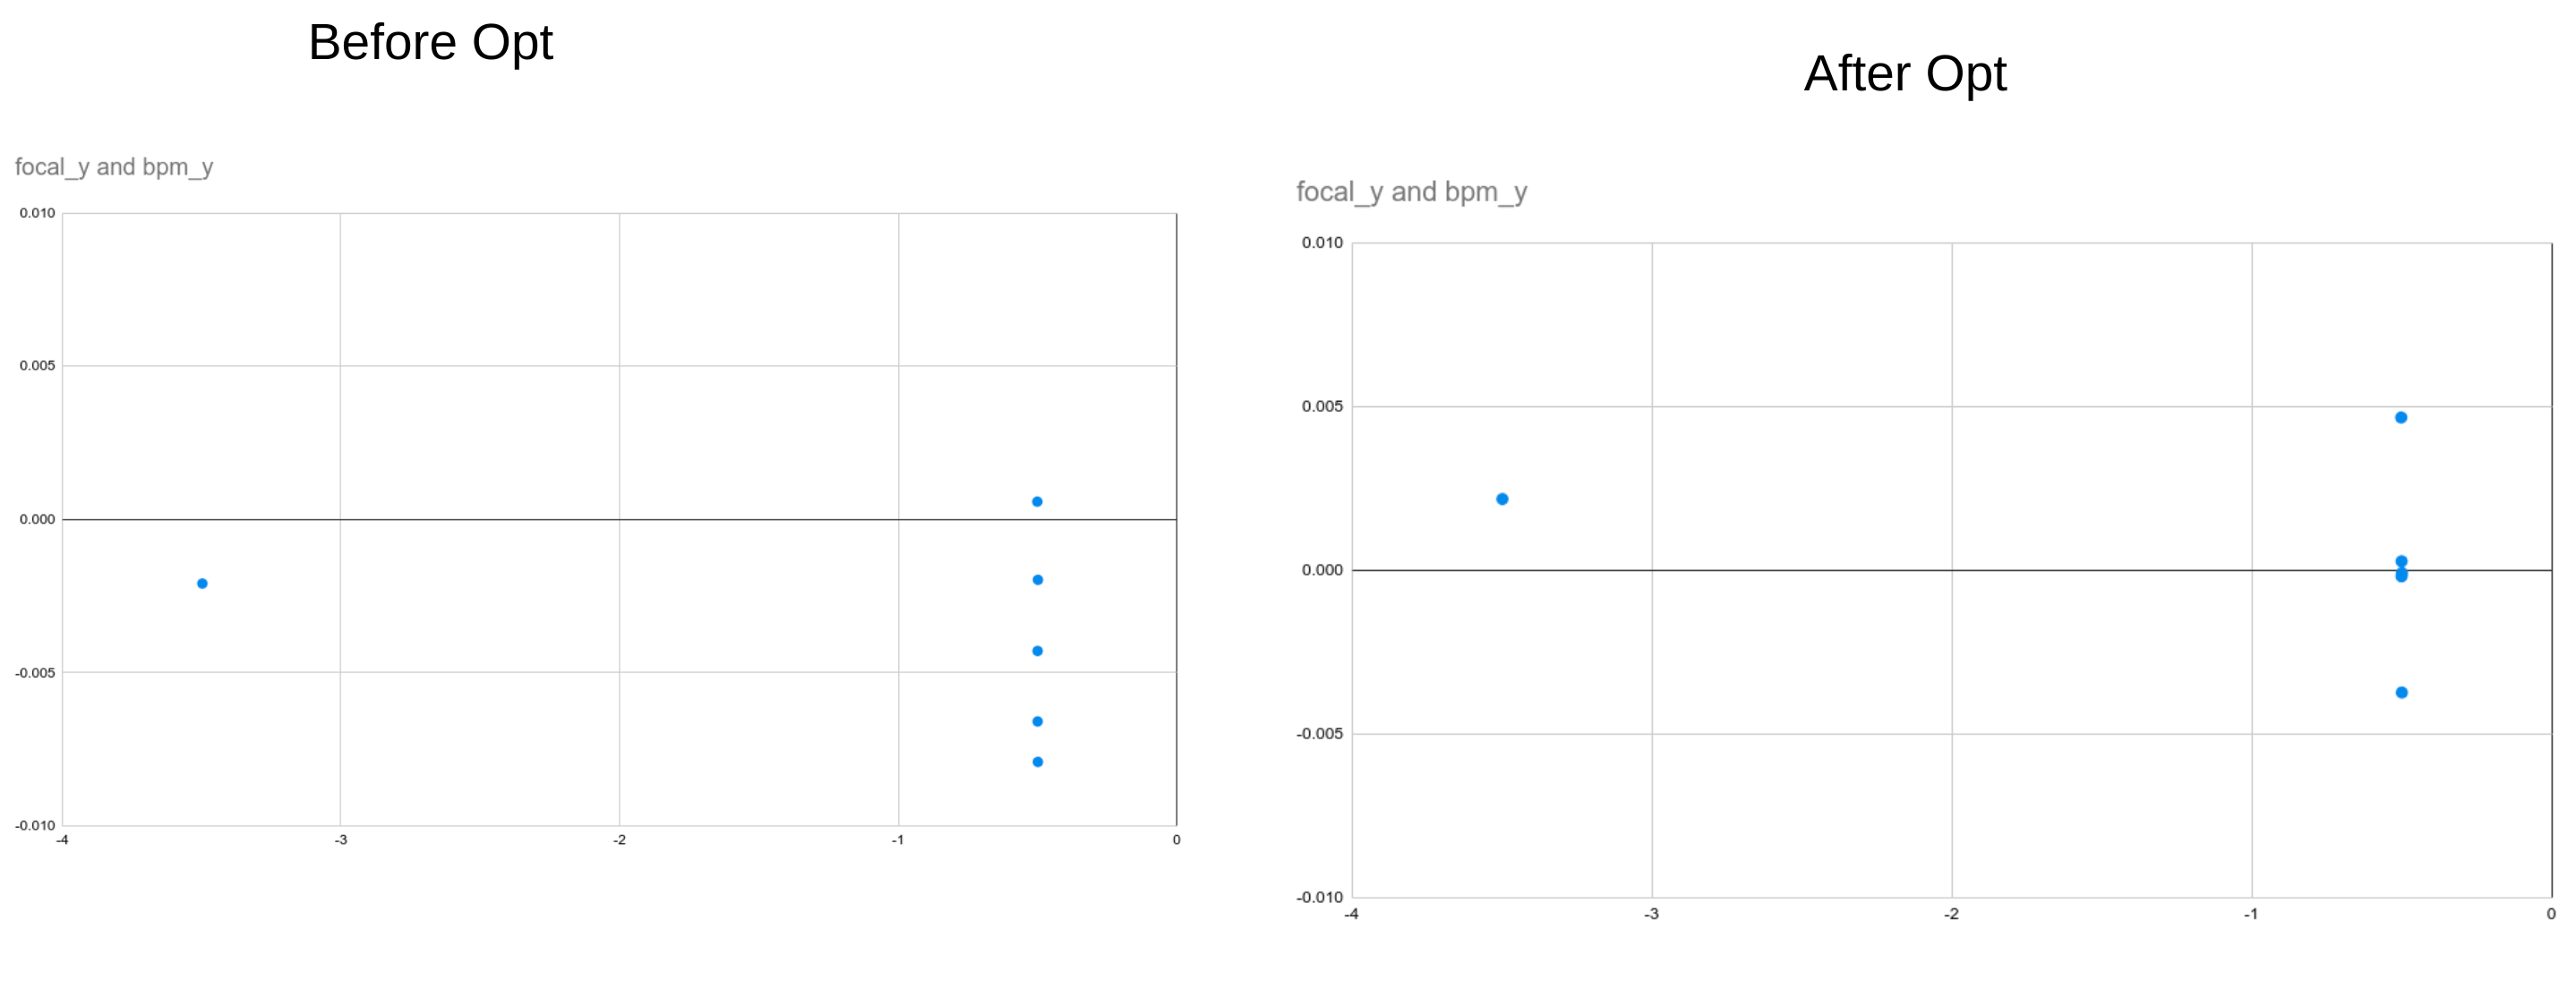
\includegraphics[width =\textwidth]{images/chap4/vdcconstant_focaly_bpmy.png}
    \caption{$y_{focal}$ vs. $x_{bpm}$ before and after focal plane constant correction [to be replaced]}
    \label{fig:my_label}
\end{figure}

From the plot we could see, after the optimization, with the new constant $t_{i000}$,$y_{i000}$,$p_{i000}$, the central sieve $\theta_{focal}$,$\phi_{focal}$,$y_{focal}$ are set to $(0,0,0)$.


\section{High-Resolution Spectrometer Calibration}

In the preceding section, we introduced the calibration process used to map the detector coordinate system onto the focal plane coordinate system. In this section, we will delve into HRS Optics, specifically focusing on the transformation from the focal plane coordinate system to the target coordinate system.

\subsection{Approach}

With the previous introduction, the direct measurement the position on the 4 vertical drift chambers $p_{vdc,i}$ together with the displacement of the chambers $d$ are converted to the focal plane coordinate system, $x_{fp}$,$y_{fp}$,$\theta_{fp}$,$\phi_{fp}$. Those observables are used to calculate $\theta_{tg}$,$\phi_{tg}$,$y_{tg}$, and $\delta_{tg}$ on the target which we used for further physics analysis. 

The conversion from the focal plane coordinate system to the target coordinate system is with the transport tensors. In first-order approximation, the relation between the two coordinate systems can be written as:

\begin{equation}
\begin{bmatrix}
\delta_{tg} \\
\theta_{tg} \\
y_{tg} \\
\phi_{tg}
\end{bmatrix} = \begin{bmatrix}
    <x_{fp}|x_{fp}> & <x_{fp}|\theta_{fp}> & 0 & 0 \\
    <\theta_{fp}|x_{fp}> & <\theta_{fp}|\theta_{fp}> & 0 & 0 \\
    0 & 0 & <y_{fp}|y_{fp}> & <y_{fp}|\phi_{fp}>  \\
    0 & 0 & <\phi_{fp}|y_{fp}> & <\phi_{fp}|\phi_{fp}>  
\end{bmatrix} * \begin{bmatrix}
    x_{fp} \\
    \theta_{fp} \\
    y_{fp} \\
    \phi_{fp}
\end{bmatrix}
\end{equation}

Because of the mid-plane symmetry of the spectrometer, 8 of the reverse corner element are $0$.'

% explain why it is to $$x^n$$ order? what is the physics meaning of 

In practice, the expansion of the focal plane coordinates is performed up to the fifth order and use the polynomial production of the four observables as features in modeling the spectrum. 

\begin{equation}
    y_{tg} = \sum_{jkl}Y_{jkl}\theta^j_{fp}y^k_{fp}\phi^l_{fp}
\end{equation}


\begin{equation}
    \theta_{tg} = \sum_{jkl}T_{jkl}\theta^j_{fp}y^k_{fp}\phi^l_{fp}
\end{equation}


\begin{equation}
    \phi_{tg} = \sum_{jkl}P_{jkl}\theta^j_{fp}y^k_{fp}\phi^l_{fp}
\end{equation}


\begin{equation}
    \delta_{tg} = \sum_{jkl}D_{jkl}\theta^j_{fp}y^k_{fp}\phi^l_{fp}
\end{equation}

Where in the above equations, tensors $Y_{jkl}$, $T_{jkl}$, $P_{jkl}$, $D_{jkl}$ are are polynomial of $x_fp$ for example, $Y_{ijk}$ can be write as:

\begin{equation}
    Y_{jkl} = \sum^m_{i=1}C_i^{Y_{jkl}}x^i_{fp}
\end{equation}

In the equation, $C^i_{jkl}$ is the $x^i$ correction constant for $Y_{jkl}$. The final equation can be written as:

\begin{equation}
    y_{tg} = \sum_{jkl} (\sum^m_{i=1}C_i^{Y_{jkl}}x^i_{fp}) \theta^j_{fp}y^k_{fp}\phi^l_{fp}
\end{equation}


\begin{equation}
    \theta_{tg} = \sum_{jkl}(\sum^m_{i=1}C_i^{T_{jkl}}x^i_{fp})\theta^j_{fp}y^k_{fp}\phi^l_{fp}
\end{equation}


\begin{equation}
    \phi_{tg} = \sum_{jkl}(\sum^m_{i=1}P_i^{Y_{jkl}}x^i_{fp})\theta^j_{fp}y^k_{fp}\phi^l_{fp}
\end{equation}


\begin{equation}
    \delta_{tg} = \sum_{jkl}(\sum^m_{i=1}D_i^{Y_{jkl}}x^i_{fp})\theta^j_{fp}y^k_{fp}\phi^l_{fp}
\end{equation}

Here is an example of Y in the vertical drift chamber database:

\begin{center}
    % \captionof{focal plane correction constant}
    \begin{tabular}{c c c c c c c }
        D& 0& 0& 0&  8.851691E-04& 7.570314E-02& 1.116963E-02\\
        D& 0& 0& 1&  4.667677E-02& 9.485094E-02&
    \end{tabular}    
\end{center}

In the first row, $D$ indicates this is the tensor for the $\delta_{tg}$, the following three integers is corresponding to the power of $\theta$,$y$,$\phi$, which is $jkl$ in the equation. The following float number is the $i=1$ constant, $i=2$ constant and etc. 


To achieve high optics accuracy, each element is optimized up to the fifth order. Because of the overfitting issue if there are too many features present in the model, in the optimization practice, not all the orders are kept for each tensor. In the training process, each feature is carefully tested to make sure it will not cause serious overfitting and get the best test result on the holdout dataset. 

[add how to select the features that most suitable for the model??]

\subsection{Ground Truth data set}

In order to construct a precise regression model for the HRS spectrometer, a highly accurate ground truth dataset is essential. This ground truth is derived from a meticulously crafted CNC-made sieve plate. It is a stainless steel plane with holes in the grid. Every hole is manufactured with a high accurate cnc machine. With the given position of each sieve hole, we can calculate the theoretical value for the scattering angle as well as the momentum for each sieve hole. Those sieve holes provide us with an accurate calibration point for the HRS. 

The sieve plate is strategically positioned in front of the septum magnet, with its location carefully surveyed to ensure a positional accuracy of up to 100 micrometers. As electrons scatter from the target, only those that pass through the holes on the sieve plate are allowed to enter the spectrometer and ultimately reach the vertical drift chamber. All other electrons are effectively blocked by the sieve plate.

Upon reaching the vertical drift chamber, particles that have passed through the same hole on the sieve plate will form a distinct cluster. By categorizing events based on these clusters and considering the relative positions of the clusters on the sieve plate, it is possible to determine which holes the particles have originated from. With this information, the ground truth values can be calculated for each sieve hole.

In the following sections, we will delve into the details of calculating the ground truth values used to calibrate the HRS spectrometer, ensuring the highest level of accuracy and precision in the model.

\subsubsection{apparatus [need to rewrite]}

\begin{figure}
    \centering
    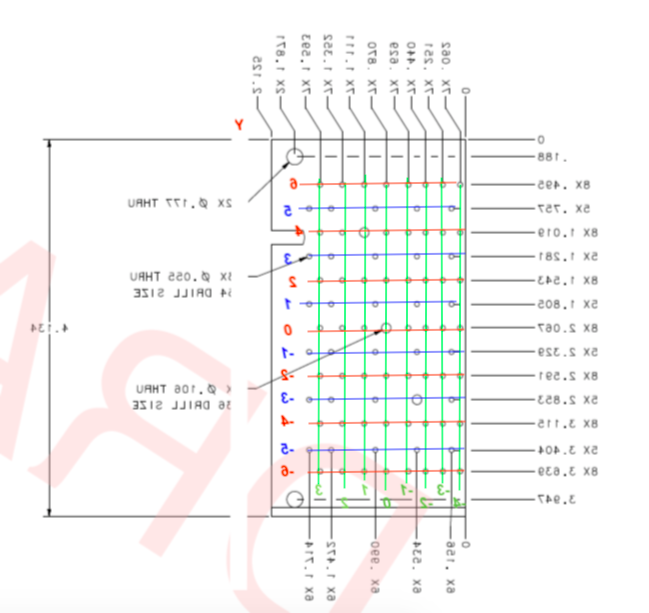
\includegraphics[width =\textwidth]{images/chap4/sieve_cnc_draw.png}
    \caption{PRex-II sieve slit used for Optics Calibration, three big holes are used for identifying the orientation of the reconstructed data}
    \label{fig:sieve_cnc_draw}
\end{figure}


\begin{figure}
    \centering
    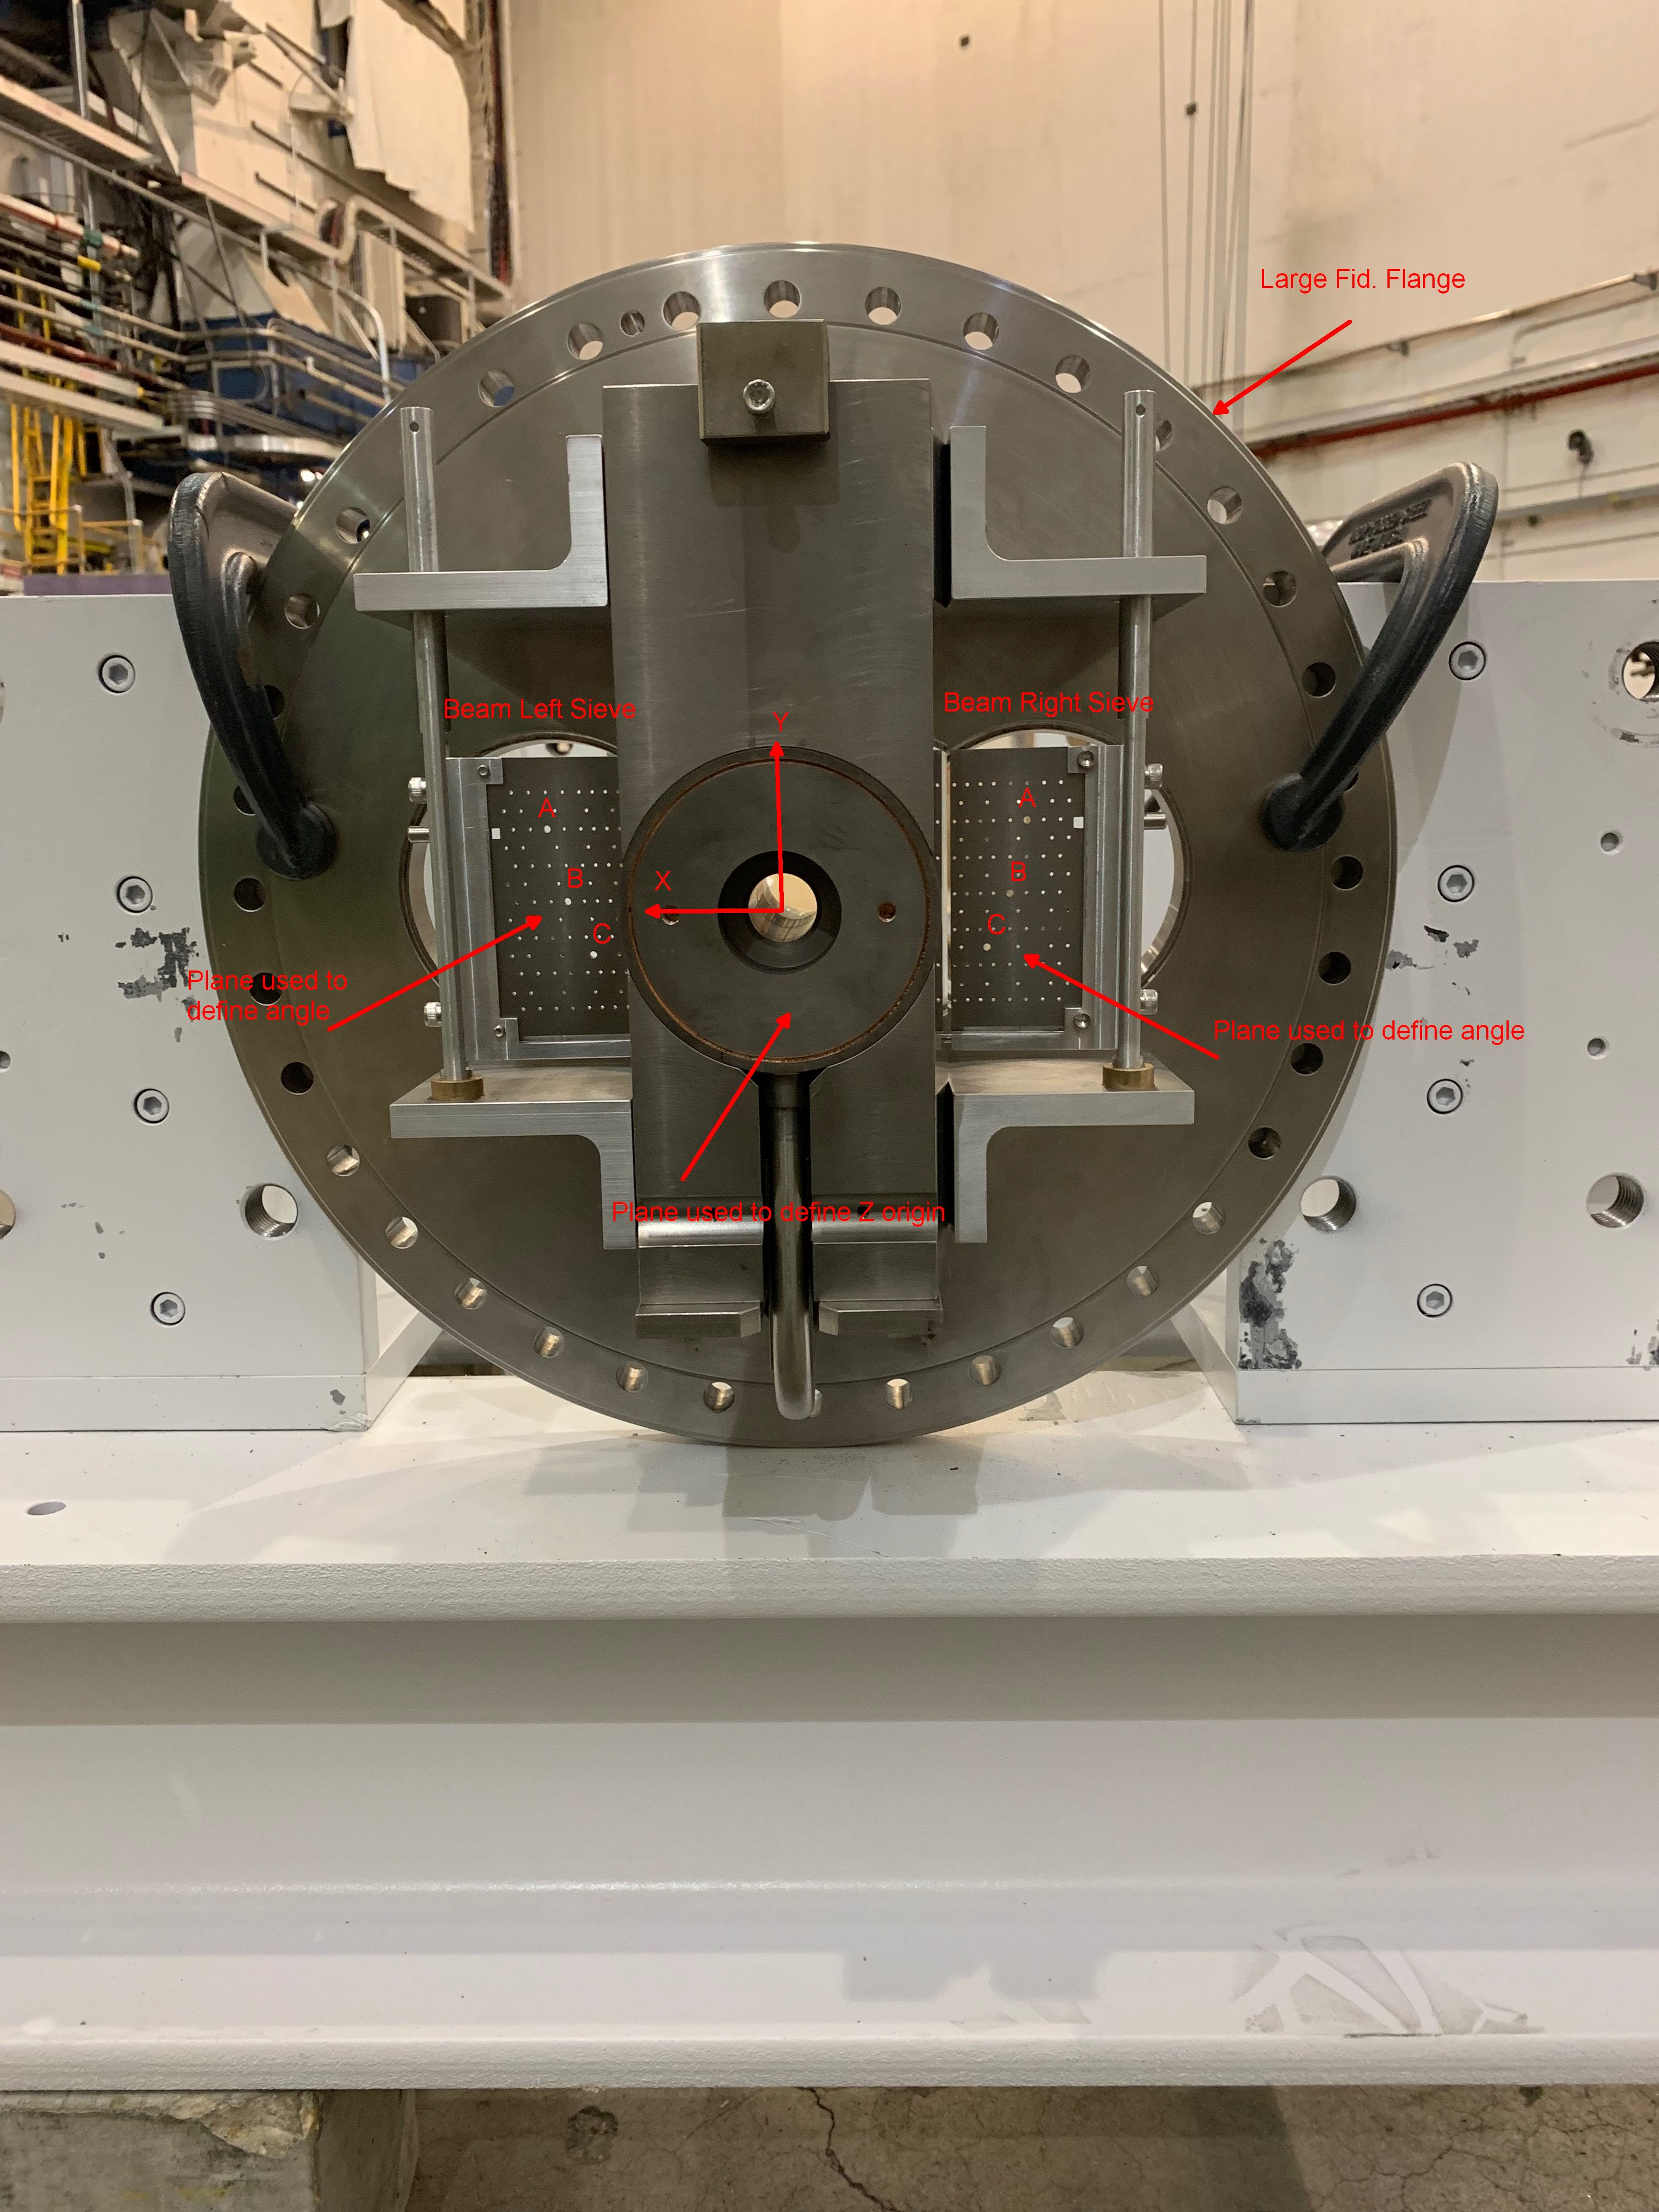
\includegraphics[width =\textwidth]{images/chap4/sieve_in_hrs.jpg}
    \caption{PRex-II/CRex Sieve slit in the High-resolution spectrometer}
    \label{fig:labeled_sieve_in_hrs}
\end{figure}


\begin{figure}
    \centering
    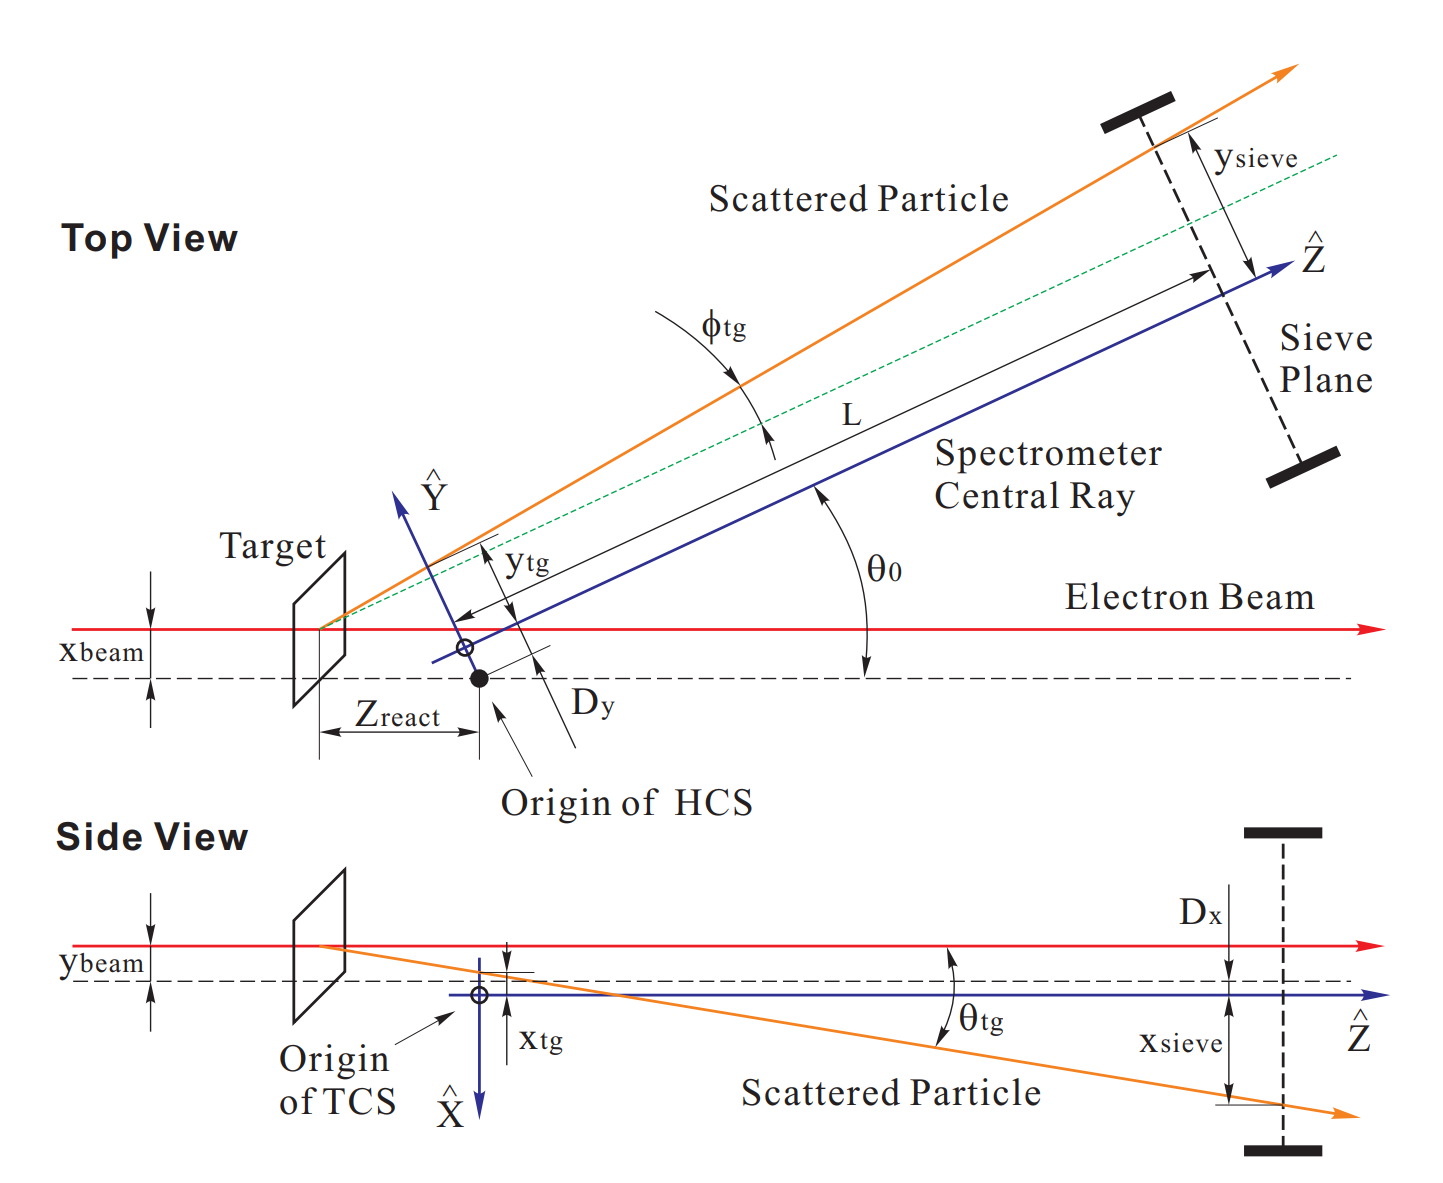
\includegraphics[width =\textwidth]{images/chap4/target_coordinate_system.png}
    \caption{Target Coordinate System}
    \label{fig:target_coordinate_system_plot}
\end{figure}

Figure \ref{fig:sieve_cnc_draw} displays the schematic of the sieve plate. The Hall A survey is conducted in the Hall A coordinate system and measured relative to the center of the sieve plate. In the target coordinate system, the origins of both the target and hall coordinate systems are assumed to be identical. However, in practice, the center of the target coordinate system deviates from that of the hall coordinate system. These deviations in the horizontal and vertical directions are denoted by $D_y$ and $D_x$, respectively. The ground truth result in the target coordinate system can be computed using the following equations:

\begin{equation}
\phi_{tg} = \frac{y_{sieve} + D_y - x_{beam}\cos{\theta_0} + z_{react}\sin{\theta_0}}{L - z_{react}\cos{\theta_0 - x_{beam}\sin{\theta_0}}}
\end{equation}

\begin{equation}
\theta_{tg} = \frac{x_{sieve} + D_x + y_{beam}}{L - z_{react}\cos{\theta_0} - x_{beam}\sin{\theta_0}}
\end{equation}

\begin{equation}
y_{tg} = y_{sieve} - L \phi_{tg}
\end{equation}

\begin{equation}
x_{tg} = x_{sieve} - L \theta_{tg}
\end{equation}

Where in the equation $\theta_0$ is the spectrometer central angle measured by the angle of the beam down direction and the central sieve hole. $L$ is the distance from the target location to the central sieve slit hole. Using these equations, the scattered angle and reaction point can be determined with the help of the beam variables measured in the hall coordinate system, as given by:

\begin{equation}
\theta_{scatter} = \arccos\left(\frac{\cos{\theta_0} - \phi_{tg}\sin{\theta_0}}{\sqrt{1 + \theta^2_{tg} + \phi^2_{tg}}}\right)
\end{equation}

\begin{equation}
z_{react} = \frac{-(z_{tg} + D_y) + x_{beam}(\cos{\theta_0} - \phi_{tg}\sin{\theta_0})}{\cos{(\theta_0\phi_{tg} + \sin{\theta_0})}}
\end{equation}

For the PRex-II experiment, only one target foil was employed. As a result, $z_{react}$ and $x_{react}$ are both 0. The constant spectrometer length $L$ and the central sieve angle in the Hall Coordinate System (HCS) are calculated using the survey results. For PRex-II experiment, the equations can be rewritten as:

\begin{equation}
    \theta_{tg} = \arctan{\frac{x_{sieve}}{L}}
\end{equation}

\begin{equation}
    \phi_{tg} = \arctan{\frac{y_{sieve} - x_{beam}\cos{\theta_0} + D}{L - x_{beam}\sin{\theta_0}}}
\end{equation}

\begin{equation}
    y_{tg} = y_{sieve} - L \frac{y_{sieve}-x_{sieve}\cos{\theta_0} + D}{L - x_{sieve}\sin{\theta_0}}
\end{equation}

After getting the ground truth values, with the help of the spectrometer tensor, we can project the measurement from the focal plane coordinate system to the target system, which is considered to be the predicted value in the optimization procedure. The loss function takes L2 loss, which is the square error between the predicted value and the ground truth. 


\subsubsection{Labeling the Ground Truth Dataset}

Before computing the ground truth values on the target using the previously discussed equations, it is crucial to know which sieve hole the event originates from. This information is necessary because the calculation involves determining parameters based on the geometric position of the sieve hole from which the particle comes. To obtain this data, an initial calibration tensor should be provided, and all events should be plotted on the target coordinate system. In this system, events are manually selected based on their patterns, and identical labels are assigned to all events within the same cluster.

The sample plot demonstrates the cut boundaries for the cluster on the target coordinate system, where the red circle represents the boundary. All events within this boundary are considered to have originated from the same sieve hole and, consequently, share similar properties such as scattered angle, $\theta_{tg}$, $\phi_{tg}$, four-momentum transfer, and so on.

Determining the sieve pattern can be challenging, and different individuals may have varying boundary criteria. To minimize errors caused by inconsistent criteria, a newly developed method was employed in practice. After identifying the rough center of a given cluster, the code places a large circle around the clicked center. Within this circle, event density contour lines are drawn, and the chosen contour line serves as the cut boundary for the event. This approach helps ensure more accurate and consistent boundary determination. The code for labeling the ground truth dataset can be found in this \href{https://github.com/Jiansiyu/GeneralScripts/blob/master/OptCut/CRexCut/cutPro.C}{GitHub repository}.


\subsection{Angular variable calibration}

The ground truth dataset is obtained from various beam positions and central momenta to cover a larger area of the vertical drift chamber. Figure \ref{fig:lhrs_tg_theta_phi_postopt} and \ref{fig:rhrs_tg_theta_phi_postopt} display the sieve patterns after the optics optimization. Each circle represents a cluster of events, while the green grid indicates the expected position for the sieve pattern.

Figures \ref{fig:lhrs_tg_theta_phi_residual} and \ref{fig:rhrs_tg_theta_phi_residual} show the residuals of the sieve events, grouped by events that pass through the same sieve hole. The green line represents the ideal case, which is the residual between the predicted and theoretical values. In practice, the residual cannot equal zero. The error bars represent the standard error of all events passing through the same sieve hole. The following table shows the optimization error for the PRex-II experiment (here takes the largest residual as the error).

\begin{figure}[h]
    \centering
    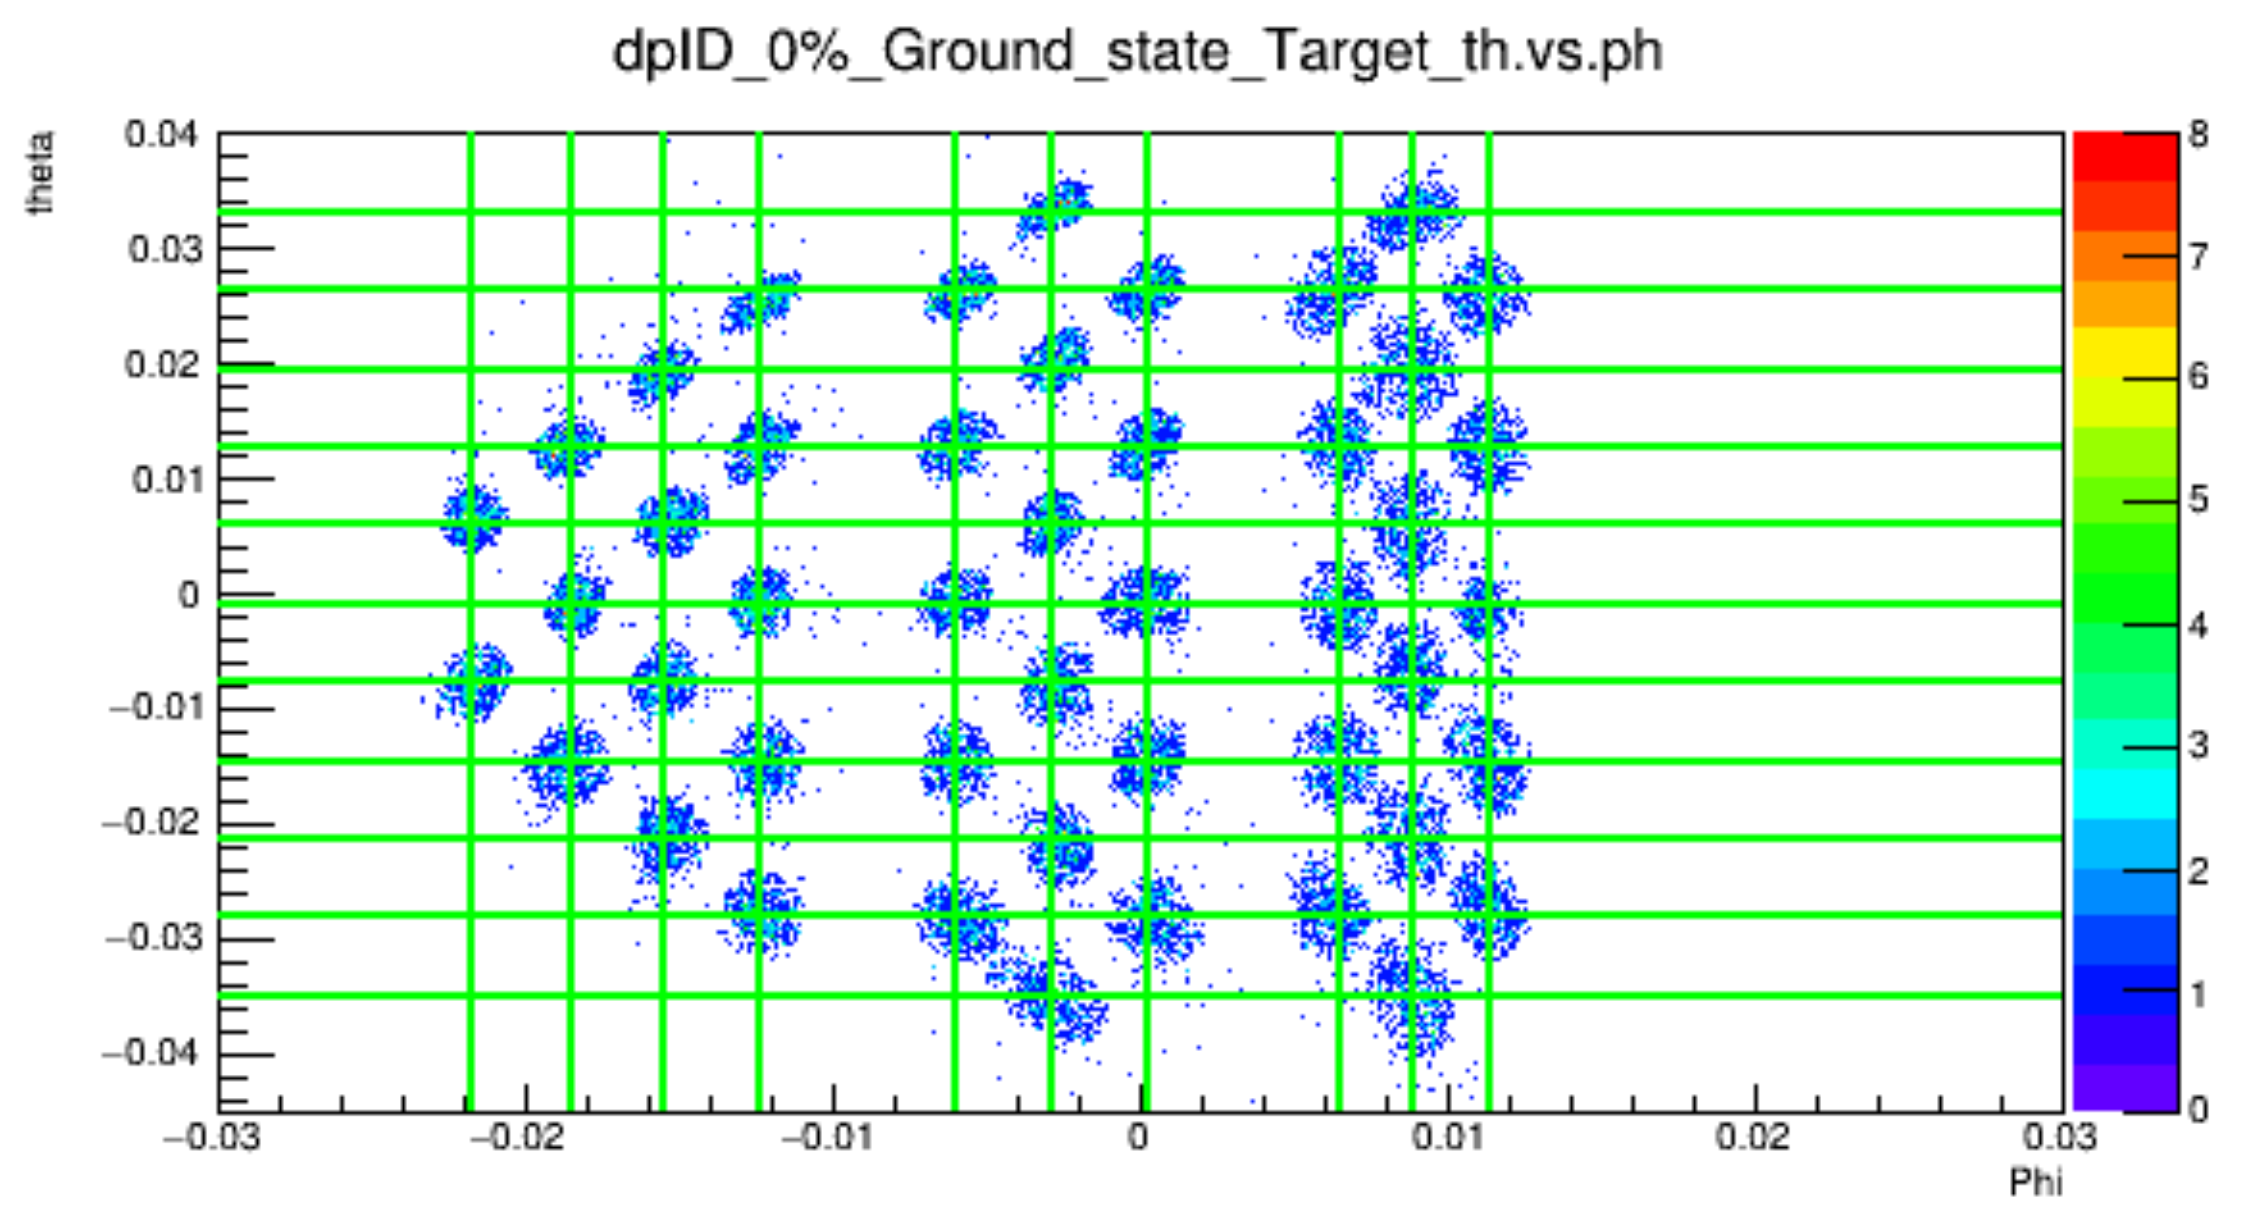
\includegraphics[width =\textwidth]{images/chap4/LHRS_tg_theta_phi_after_opt.png}
    \caption{LHRS Target $\theta_{tg}$ vs. $\phi_{tg}$ on target coordinate system}
    \label{fig:lhrs_tg_theta_phi_postopt}
\end{figure}

\begin{figure}[h]
    \centering
    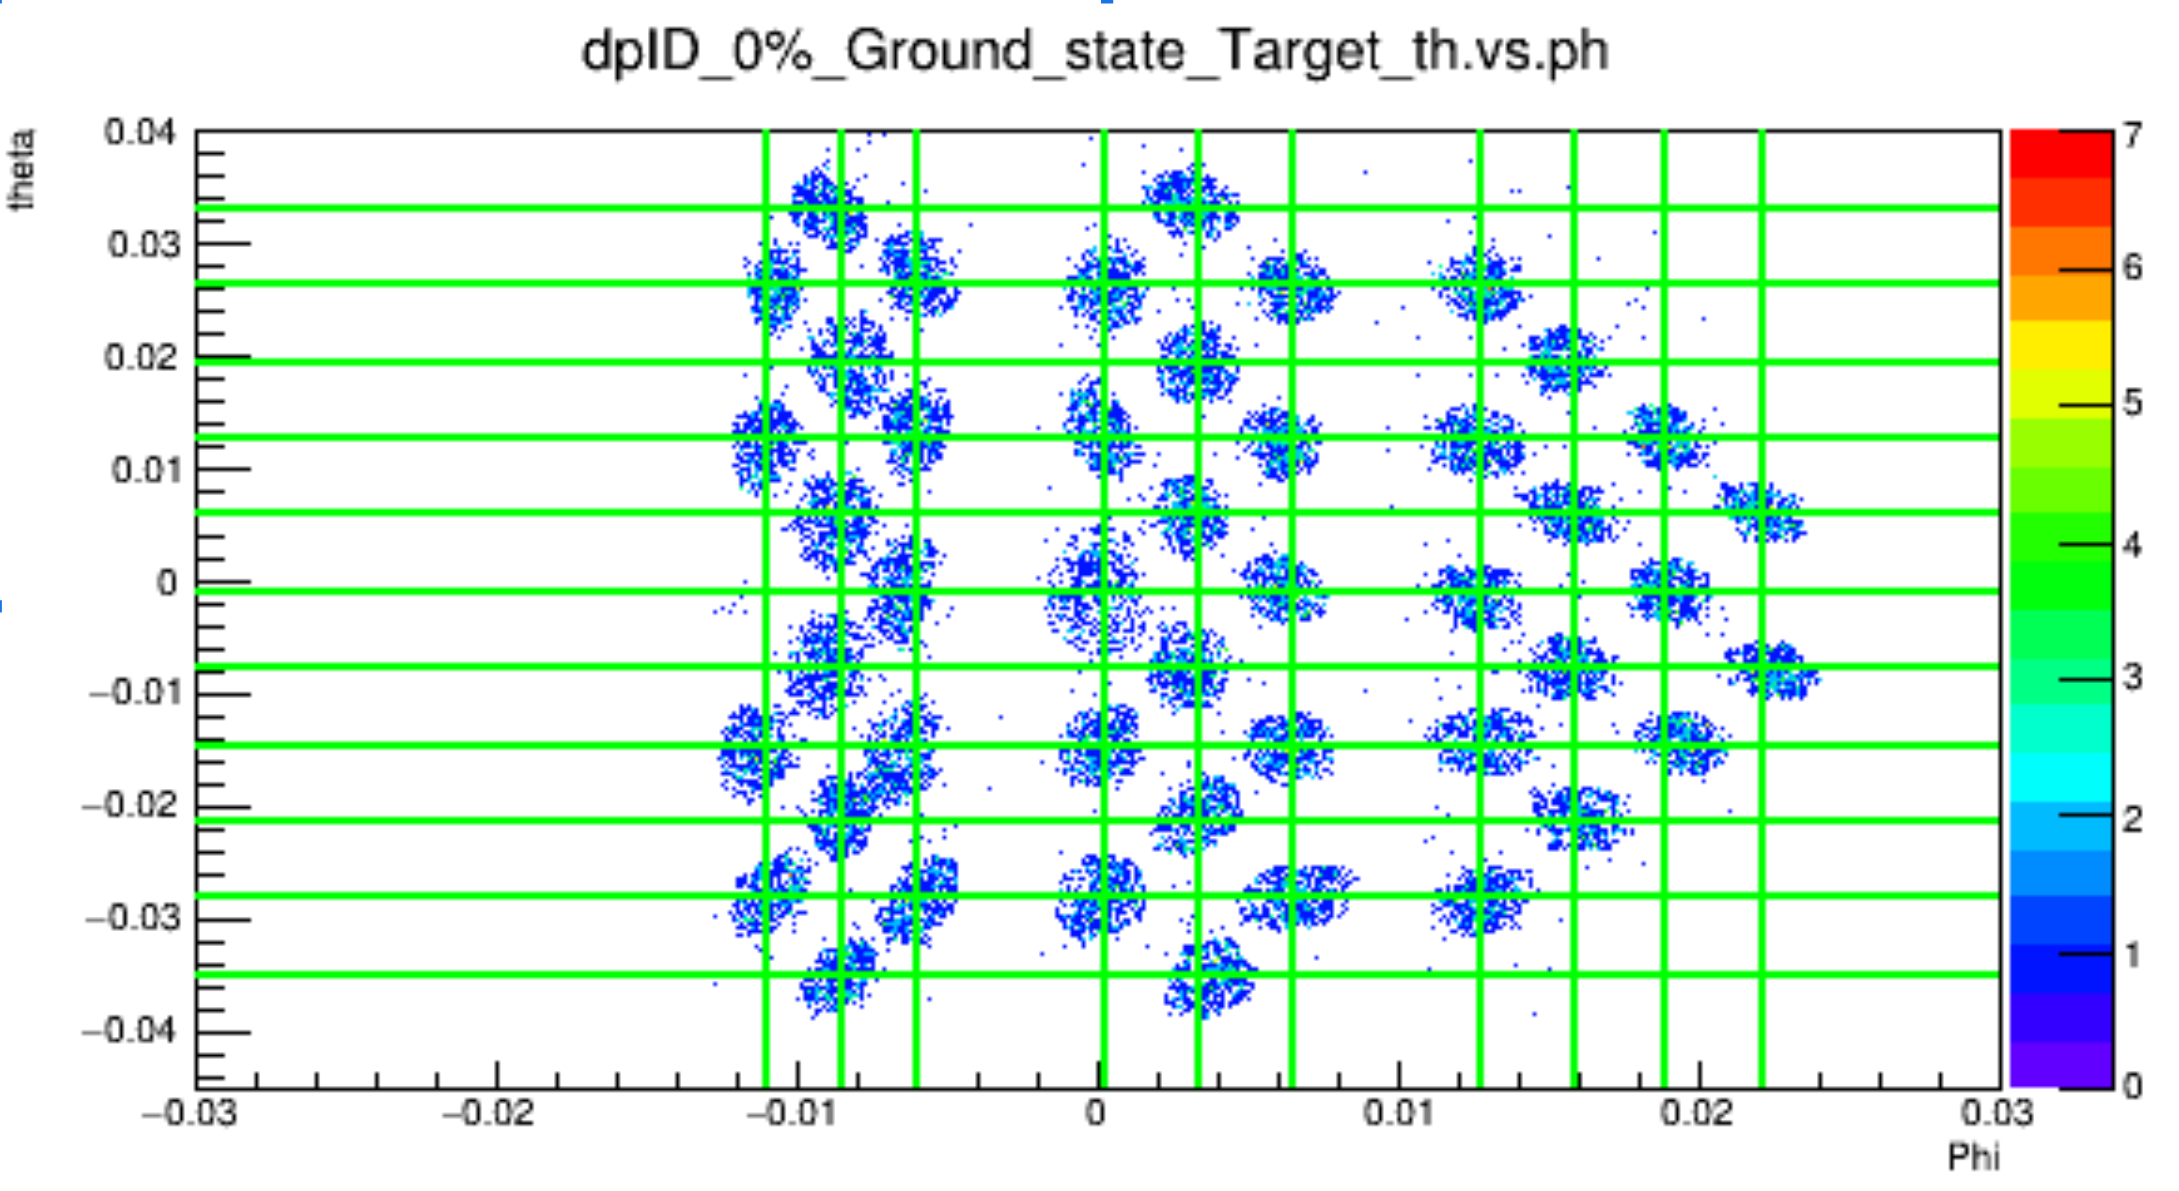
\includegraphics[width =\textwidth]{images/chap4/rhrs_tg_theta_phi_after_opt.png}
    \caption{RHRS Target $\theta_{tg}$ vs. $\phi_{tg}$ on target coordinate system}
    \label{fig:rhrs_tg_theta_phi_postopt}
\end{figure}

\begin{figure}[h]
    \centering
    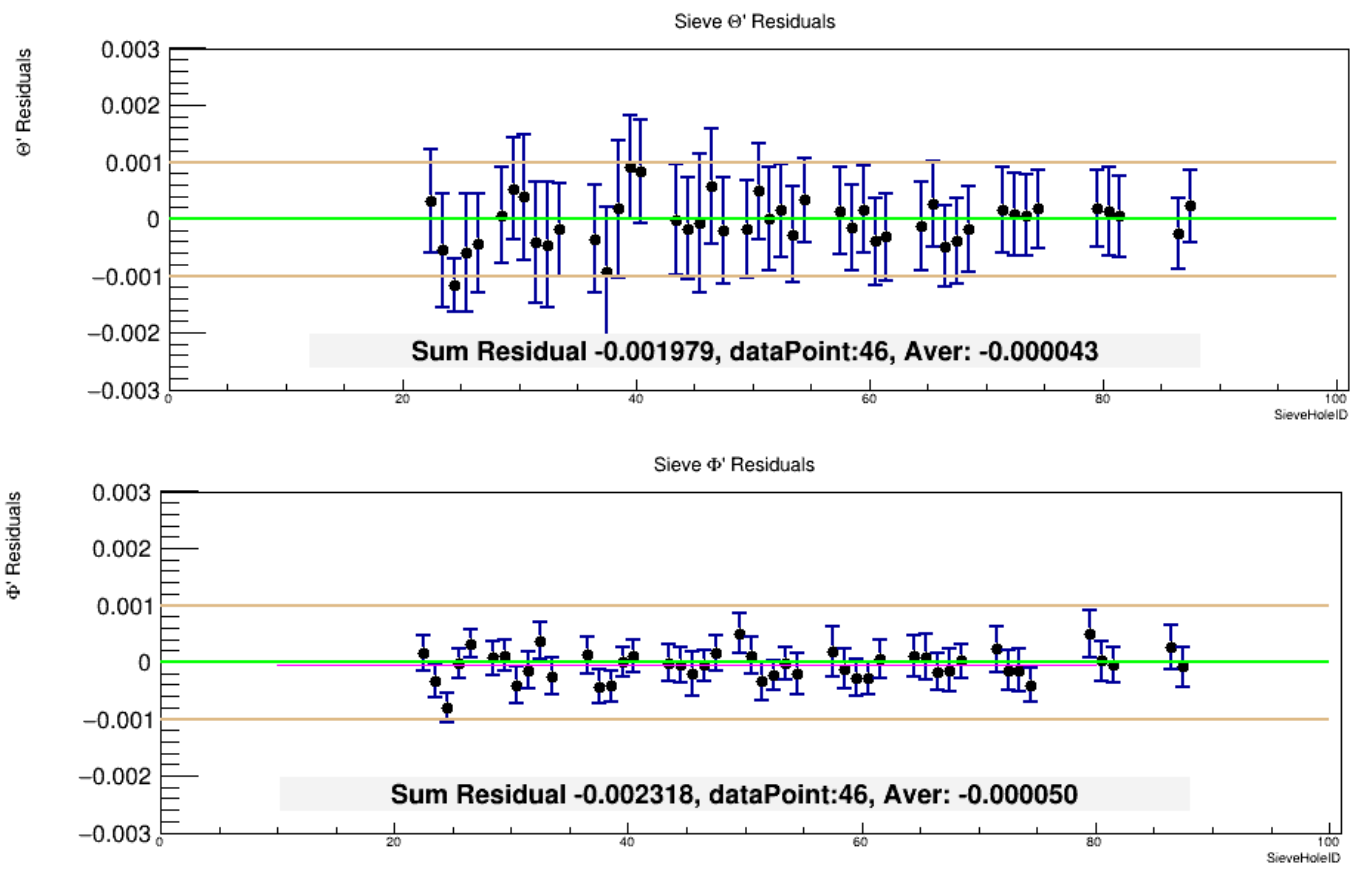
\includegraphics[width =\textwidth]{images/chap4/lhrs_tg_residual_plot.png}
    \caption{LHRS Target $\theta_{tg}$ and $\phi_{tg}$ Optimization Residual on Target Coordinate System}
    \label{fig:lhrs_tg_theta_phi_residual}
\end{figure}

\begin{figure}[h]
    \centering
    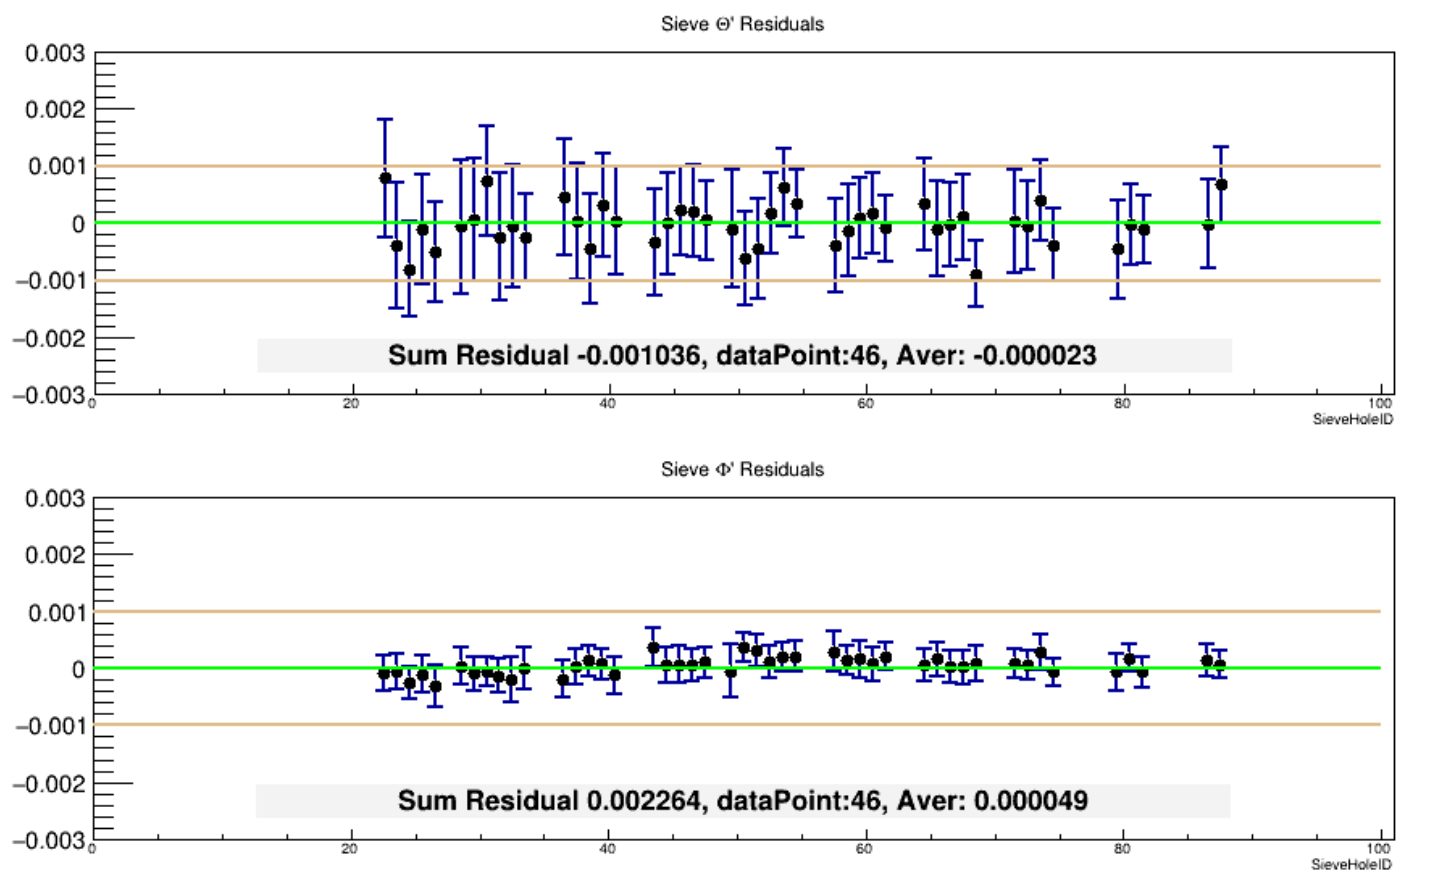
\includegraphics[width =\textwidth]{images/chap4/rhrs_residual_theta_phi.png}
    \caption{RHRS Target $\theta_{tg}$ and $\phi_{tg}$ Optimization Residual on Target Coordinate System}
    \label{fig:rhrs_tg_theta_phi_residual}
\end{figure}

\begin{center}
    \begin{tabular}{|c || c | c|}
        \hline
        \multicolumn{3}{|c|}{Angular Variable Calibration Accuracy} \\
        \hline
            HRS & $\theta$ & $\phi$ \\
        \hline
            RHRS & -1.57 mrad & 0.32 mrad \\
        \hline
            LHRS & 0.732 mrad & -0.492 mrad \\
            \hline
    \end{tabular}
\end{center}

\subsection{Momentum Calibration}
\subsubsection{Momentum Ground truth}

The scattering angle represents the angle between the direction of the scattered electrons and the direction of the electron beam. Standard survey procedures do not directly measure the scattering angle; instead, they measure the spectrometer central angle and the geometric positions of the sieve plate. The scattering angle can be calculated using the spectrometer central angle and the $\theta_{tg}$ and $\phi_{tg}$, which are determined based on the geometric position of the sieve hole relative to the central sieve hole. Given these parameters, the scattering angle can be calculated as:

\begin{equation} \label{eq:chapter4_scattered_angle_from_central_angle}
\theta = \frac{\cos{\theta_0} - \phi_{tg}\sin{\theta_0}}{\sqrt{1 + \theta^2_{tg} + \phi^2_{tg}}}
\end{equation}

With the scattering angle, the ground truth scattered electron momentum can be calculated as:

\begin{equation}
 p = \frac{E}{1 + \frac{2E}{M_c}(1 - \cos{\theta})}
\end{equation}


\subsubsection{Momentum Calibration result}
As stated in the equations, to simplify the complexity and facilitate model conversion, the momentum calibration is optimized using $\delta = \frac{p - p_0}{p_0}$. Similar to $\theta$ and $\phi$, the optimization needs to be performed separately for the LHRS and RHRS. The ground truth value incorporates the central sieve angle and the angle of the sieve hole in the target coordinate system within the sieve plate. The L2 loss function is employed, which calculates the sum of squared residuals between the ground truth $\delta p$ and the $\delta p$ computed using the projected momentum with the HRS tensor.

To cover a broader momentum range, data are taken with central momenta at $-1\%$, $0\%$, and $1\%$ of the standard central sieve momentum. Figures \ref{fig:lhrs_dp_residual} and \ref{fig:rhrs_dp_residual} display the residuals for LHRS and RHRS. Similar to the sieve $\theta$ and $\phi$ residual plots, data are grouped by the sieve hole. The beam energy of the accelerator is $952.9 MeV$.

The table below presents the error bars for the momentum optimization. The error is considered to be the largest residual difference compared to the theoretical value.

\begin{center}
    \begin{tabular}{|c || c |}
        \hline
        \multicolumn{2}{|c|}{Momentum Calibration Accuracy} \\
        \hline
            HRS & Momentum Error \\
        \hline
            RHRS & $\pm 0.5MeV$ \\
        \hline
            LHRS & $\pm 0.3MeV$ \\
        \hline
    \end{tabular}
\end{center}


\begin{figure}[h]
    \centering
    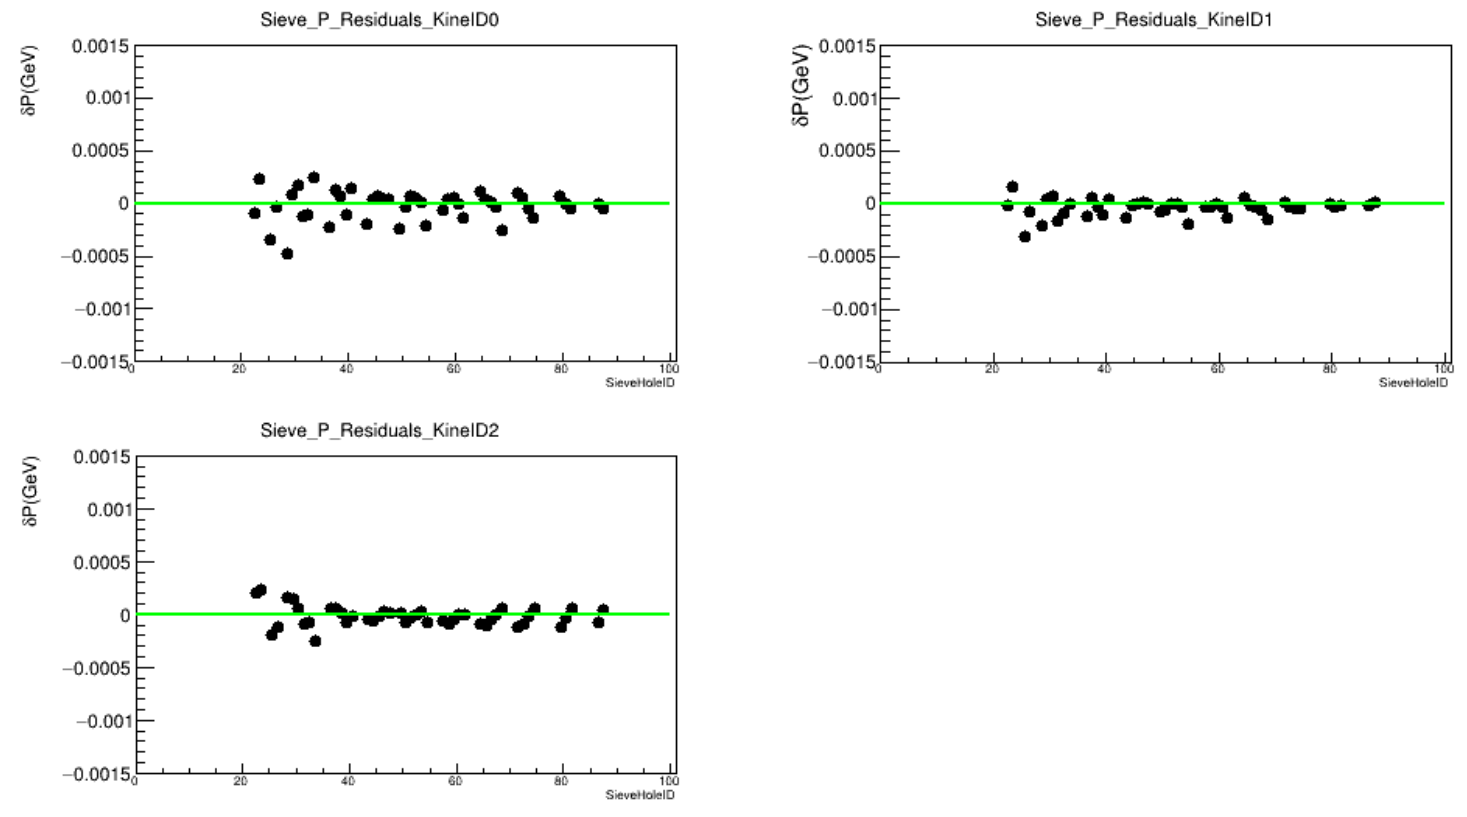
\includegraphics[width =\textwidth]{images/chap4/lhrs_dp_residual.png}
    \caption{Caption}
    \label{fig:lhrs_dp_residual}
\end{figure}


\begin{figure}[h]
    \centering
    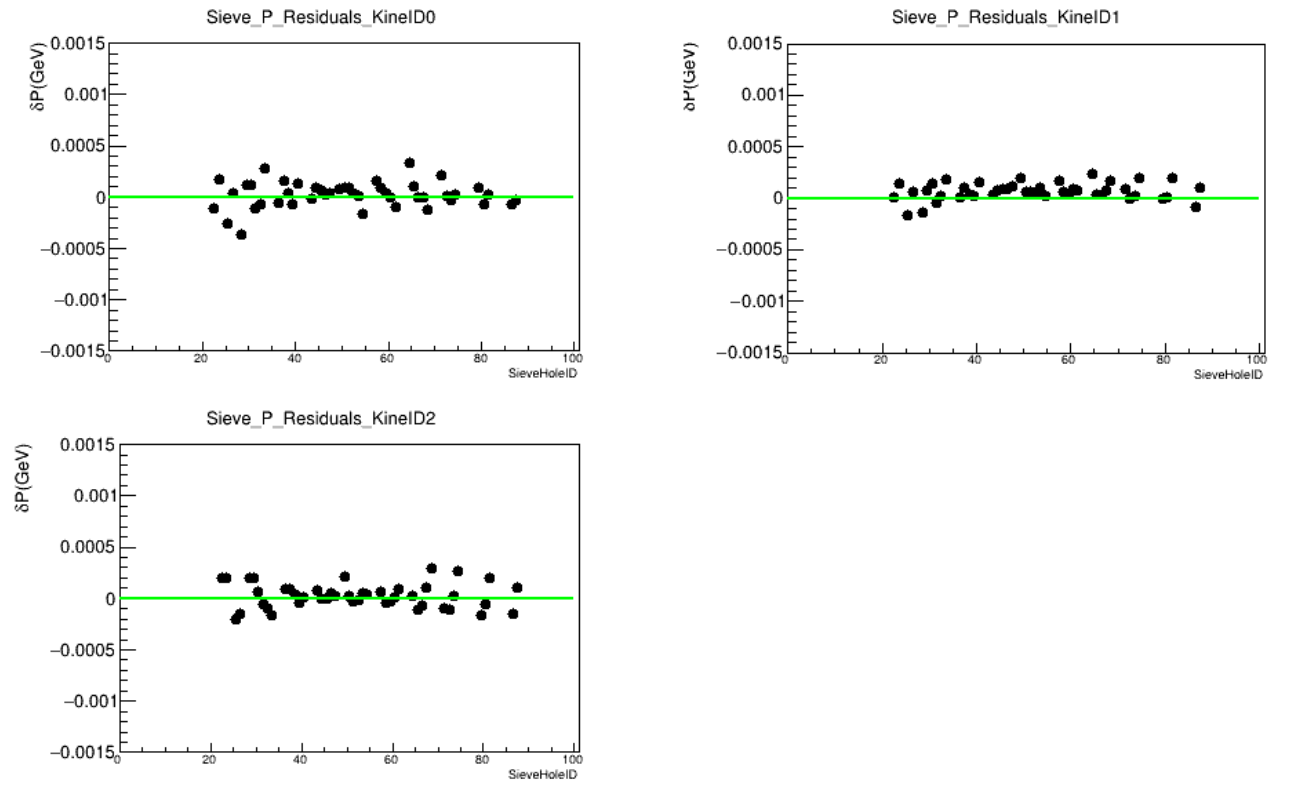
\includegraphics[width =\textwidth]{images/chap4/rhrs_dp_residual.png}
    \caption{Caption}
    \label{fig:rhrs_dp_residual}
\end{figure}

\section{Spectrometer central angle $\theta_0$ measurement }

The spectrometer central angle, $\theta_0$, is defined as the angle between the beam down direction and the central spectrometer axis. As shown in equation \ref{eq:chapter4_scattered_angle_from_central_angle}, the spectrometer's central angle serves as a fundamental input for calculating the particle scattered angle. The laser survey provides the spectrometer's central angle. $\theta_0$ can be measured using a survey that measures the angle between two imaginary lines: the first line runs along the ideal spectrometer axis, and the second line runs along the ideal electron beam direction.

However, multiple transformations are required to relate the ideal spectrometer angle to the actual spectrometer angle, which could increase the uncertainty of the $\theta_0$ measurement to as much as 0.06 or approximately $1\%$. This could, in turn, lead to a $2\%$ uncertainty in Q2 measurement in the case of the PREX experiment. In PRex Experiment, the measurement is through pointing measurement. This technique utilizes the concept of differential nuclear recoil for elastic electron scattering off target nuclei of different masses. Pointing measurements are generally more accurate than surveys, as they do not require multiple transformations like surveys. Furthermore, the accuracy of pointing measurements can be significantly improved by considering differential nuclear recoils off different target nuclei present in the same target, such as water (H2O). This method has the advantages of suppressing uncertainties from estimating energy losses occurring before and after scattering and eliminating the issue of potential beam position shifting during the run. The primary uncertainty that contributes to the pointing measurement uncertainty arises from the ability to measure the energy difference between two different peaks. In the case of PREX, the accuracy was at the level of ~30 keV. [change needed]

Consider an electron scattered on a target with mass $M$. The scattered electron momentum can be written as:

\begin{equation}
E' = \frac{E - E_{loss1}}{1 + \frac{2(E-E_{loss1})\sin^2{\frac{\theta}{2}}}{M}} - E_{loss2}
\end{equation}

In this equation, $E$ represents the initial energy of the electrons, $\theta$ is the scattered angle, $E_{loss1}$ is the energy loss occurring before scattering, and $E_{loss2}$ is the energy loss occurring after scattering.

The water target contains both $^{1}H$ and $^{16}O$, enabling the scattering of two targets with precisely the same beam energy, scattered angle, and energy loss. The energy loss is canceled out, thus increasing the measurement accuracy. The scattered electron energy difference between oxygen and hydrogen can be given by:

\begin{equation}
\Delta{E'} = E'_O - E'_H = E (\frac{1}{1 + \frac{2E\sin^2{\frac{\theta}{2}}}{M_O}} - \frac{1}{1 + \frac{2E\sin^2{\frac{\theta}{2}}}{M_H}}) + corrections
\end{equation}

In this equation, the corrections are negligible. Both the beam energy and the masses of oxygen and hydrogen are measured with high accuracy. With the scattered momentum reconstructed from the vertical drift chamber and the above equation, the scattered angle can be measured.

The CRex experiment uses the exact same spectrometer configuration, but with a beam energy of 2.18 GeV, yielding a much cleaner energy spectrum. In data analysis, CRex data is used instead of PREX data to achieve higher accuracy measurements.

The pointing measurement was conducted with a sieve in place, and events passing through the central sieve hole were used in the pointing calculation with the beam position along the center of the Hall A Coordinate System. This approach eliminates errors caused by HRS optics reconstruction errors. Figure \ref{fig:pointing_h2o_spectrum} displays an example of the waterfall target spectrum for CRex RHRS run 21737. The first peaks on the left and right represent the ground state energies of $^{1}H$ and $^{16}O$, respectively. The energy difference is $\Delta E = 16.126 \pm 0.024 MeV$. In order to obtain a highly accurate central angle, the pointing measurements were performed with different central momenta. The scattered electrons will end up in different VDC areas with different central momenta. Each central momentum run can provide independent energy differences between the hydrogen and oxygen spectra. Accurate optics reconstruction allows different central momenta to yield different energy differences between the hydrogen and oxygen targets while maintaining the same scattering angles. This helps verify the calibration accuracy.

To avoid drift during the experiment, pointing measurements were conducted three times: once at the beginning, once during the experiment, and a final verification pointing measurement after the experiment. The final pointing measurement is the average of these runs. A table listing all the runs used in the pointing measurement is provided.

During the pointing process, although the beam position is set to (0,0), it cannot perfectly reach $(0,0)$ due to control errors. To account for errors caused by beam position, the final angle is corrected by $\frac{X_{bpm}}{Z_0}$, where $Z_0$ represents the distance from the target center to the sieve slide along the spectrometer central ray (verification required), and $X_{bpm}$ is the beam position in the $X$ direction in the Hall A coordinate system.  

\begin{table}[!ht]
    \caption{LHRS Dec-16-2019 Pointing measurement}
    \centering
    \begin{tabular}{|l|l|l|l|l|l|}
    \hline
        ~ & LHRS & Initial\_L & bpmX & Correct Angle & Corrected HRS \\ \hline
       \multirow{5}{5em}{Dp $0\%$} &  2671 & 4.771 & 1.070 & -0.062 & 4.833 \\  
        ~ & 2672 & 4.831 & 0.083 & -0.005 & 4.836 \\ 
        ~ & 2673 & 4.725 & 2.011 & -0.116 & 4.841 \\ 
        ~ & 2674 & 4.763 & 1.081 & -0.062 & 4.825 \\  
        ~ & 2675 & 4.787 & 1.008 & -0.058 & 4.845 \\ \hline
        \multirow{3}{5em}{ Dp $+1\%$} & 2709 & 4.749 & 0.936 & -0.054 & 4.803 \\ 
        ~ & 2710 & 4.806 & 0.094 & -0.005 & 4.811 \\  
        ~ & 2711 & 4.691 & 2.049 & -0.118 & 4.809 \\ \hline
        \multirow{5}{5em}{ Dp $-1\%$} & 2723 & 4.755 & 0.950 & -0.055 & 4.810 \\   
        ~ & 2724 & 4.808 & -0.029 & 0.002 & 4.806 \\  
        ~ & 2725 & 4.702 & 2.055 & -0.119 & 4.821 \\ 
        ~ & 2726 & 4.756 & 1.093 & -0.063 & 4.819 \\  
        ~ & 2727 & 4.771 & 1.017 & -0.059 & 4.830 \\ \hline
    \end{tabular}
    \label{table:crex_1_pointing_lhrs}
\end{table}


\begin{table}[!ht]
    \caption{RHRS Dec-16-2019 Pointing measurement}
    \centering

    \begin{tabular}{|l|l|l|l|l|l|}
    \hline
        ~ & RHRS & Initial\_R & bpmX & Correct Angle & Corrected HRS \\ \hline
        \multirow{5}{5em}{Dp $0\%$} & 21736 & 4.771 & 1.070 & 0.062 & 4.709 \\
        ~ & 21737 & 4.722 & 0.083 & 0.005 & 4.717 \\
        ~ & 21738 & 4.827 & 2.011 & 0.116 & 4.711 \\
        ~ & 21739 & 4.78 & 1.081 & 0.062 & 4.718 \\
        ~ & 21740 & 4.78 & 1.008 & 0.058 & 4.722 \\ \hline
        \multirow{3}{5em}{ Dp $+1\%$} & 21774 & 4.749 & 0.936 & 0.054 & 4.695 \\
        ~ & 21775 & 4.706 & 0.094 & 0.005 & 4.701 \\
        ~ & 21776 & 4.813 & 2.049 & 0.118 & 4.695 \\ \hline
        \multirow{5}{5em}{ Dp $-1\%$} & 21786 & 4.757 & 0.950 & 0.055 & 4.702 \\ 
        ~ & 21787 & 4.692 & -0.029 & -0.002 & 4.694 \\ 
        ~ & 21788 & 4.806 & 2.055 & 0.119 & 4.687 \\
        ~ & 21789 & 4.752 & 1.093 & 0.063 & 4.689 \\ 
        ~ & 21790 & 4.75 & 1.017 & 0.059 & 4.691 \\ \hline
    \end{tabular}
    \label{table:crex_1_pointing_lhrs}
\end{table}


\begin{table}[!ht]
    \caption{LHRS Aug-9-2020 Pointing measurement}
    \centering
    \begin{tabular}{|l|l|l|l|l|l|}
    \hline
        ~ & LHRS & Initial\_L & bpmX & corrected\_A & Corrected HRS \\ \hline
        \multirow{5}{5em}{Dp $0\%$} & 3108 & 4.716 & 1.981 & -0.1143 & 4.8303 \\  
        ~ & 3109 & 4.832 & 0.045 & -0.0026 & 4.8346 \\ 
        ~ & 3110 & 4.832 & 0.006 & -0.0003 & 4.8323 \\  
        ~ & 3111 & 4.713 & 1.896 & -0.1094 & 4.8224 \\  
        ~ & 3112 & 4.785 & 0.963 & -0.0555 & 4.8405 \\  \hline
        \multirow{2}{5em}{Dp $-1\%$} & 3113 & 4.758 & 0.980 & -0.0565 & 4.8145 \\ 
        ~ & 3114 & 4.754 & 0.989 & -0.0571 & 4.8111 \\ \hline
    \end{tabular}
    \label{table:crex_2_pointing_lhrs}
\end{table}

\begin{table}[!ht]
    \caption{RHRS Aug-9-2020 Pointing measurement}
    \centering
    \begin{tabular}{|l|l|l|l|l|l|}
    \hline
        ~ & RHRS & Initial\_R & bpmX & Correct Angle & Corrected HRS \\ \hline
        \multirow{5}{5em}{Dp $0\%$} & 22114 & 4.842 & 1.981 & 0.114 & 4.728 \\ 
        ~ & 22115 & 4.734 & 0.045 & 0.003 & 4.731 \\  
        ~ & 22116 & 4.743 & 0.006 & 0.000 & 4.743 \\  
        ~ & 22117 & 4.853 & 1.896 & 0.109 & 4.744 \\  
        ~ & 22118 & 4.788 & 0.963 & 0.056 & 4.732 \\ \hline
        \multirow{2}{5em}{Dp $-1\%$} & 22119 & 4.769 & 0.980 & 0.057 & 4.712 \\ 
        ~ & 22120 & 4.767 & 0.989 & 0.057 & 4.710 \\ \hline
    \end{tabular}
    \label{table:crex_2_pointing_rhrs}
\end{table}

\begin{table}[!ht]
    \caption{LHRS Sep-13-2020 Pointing measurement}
    \centering
    \begin{tabular}{|l|l|l|l|l|l|}
    \hline
        ~ & LHRS & Initial\_L & bpmX & corrected\_A & Corrected HRS \\ \hline
        \multirow{5}{5em}{Dp $0\%$} & 3278 & 4.773 & 0.985 & -0.057 & 4.830 \\  
        ~ & 3279 & 4.83 & 0.069 & -0.004 & 4.834 \\  
        ~ & 3284 & 4.721 & 2.007 & -0.116 & 4.837 \\  
        ~ & 3286 & 4.771 & 1.057 & -0.061 & 4.832 \\ 
        ~ & 3291 & 4.776 & 1.006 & -0.058 & 4.834 \\ \hline
        \multirow{2}{5em}{Dp $+1\%$}  & 3292 & 4.8 & 1.035 & -0.060 & 4.860 \\  
        ~ & 3299 & 4.802 & 1.049 & -0.060 & 4.862 \\ \hline
        \multirow{1}{5em}{Dp $-1.7\%$} & 3302 & 4.738 & 1.052 & -0.061 & 4.799 \\ \hline
    \end{tabular}
    \label{table:crex_3_pointing_lhrs}
\end{table}


\begin{table}[!ht]
    \caption{RHRS Sep-13-2020 Pointing measurement}
    \centering
    \begin{tabular}{|l|l|l|l|l|l|}
    \hline
        ~ & RHRS & Initial\_R & bpmX & Correct Angle & Corrected HRS \\ \hline
        \multirow{5}{5em}{Dp $0\%$} & 22234 & 4.789 & 0.985 & 0.057 & 4.732 \\ 
        ~ & 22235 & 4.741 & 0.069 & 0.004 & 4.737 \\ 
        ~ & 22240 & 4.849 & 2.007 & 0.116 & 4.733 \\ 
        ~ & 22242 & 4.812 & 1.057 & 0.061 & 4.751 \\  
        ~ & 22247 & 4.793 & 1.006 & 0.058 & 4.735 \\ \hline
        \multirow{2}{5em}{Dp $+1\%$} & 22248 & 4.791 & 1.035 & 0.060 & 4.731 \\ 
        ~ & 22255 & 4.786 & 1.049 & 0.060 & 4.726 \\ \hline
        \multirow{1}{5em}{Dp $-1.7\%$} & 22256 & 4.743 & 1.052 & 0.061 & 4.682 \\ \hline
    \end{tabular}
    \label{table:crex_3_pointing_rhrs}
\end{table}

\begin{figure}[h]
    \centering
    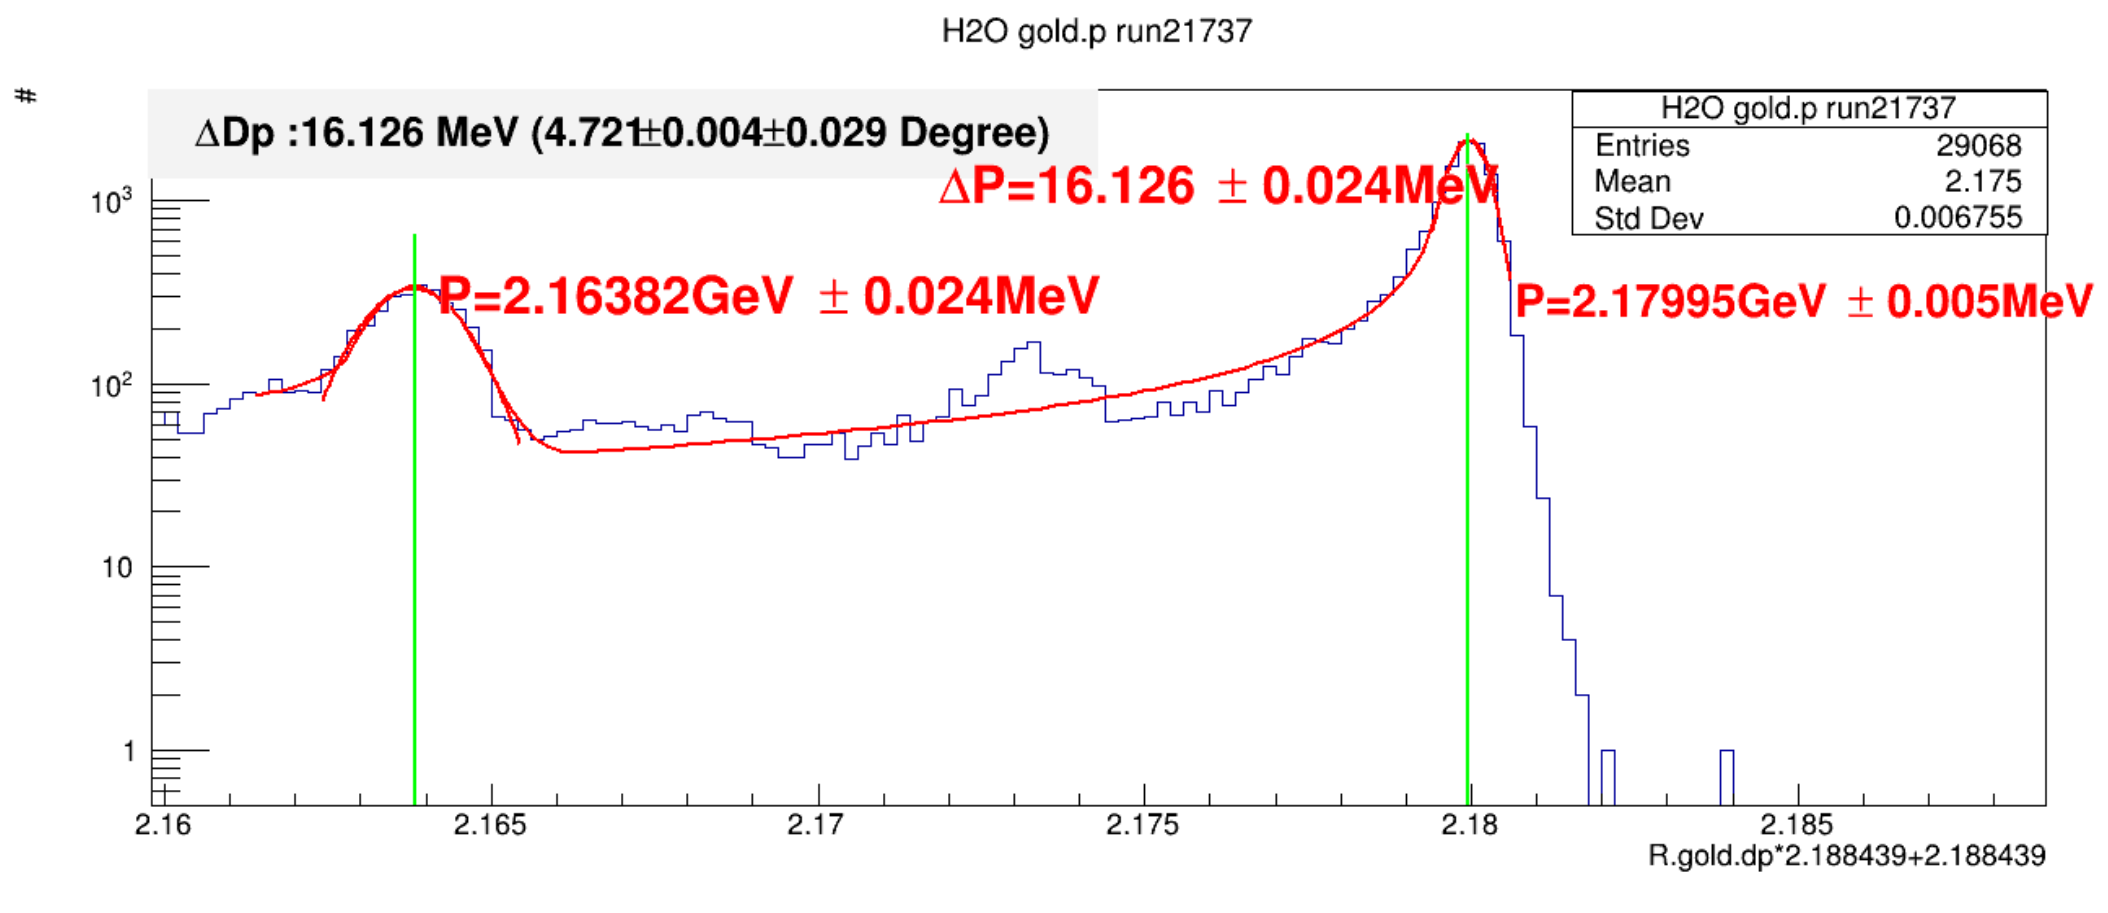
\includegraphics[width =\textwidth]{images/chap4/pointing_h20_spectrum.png}
    \caption{Caption}
    \label{fig:pointing_h2o_spectrum}
\end{figure}


\begin{figure}[h]
    \centering
    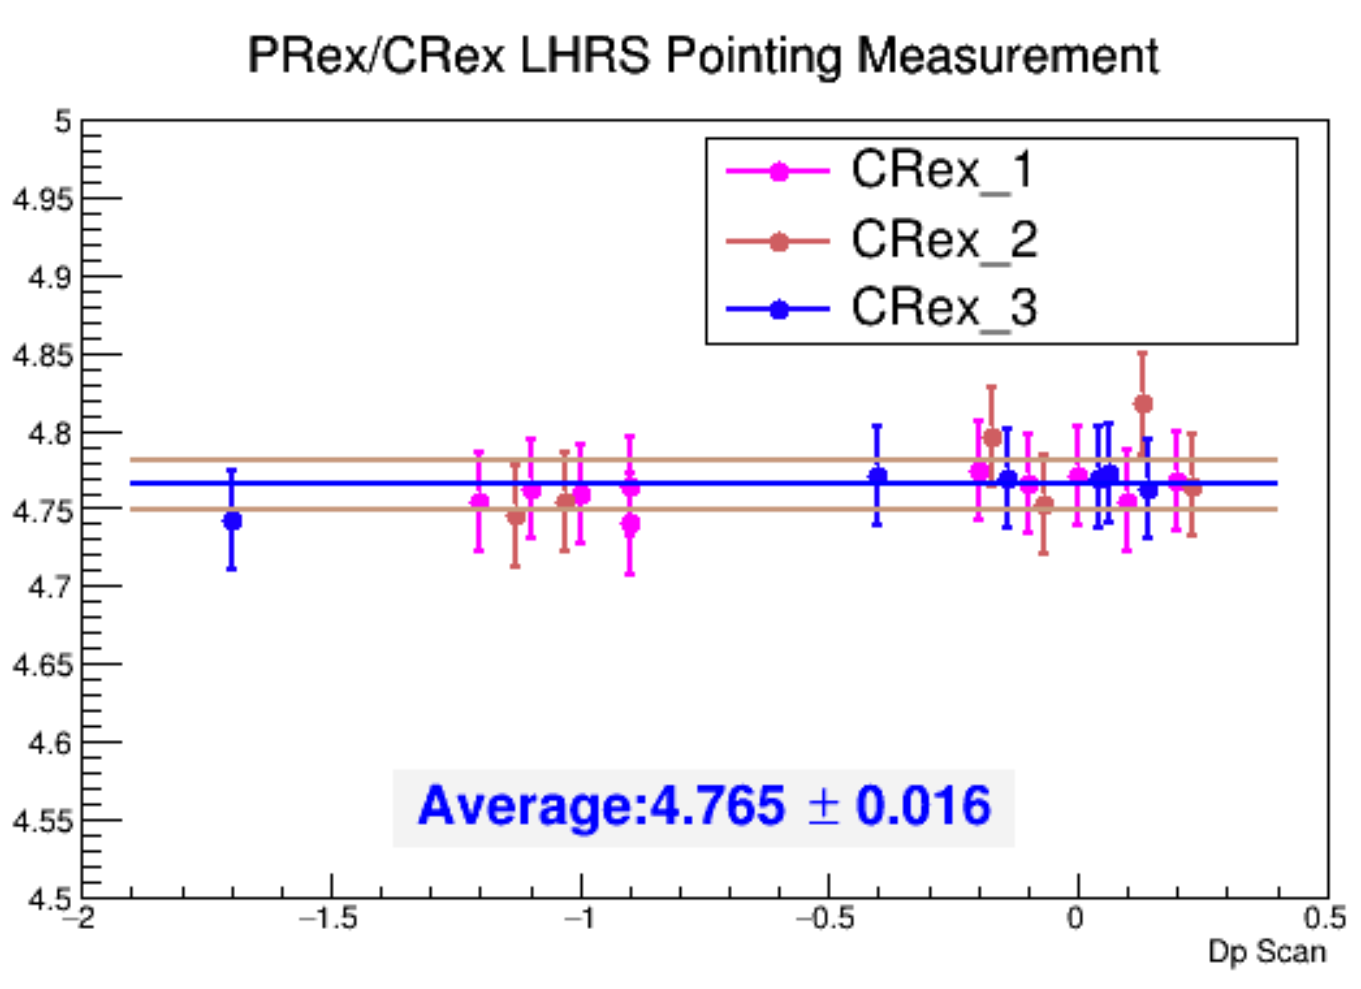
\includegraphics[width =\textwidth]{images/chap4/lhrs_pointing_summary.png}
    \caption{Caption}
    \label{fig:my_label}
\end{figure}

\begin{figure}[h]
    \centering
    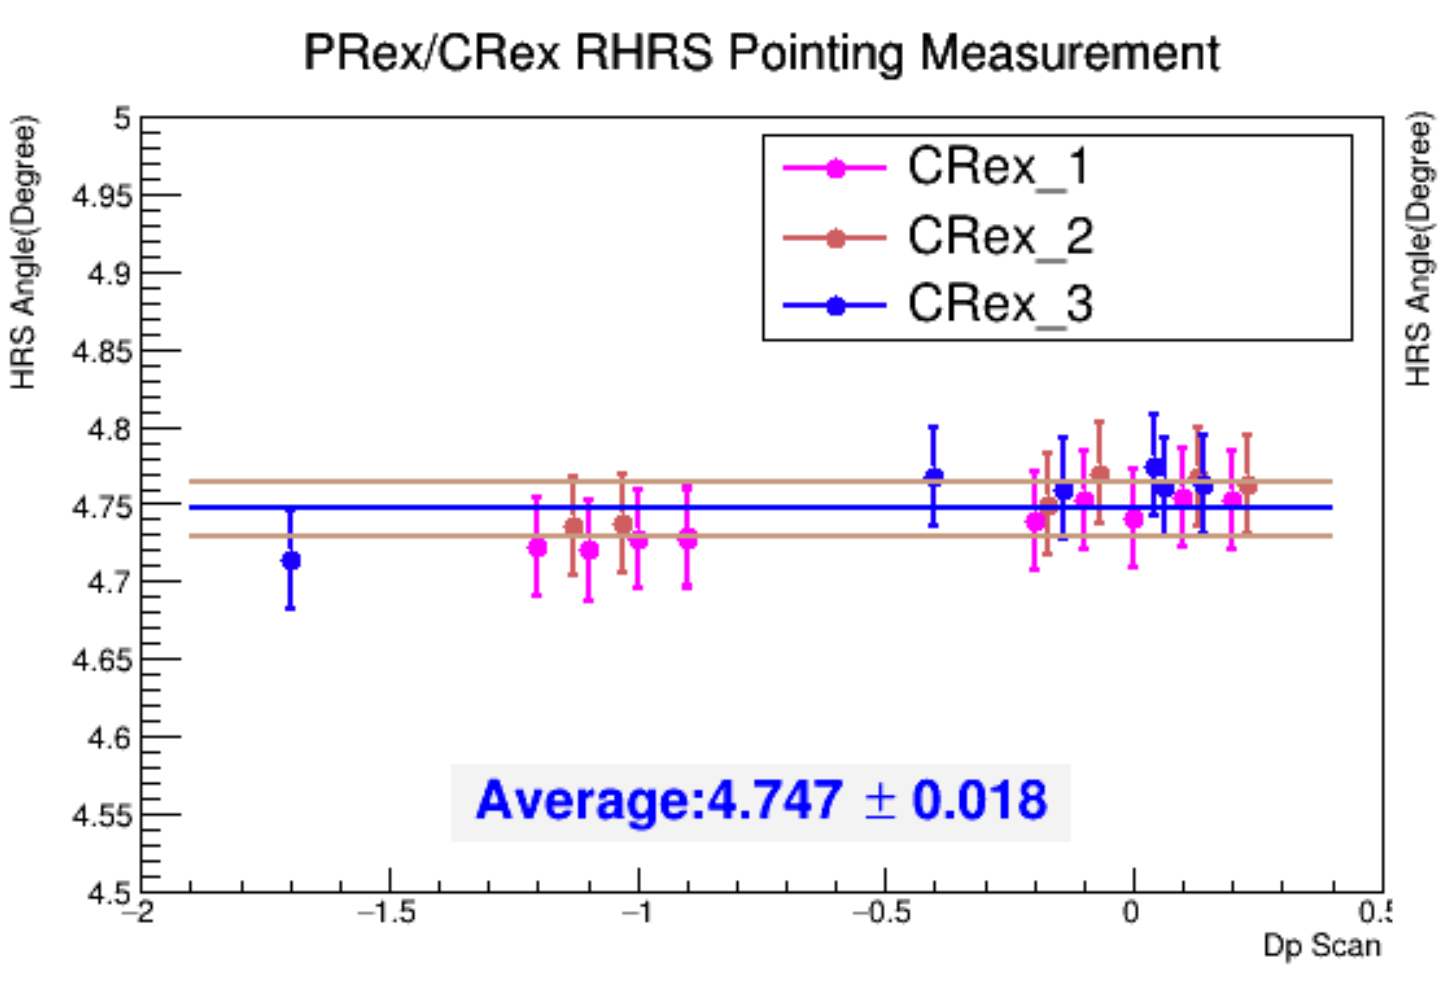
\includegraphics[width =\textwidth]{images/chap4/rhrs_pointing_summary.png}
    \caption{Caption}
    \label{fig:my_label}
\end{figure}

\hyperlink{https://docs.google.com/spreadsheets/d/12B7BL0aG4ZT-L9QYeQnX1PDxArS75PFv40Hdc3eRv4k/edit?usp=sharing}{data source, need to add that information}

\hyperlink{https://github.com/Jiansiyu/GeneralScripts/blob/master/PointingCheck/crex_pointing.csv}{Pointing measurement final result csv}




% \subsubsection{beam position correction}

% \subsection{CRex experiment calibration}
% \subsection{a second thought on the optics optimization}


% Move to a separate chapter describing the apparatus and experiment details

% \begin{itemize}
%     \item Overview of the HRS structure
%     \item septum magnet 
%     \item Vertical drift chamber 
%     \item GEM detector
%     \item supporting equipment used for optimization only sieve slide

%     \item coordination system of the Jefferson Lab Hall A
%     \item coordination system of the HRS
% \end{itemize}


% \subsection{HRS model}

% \begin{itemize}
%     \item mathematical model of the HRS
%     \item constant parameter optimization
%     \item Vertical Drift Chamber time optimization
%     \item carbon calibration(dashed lines in the VDC spectrometer)
%     \item math why higher order contribute, a discussion notes
%     \item feature selection techniques
%     \item linear regression
%     \item result validation
%     \item result and discussion
% \end{itemize}
% \subsubsection{supervised linear regression}
% \subsubsection{feature selection technics}
% \subsubsection{mathematics about the linear regression, LASSO and ridge regression}

% \subsubsection{Linear Regression and mathematics approximation}




% \subsection{}section{feature selection}

% \subsubsection{general consideration in regression}

% \subsubsection{features in regression}

% \subsubsection{LASSO feature reduction regression}

% \subsubsection{ridge feature reduction regression}

% \subsection{autoML and more}

% \section{Momentum optimization}

% \section{Regression Result validation}

% \subsection{carbon result check}

% \subsubsection{first, second, third momentum check}

% \section{momentum reconstruction}

% \section{scattered angle reconstruction and correction}

% \section{a second thought/attempt on the regression}

% \subsection{another more complicated model}
\chapter{GEM detector @ HRS}
\subsection{VDC}
\subsection{GEM detector Data Analysis}
\subsubsection{current GEM apparatus}
\subsubsection{GEM detector data structure}
\subsubsection{GEM detector alignment}
\subsubsection{GEM detector performance, and efficiency change via the time}
\subsection{$Q^2$ calculation}
\subsection{$r$ calculation with the data}
% \lipsum[1-20]

\chapter{Result and Conclusions}

\section{Result of PRex-II experiment}

The PRex-II experiment measures the neutron skin thickness with the parity violated electron scattering. The PRex-II experiment was carried out at Jefferson Lab Hall A with the High-resolution spectrometer. The experiment was performed at a beam energy of 0.95 GeV/c and collected 114 coulombs of charges. 



\begin{itemize}
    \item equations
    \item APV
    \item R_w
    \item symmetry energy (L)
    \item skin thickness 
\end{itemize}


\begin{itemize}
    \item PRex experiment was carried out in jlab 
    \item energy 
    \item  beam current 
    \item  This chapter will introduce about result 
    \item use the skin thickness to get the neutron star, EOS, L 
\end{itemize}

\begin{itemize}
    \item run info
    \item beam info
    \item beam energy 
    \item beam current 
\end{itemize}


\begin{itemize}
    \item measurement errors for each parts
    \item beam polarization 
    \item APV
\end{itemize}

Para. table of different measurement errors (refer)

\begin{table}[]
    \centering
    \begin{tabular}{c c c} \\ 
    \hline
         Correction     & Absolute [ppb] & Relative [$\%$]  \\ \hline
         Beam asymmetry & $-60.4 \pm 3.0$ & $11.0 \pm 0.5$ \\ 
         Charge correction & $20.7 \pm 0.2$ & $3.8 \pm 0.0$ \\
         Beam polarization & $56.8 \pm 5.2$ & $10.3 \pm 1.0$ \\
         Target diamond foils & $0.7 \pm 1.4$ & $0.1 \pm 0.3$ \\
         Spectrometer rescattering & $0.0 \pm 0.1$ & $0.0 \pm 0.0$ \\
         Inelastic contribution & $0.0 \pm 0.1$ & $0.0 \pm 0.0$ \\
         Transverse asymmetry & $0.0 \pm 0.3$ & $0.0 \pm 0.1$ \\
         Detector nonlinearity & $0.0 \pm 2.7$ & $0.0 \pm 0.5$ \\
         Angle determination & $0.0 \pm 3.5$ & $0.0 \pm 0.6$ \\
         Acceptance function & $ 0.0 \pm 2.9$ & $0.0 \pm 0.5$ \\
         Total correction & $17.7 \pm 8.2$ & $3.2 \pm 1.5$ \\
         $A_{PV}^{meas}$ and statistical error & $550 \pm 16$ & $100.0 \pm 2.9$ \\ \hline
    \end{tabular}
    \caption{Correctiuons and systematic uncertainties of PRex [adapted from ...PRex-II]}
    \label{tab:my_label}
\end{table}

[.... todo to be added, density vs radius plot ]

\section{result}

Para.
\begin{itemize}
    \item APV
    \item F_w
    \item R_w
    \item R_n - R_p
    \item $\rho_w$
\end{itemize}


[... plot]

\begin{itemize}
    \item combine the Result from PRex I
\end{itemize}
Para.
\section{impact of the result}
\subsection{EOS, $L$}


\subsection{neutron star radius refer}

\subsection{more ... ?}


[TODO ?? stretched scope]

[to be added... error propagation]
\begin{itemize}
    \item quartz nonlinearity 
    \item beam polarization 
    \item  Transverse 
\end{itemize}



% \begin{itemize}
%     \item PRex result Asym 
%     \item PRex result uncertainty
%     \item neutron radius result
% \end{itemize}

% [....  table of the uncertainty]

% Para. 



% \begin{itemize}
%     \item neutron star  refers to paper
% \end{itemize}

% \begin{itemize}
%     \item EOS measurement from the PRex experiment 
% \end{itemize}

% \subsection{ Parity Violating Measurements of the Neutron Density, C.J. Horowitz, etc}
% \subsection{PRex-I experiment}
% \lipsum[1-20]

\appendix
\include{appa}

\cleardoublepage
\pdfbookmark[0]{Bibliography}{Bibliography}
\include{biblio}
\cleardoublepage

\end{document}
